% !TEX jobname = report


\documentclass[11pt]{article}

\usepackage[utf8]{inputenc}
\usepackage[T1]{fontenc}
\usepackage[english]{babel}

\usepackage{style/zibou}

\usepackage[round,nonamebreak]{natbib}

\usepackage{nomencl}
\makenomenclature


\usepackage[export]{adjustbox}

\usepackage{wrapfig}

%% This code creates the groups
% -----------------------------------------
\usepackage{etoolbox}
% -----------------------------------------

% Control spacing in enumerations
% \usepackage{enumitem}

\graphicspath{{graphics/}}

% Changes the way equations are numbered
\numberwithin{equation}{subsection}

% Changes the way figures are numbered
\usepackage{chngcntr}
\counterwithin{figure}{section}

% tables
\usepackage{booktabs}

\usepackage{multicol}
\setlength{\columnsep}{.6cm}
\setlength{\columnseprule}{.5pt}

% \title{Meta-learning for Drug Discovery}
% \author{Basile Dura}
% \date{\today}
%
\pagestyle{fancy}
\fancyhf{}
\rhead{Basile Dura}
\lhead{Machine-learning for drug discovery}
\cfoot{\thepage}

\usepackage{hyperref}
\hypersetup{
    colorlinks=true,
    pdftitle={Meta-Learning for drug discovery},
    linkcolor=black,
    filecolor=YellowOrange,
    urlcolor=NavyBlue,
    citecolor=black,
    pdfborder={0 0 0}
}

\begin{document}

\begin{titlepage}
  \begin{center}
    \vspace*{1cm}

    \Huge
    \textbf{Meta-learning for drug discovery}

    \vspace{0.5cm}
    \LARGE
    A primer

    \large

    \vfill
    \vfill

    \emph{Author:} \\
    Basile Dura

    \vfill

    \begin{minipage}{0.4\textwidth}
  		\begin{flushleft} \large
        \emph{Supervisor:} \\
  			Prudencio Tossou
  		\end{flushleft}
  	\end{minipage}~
  	\begin{minipage}{0.4\textwidth}
  		\begin{flushright} \large
        \emph{Mila supervisor:} \\
        Cem Subakan
  		\end{flushright}
  	\end{minipage}


    % \textbf{Basile Dura}

    \vfill

    \today

    \vfill

    A report for an internship at\\
    InVivo AI

    \vspace{0.2cm}

    
\includegraphics[width=0.4\textwidth]{invivo}

    \vspace{0.8cm}

    \Large
    Mila - Quebec AI Institute\\
    Université de Montréal\\
    Canada

  \end{center}
\end{titlepage}


% \newpage
% \thispagestyle{empty}
% \mbox{}
% \newpage

% \section*{Foreword}
% \addcontentsline{toc}{section}{Foreword}
%
% This report describes the work I did during an internship at InVivo AI and as part of the Professional Master at Université de Montréal. InVivo AI is a Montréal-based, Mila-affiliated start-up that harnesses the power of artificial intelligence to find novel molecules and thus help drug discovery. This work is the final step of the Professional Master's degree at Université de Montréal.
%
% In what follows, I describe the projects I worked on during my internship at InVivo AI, and try to give an intuitive as well as quantitative understanding of the concepts I manipulated during the eight months to December 2019.
%
% I wanted people outside the field of artificial intelligence and drug discovery to be able to appreciate this report. Thus I tried to begin each section by giving an intuition for the concepts that are presented thereafter. It will hopefully make this report an interesting read to anyone interested in machine-learning, and not just experts of the field. I let the reader be the judge regarding the success of this particular endeavour.


%%%%%%%%%%%%%%%%%%%%%%%%%%%%%%%%%%%%%%%%%%%%%%%%%%%%%%%%%%%%%%%%%%%%%%%%%%%%%%%%%%%%%%%%%

\newpage

\onehalfspacing
% \doublespacing
% \linespread{1.3}
\tableofcontents
\singlespacing
\pagebreak

%%%%%%%%%%%%%%%%%%%%%%%%%%%%%%%%%%%%%%%%%%%%%%%%%%%%%%%%%%%%%%%%%%%%%%%%%%%%%%%%%%%%%%%%%


\clearpage
\addcontentsline{toc}{section}{Nomenclature}

\newcommand{\Dtrain}{{D_{\mathrm{train}}}}
\newcommand{\Dvalid}{{D_{\mathrm{valid}}}}
\newcommand{\Dtest}{{D_{\mathrm{test}}}}

\newcommand{\Dtraint}{{D_{\mathrm{train}}^t}}
\newcommand{\Dvalidt}{{D_{\mathrm{valid}}^t}}
\newcommand{\Dtestt}{{D_{\mathrm{test}}^t}}

\newcommand{\Dmeta}{{\mathcal{D}^\mathrm{meta}}}
\newcommand{\Dmtrain}{{\mathcal{D}_\mathrm{train}^\mathrm{meta}}}
\newcommand{\Dmvalid}{{\mathcal{D}_\mathrm{valid}^\mathrm{meta}}}
\newcommand{\Dmtest}{{\mathcal{D}_\mathrm{test}^\mathrm{meta}}}

\newcommand{\Dsupport}{{D_{\mathrm{support}}^t}}
\newcommand{\Dquery}{{D_{\mathrm{query}}^t}}

\newcommand{\loss}{\ell}
\newcommand{\metaloss}{\mathcal{L}}

\newcommand{\kr}{\mathrm{KR}}
\newcommand{\kernel}{\mathrm{k}}
\newcommand{\km}{\mathbf{K}}


\renewcommand\nomgroup[1]{%
  \vspace{.5cm}
  \item[
  \bfseries
  \ifstrequal{#1}{A}{Machine-learning}{
    \ifstrequal{#1}{B}{Meta-learning}{
      \ifstrequal{#1}{C}{Miscellaneous}{}
    }
  }
]}

\nomenclature[A, 01]{$x$}{A single example (or its representation)}
\nomenclature[A, 02]{$y$}{Target associated with the corresponding example}

\nomenclature[A, 03]{$f_\theta$}{A machine-learning model parametrised by $\theta$}
\nomenclature[A, 04]{$\hat{y}$}{Prediction of the model}
\nomenclature[A, 05]{$\loss$}{Loss function (applied to one example)}
\nomenclature[A, 06]{$\metaloss$}{Full loss (applied on a set of examples)}


\nomenclature[A, 07]{$p(x)$}{Distribution over $x$}

\nomenclature[A, 08]{$\Dtrain$}{Training dataset}
\nomenclature[A, 09]{$\Dvalid$}{Validation dataset}
\nomenclature[A, 10]{$\Dtest$}{Test dataset}

\nomenclature[B, 01]{$t$}{Task (a single machine-learning problem)}
\nomenclature[B, 02]{$T$}{Collection of tasks}
\nomenclature[B, 03]{$\tau(t)$}{Distribution over tasks}

\nomenclature[B, 04]{$\Dsupport$}{Support (train) dataset}
\nomenclature[B, 05]{$\Dquery$}{Query (test) dataset}

\nomenclature[B, 06]{$\Dmtrain$}{Training meta-dataset, ie a collection of datasets} %: $\Dmtrain = \LC \LC \Dsupport, \: \Dquery \RC \RC_{t \in T}$}
\nomenclature[B, 07]{$\Dmtest$}{Test meta-dataset}

% \nomenclature[C, 01]{$\kernel$}{Kernel
% \nomenclature[C, 02]{$\kr$}{Kernel regressor}}
% \nomenclature[C, 03]{$\km$}{Kernel matrix: $\km_{ij} = \kernel(\vx_i, \vx_j)$}

\printnomenclature[1.5cm]


\clearpage
\section*{Introduction}
\addcontentsline{toc}{section}{Introduction}

Drug discovery today is a long, costly and arduous process. On average, it costs around one-and-a-half billion dollars to run a drug discovery campaign, which takes over ten years to complete. After impressive results in a range of applications and ever more powerful algorithms being developed, artificial intelligence might be the key to accelerate the entire process, finding treatment to orphan disease along the way.

Traditionally, drug discovery has relied on the mere magnitude of the scope, testing thousands of compounds at the same time and with very little prior idea of the results, in order to stumble upon the handful of molecules that can move on clinical trials –with no guarantee of success.

How do you evaluate the potential of a novel molecule regarding a particular task? To put it simply, until very recently, you did not. Drug generation was and still is a long and arduous process, wherein you need to actually test each of your candidate molecules \textit{in vitro} to have any idea whether or not they can have a positive impact on human health.

This is not a fatality. Fast-forward to today, and computational drug discovery is blossoming, with the promise of substantially expanding the scope of problems that can be answered and reducing the time and costs associated with solving them. Machine-learning has the potential to give us the prospect of a new molecule without any actual experiment, and one can even dream of an algorithm able to generate novel compounds perfectly tailored to attack a given disease.

% Designing a new molecule to target a specific task used to be like looking for a needle in a haystack (only much, much harder). With the advent of computational molecular scoring, it will soon be more akin to finding Waldo.

To make such promise a reality, artificial intelligence still has a long way to go. Data efficiency, a long goal for machine-learning scientists, is still out of reach and yet paramount in a fundamentally low-data problem such as drug discovery.

At InVivo AI, I worked alongside great talents to find answers to these formidable challenges, by applying myself to fundamental science in artificial intelligence. The crux of my contribution in that direction involved working on a novel family of algorithms, which we called ``Adaptive Deep Kernel Learning'', or ADKL for short. ADKL aims to tackle some of the limitations of modern machine-learning algorithms with a principled method.

The report will be organised as follows. First, I will present a brief overview of the drug discovery process and how artificial intelligence is poised to revolutionise it, provided it can first address some of the challenges specific to drug discovery. Then, I will broadly discuss some state-of-the-art machine-learning solutions employed today in drug discovery.
Third, I will focus on a new family of methods with great potential that can learn from multiple tasks directly.
Finally, I will present our proposed method, ADKL, and describe what makes it a step towards computational drug discovery as we envision it.


\clearpage
\section{A primer on computational drug discovery}
\label{sec:drug-discovery}

Before we dive into the technical details relating to the artificial intelligence side of drug discovery (my personal strong suit, coming from a mathematics and computer science background), I wanted to help the layperson get a grasp of what drug discovery is, what computer science can do to help, and how.

At the time I started working at InVivo AI, I only had a very basic knowledge of chemistry, a discipline I had largely abandonned eight years before. As a computer scientist working with molecular data, getting up to speed quickly became a necessity. One can certainly get by for a while without any domain knowledge: after all, from a strictly machine-learning standpoint it is just ``\textit{matrix in, matrix out}''... Nonetheless, having the right intuition regarding the system you are modelling is paramount to choose the right architecture for the right problem. That intuition can only be as good as one's understanding of the processes at play.

In this particular endeavour, I was fortunate enough to be surrounded by great minds at InVivo AI. With their help, I quickly got to a point where I could make the right assumptions about what I was modelling.

Athough I am by no means an expert in drug discovery, I wanted to begin this report with a quick recapitulation on what drug discovery is and what its main challenges our, as well as the role of artificial intelligence.


\subsection{What is drug discovery ?}

Drug discovery is the process of finding novel compounds apt to act on a specific target in order to stop, treat and cure a disease. For example, if a team of researchers find that a particular type of cancer relies on a protein for growth, then our goal is to find a molecule that binds to this protein, in the hope of rendering it unusable to the cancer cells.

For a chemical compound to be suitable as the basis for a new drug, it needs to verify a number of desirable properties. To enumerate a few:
\begin{enumerate}
  \item \textit{High activity}, such that the drug performs well on the target.
  \item \textit{Low toxicity}, for obvious reasons.
  \item \textit{Specificity}, to limit adverse effects. An ideal compound is only active on the very specific objective targeted by the drug.
  \item \textit{Solubility}, so that the drug can be easily administered.
\end{enumerate}

In the traditional drug discovery pipeline, depicted in \fig{drug-discovery}, the search begins with a long and tedious process of \textit{in vitro} testing on as many as 10~000 to 15~000 candidate molecular compounds. During that process, biochemists look for those that perform well in all categories.

At the end of that step, which lasts three to six years, only a handful of compounds move on to the next phase. In many ways, this step is akin to looking for a needle in a haystack: although the process can be guided by some form of empirical knowledge, the latter is vastly insufficient to reduce the duration of the pre-clinical phase by any significant amount.

From there, another six to seven years of human clinical trials are necessary to validate the effects of the retained compounds.


\begin{figure}[ht]
  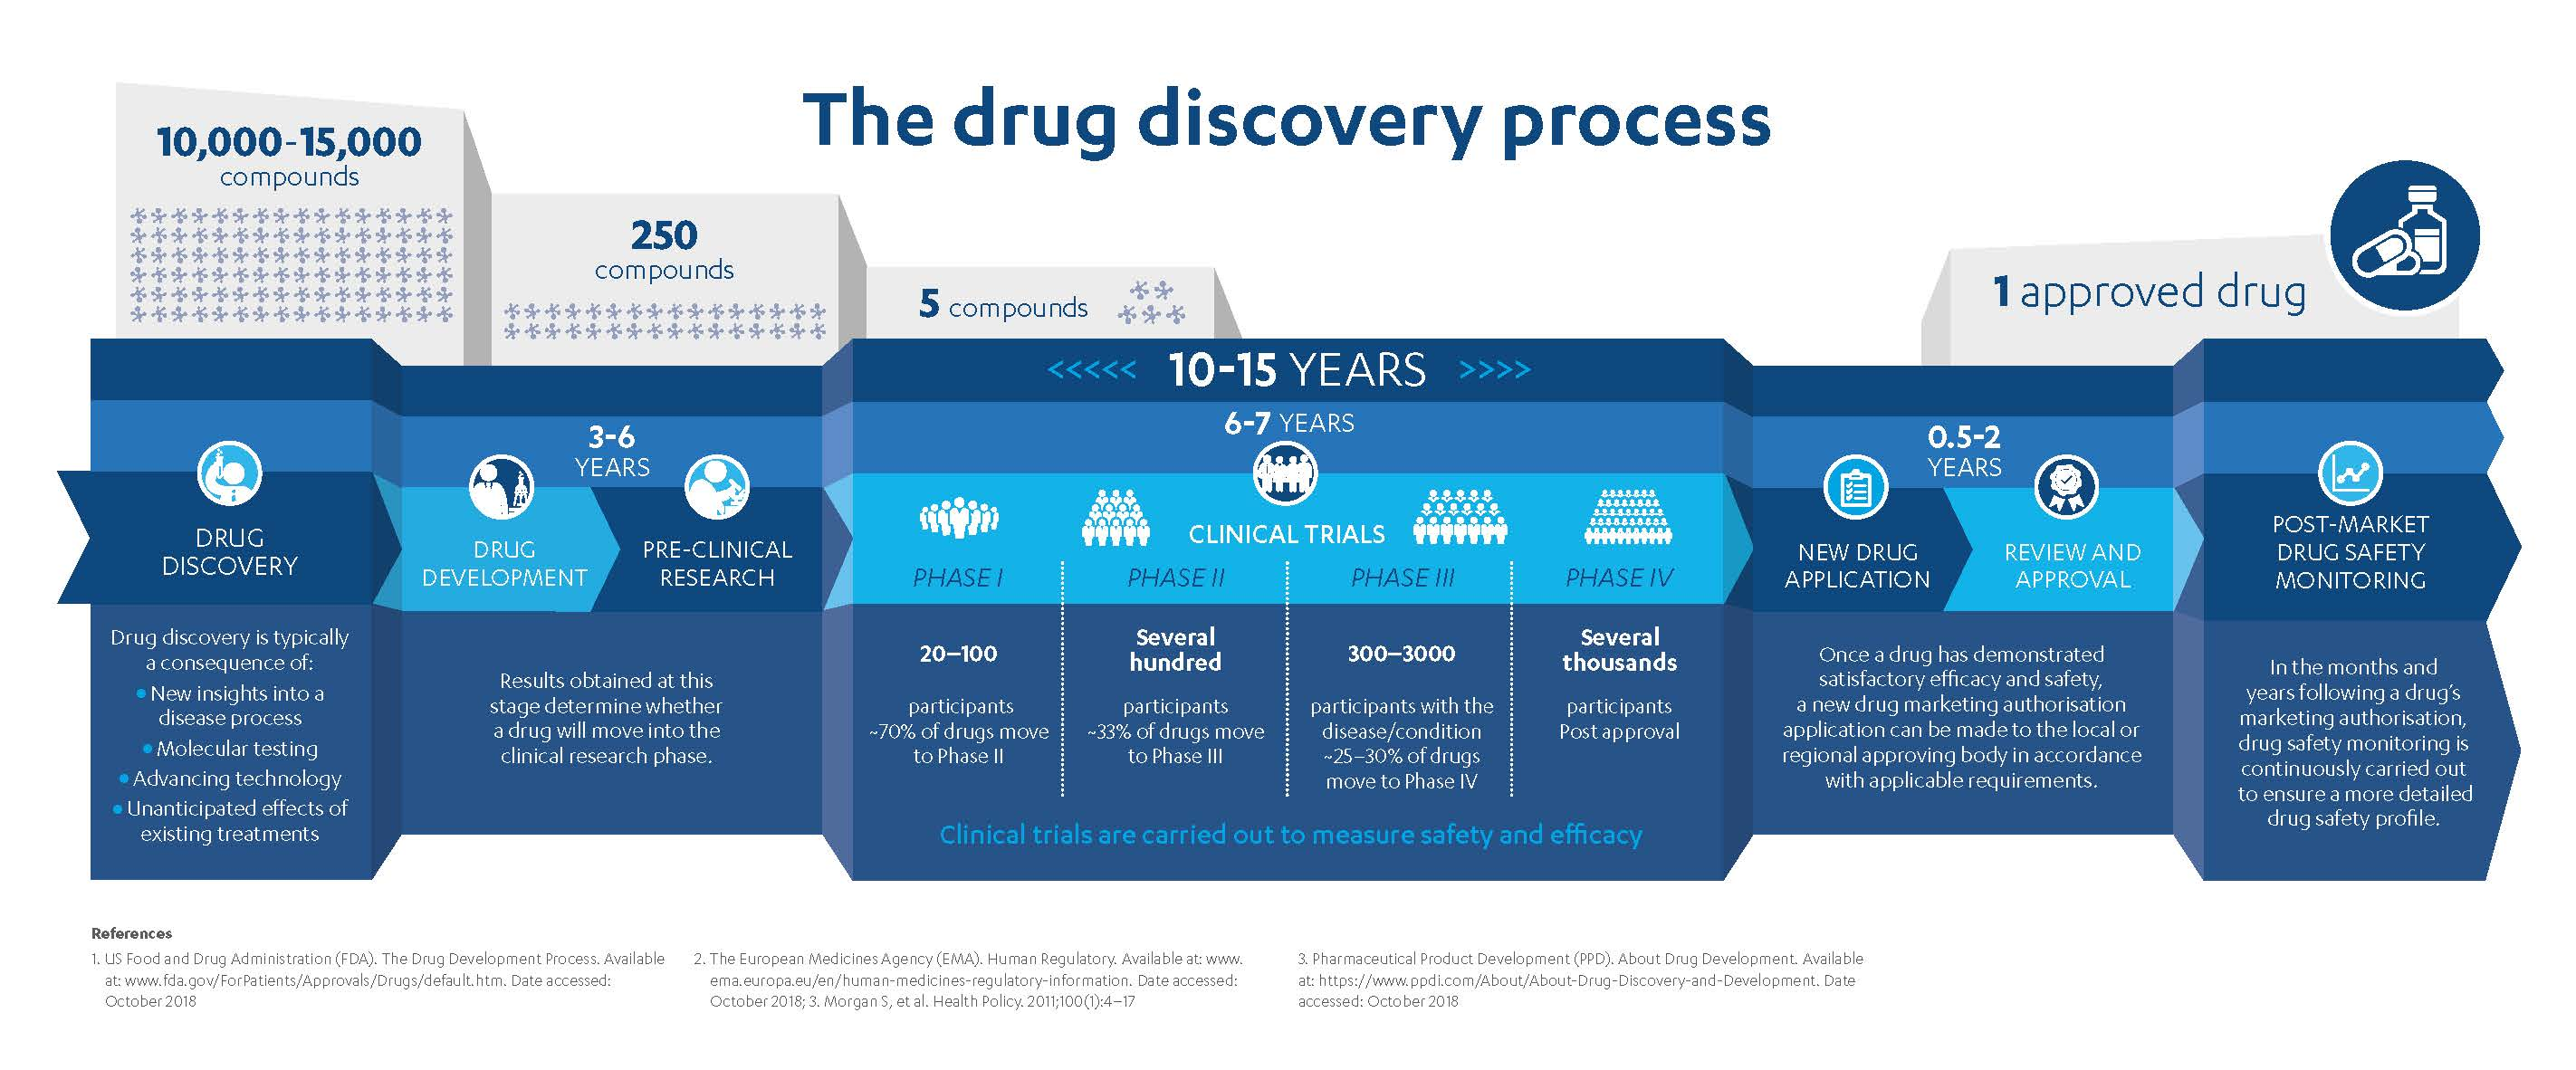
\includegraphics[width=1.3\textwidth,center]{drug-discovery}
  \caption{The traditional drug discovery pipeline \citep{janssen2019}}
  \label{fig:drug-discovery}
\end{figure}

% During the first phase, the properties tested \textit{in vitro} fa

% ADME, Tox, biological activity



\subsection{Computational drug discovery}
\label{sec:computational}

Imagine you could completely predict the properties of a compound as well as its effects on the human body \textit{in silico} (that is, computationally). Such capabilities would enable us to bypass the time-consuming process of quasi-randomly testing molecules during the pre-clinical phase. Instead, we would first use computational bio-chemistry to pre-select a handful of compounds, whose \textit{in vitro} and \textit{in vivo} testing would become a mere formality. Drug discovery would be revolutionised by such a technical leap.

Artificial intelligence holds the promise of enabling not only fast and accurate pre-screening, but also direct compound optimisation for a set of properties. With such a technology at disposal, new insights into the operation of a disease would be translated into a set of active molecules ready for human trials in a matter of days, leading to a new treatment shortly thereafter.

Computational drug discovery can be summarised into three distinct but coupled problems:
\begin{enumerate}
  \item \textit{Scoring}. ``Scoring'' a molecule, or estimating its properties, is the first building block of an artificial intelligence that can help discover new drugs. Computational biochemists talk of \textit{quantitative structure–activity relationship} (QSAR) modelling. The properties regularly tested are known as ADME/Tox for ``absorption, distribution, metabolism, excretion'' and toxicity.

  \item \textit{Generation}. There are an estimated $10^{60}$ possible small molecules \citep{chemicalspace}, while the largest molecular databases hold at most a hundred millions of them. Until now, the industry has been relying on candidate compounds with poor diversity relative to the unfathomable size of the unexplored chemical space.

  \item \textit{Optimisation}. Combining a good generation strategy to efficiently explore the space of small molecules and an accurate scoring function, we may one day be able to optimise for compounds directly: given a set of desirable properties, the algorithm would propose candidates that are designed to perform best.
\end{enumerate}

Of course, scoring is the main piece of the puzzle. We can handle a poor generative model, by relying on empirical (and often random) methods used in the field until now. Although the candidate compounds will be the same, a good scoring model means that candidates are first tested and screened \textit{in silico}, before a significantly lower share moves on to lengthier and costlier \textit{in vitro} and \textit{in vivo} testing. Conversely, we cannot optimise if the scoring model itself is unreliable.

At InVivo AI, we primarily focus on scoring molecules, by developing algorithms able to propose chemical compounds that have a high probability of scoring well on every desirable properties, thus limiting tremendously the amount of time and money needed on the first pre-clinical phase. At the same time, we actively develop generative and optimisation models, such that they may use the most recent and state-of-the-art methods for scoring as they come out.

Last, note that an algorithm that scores well necessarily uncovered patterns in the molecular structures. Said patterns can be analysed by chemists, leading to new insights and helping the scientific community in the exploration of high-potential avenues of research.


\subsection{The challenges ahead of computational drug discovery}

Computational drug discovery is a formidable endeavour and its success can be broken down to smaller challenges. To wit, computational biochemists need to address many sub-problems :
\begin{enumerate}
  \item \textit{Representation}. Learning from data in a well-structured environment, such as inferring tree height from tunk circonference (a well-known and almost toyish regression problem), is considerably easier than learning from heterogeneous data. Hence, the very first question computer scientists and biochemists need to answer deals with the representation of molecules.

  \item \textit{Extrapolation}. As we have established, the molecular space is vast. By focusing on an infinitesimal portion, we effectively limit ourselves to compounds that have a very low probability of being the optimal treatment for a given disease. However, scoring significantly different compounds implies that the algorithm is able to extrapolate beyond the molecular subspace it was trained on.

  \item \textit{Data efficiency}. One of the main obstacles to the advent of artificial intelligence in the field of drug discovery in the small amount of data. Hence, we need to devise methods and training strategies that can learn efficiently from very few datapoints.

  \item \textit{Calibration}. For a scoring algorithm to be useable in critical applications, it should be able to assess its level of confidence on its predictions.
\end{enumerate}



\subsubsection{Representation}

The very first challenge that computational bio-chemists need to address before artificial intelligence can help drug discovery is the representation of the molecules. Indeed, there are many ways of describing a chemical compound, but the canonical representations are not readily applicable to machine-learning algorithms, which work with tensor data.

We can formulate a few desiderata regarding a suitable molecular representation, which needs to be :
\begin{itemize}
  \item Informative. Artificial intelligence has become extremely effective at recognising patterns within the data it is presented with. However, it goes without saying that the prediction can only be as good as the information conveyed by the representation.

  For instance, molecular formulae only convey the number of atoms from each element present in the molecule, thus glossing over important configuration details that can dictate whether the molecule is a cure or a poison.
   % Hence, they are not informative enough for our purposes.

  \item Structured. Machine learning algorithms work primarily with tensor data. Over the years, computer scientists have develop methods to treat images, textual data, and even graphs.

  Depending on the representation we choose, some of these methods can be applied directly.
\end{itemize}

% \begin{figure}[ht]
%   % \makebox[\textwidth][c]{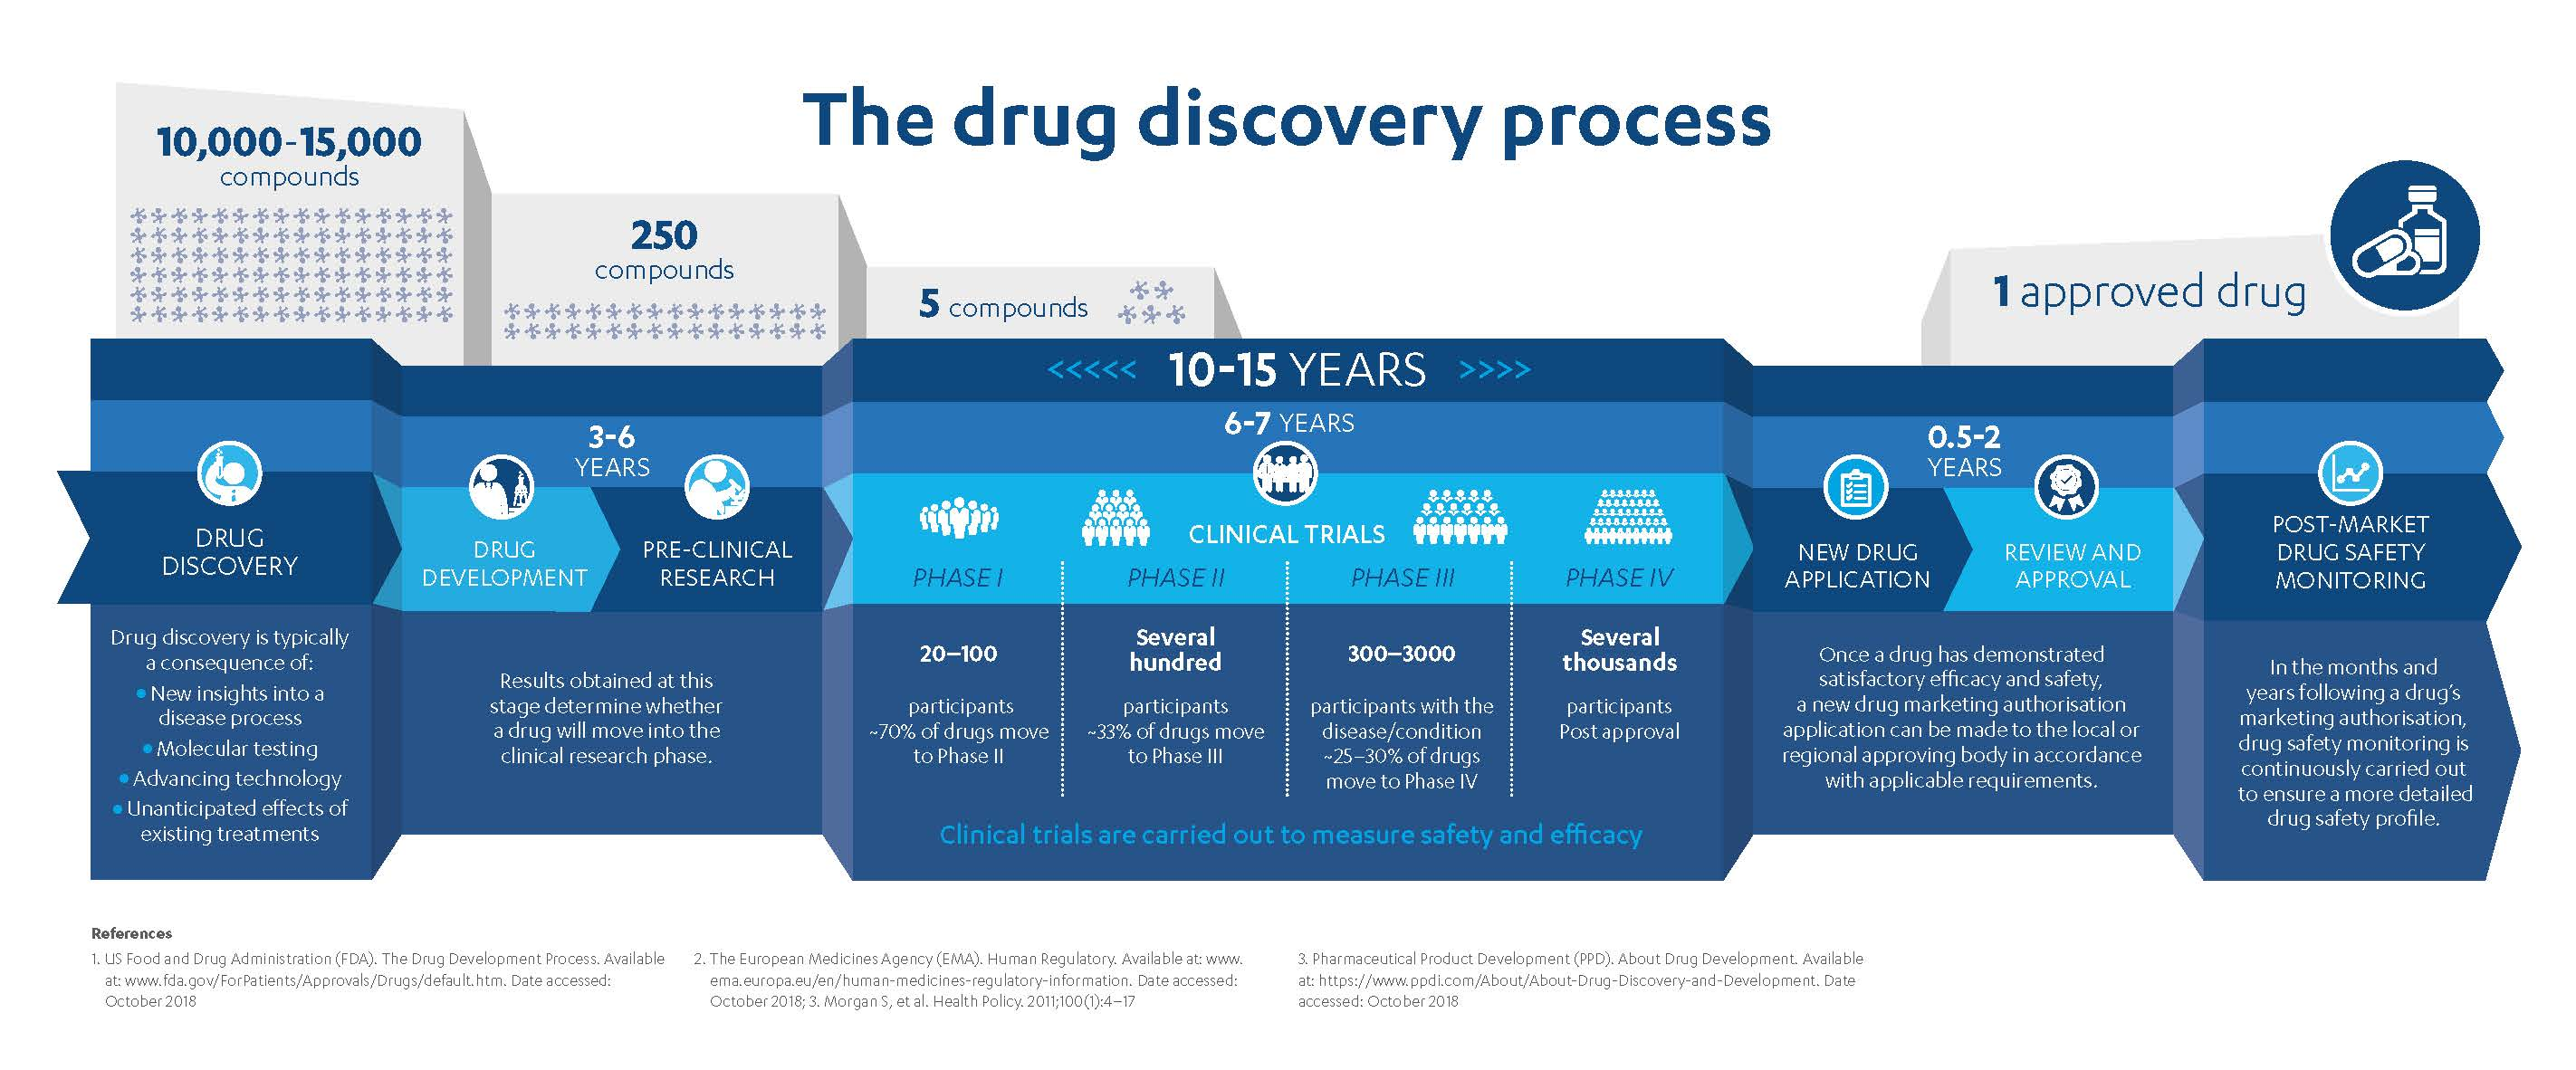
\includegraphics[width=1.3\textwidth]{drug-discovery}}
%   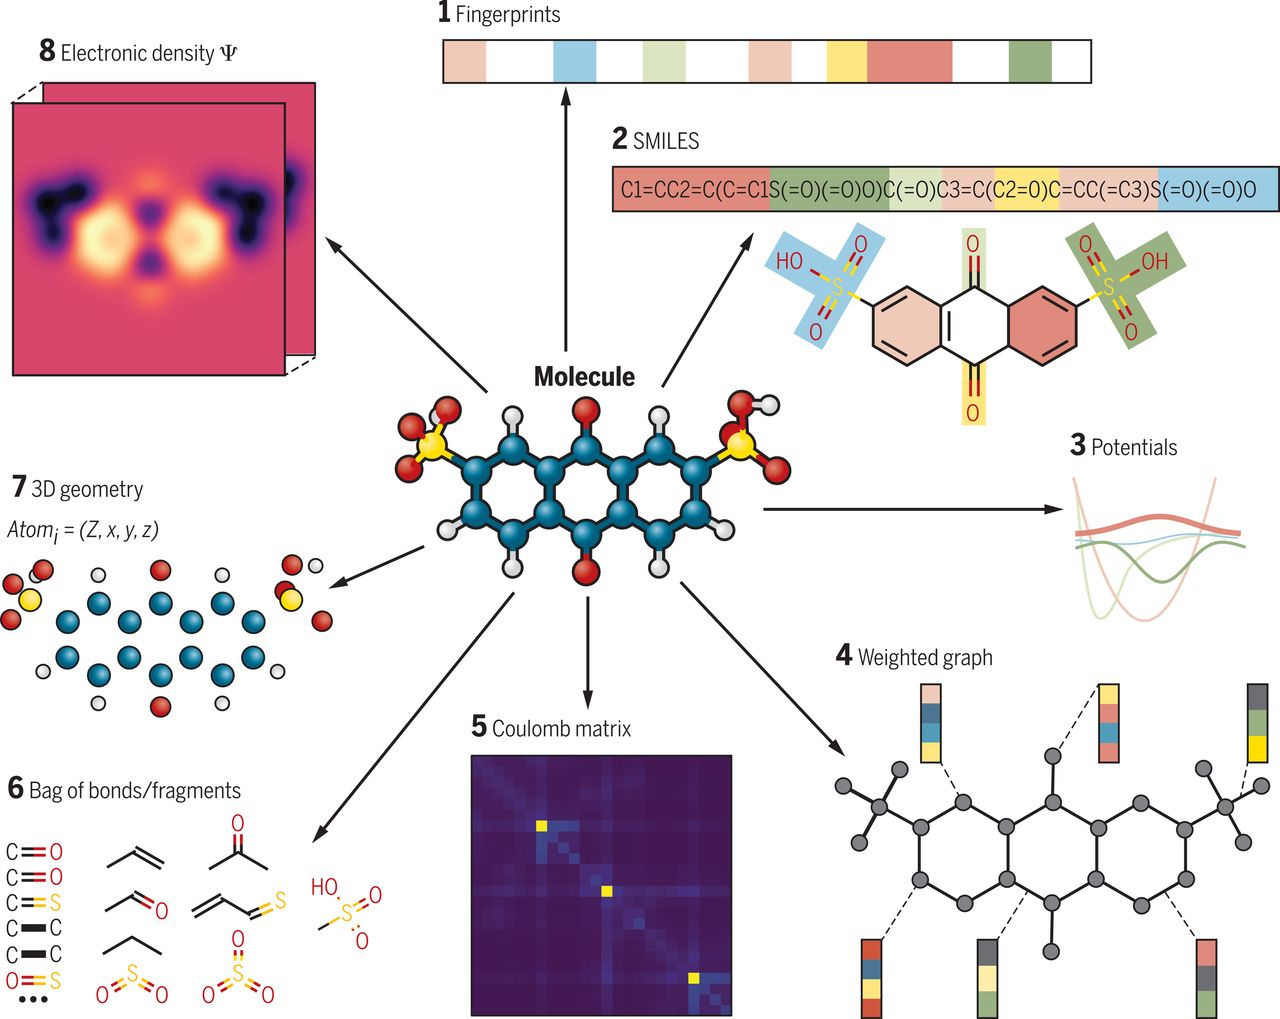
\includegraphics[width=1\textwidth,center]{representation}
%   \caption{Different ways of representing a molecule \citep{sanchez-moleculardesign2018}}
%   \label{fig:representation}
% \end{figure}
%
% \Fig{representation} presents eight possible representations for a given molecule. Although I will describe them in more details later in the report (namely in the state-of-the-art section), let us gloss over some of them.
%
% \begin{itemize}
%   \item The SMILES (2) description is a textual representation that uniquely characterise a given molecule. The community can use well-established methods borrowed from natural language processing to extract its information.
%   \item The 3D geometry (7) is able to account for the full conformation of the molecule, and thus conveys important information. However, it remains a poorly structured representation not usable as is by a machine-learning algorithm.
%   \item Fingerprints (1) are the most readily usable representation, since it describes a molecule by a binary vector, that is, a vector of ones and zeros that encode the presence or absence of a set of substructures.
% \end{itemize}

Astonishingly, a team of researchers obtained near-state-of-the-art results by using the two-dimensional representation of molecules, fed as images to an Inception-like convolutional neural network \citep{goh2017chemception}. However, I for one do not expect this avenue to be the future of drug discovery. Molecules are well-structured objects, and thus naturally call for inductive biases to be included in the way we represent and treat them. Using images breaks that structure, and needs the network bore the burden of understanding chemistry from bonds described by pixels, a remarkably unnatural representation indeed.


\subsubsection{Compositionality and extrapolation}

Given the immensity of the molecular space, it quickly becomes paramount to be able to extrapolate, at least to some extent, the insights gathered on the training data to unseen regions of the molecular space.

However, the above statement is problematic. As of today, machine-learning algorithms are essentially function approximators that are very effective at \textit{interpolating} between datapoints, provided there come in sufficient numbers. On the other hand, extrapolation is not only elusive but also impossible without formulating some heavy assumptions on the structure of the problem.

Consider \fig{extrapolation}, that represents four univariable functions that coincide perfectly on some region of the reals. Imagine now that we train an algorithm on the shared portion of the $x$ axis: how could it decide which function best describes the training data once we go beyond their scope ?

\begin{figure}[ht]
  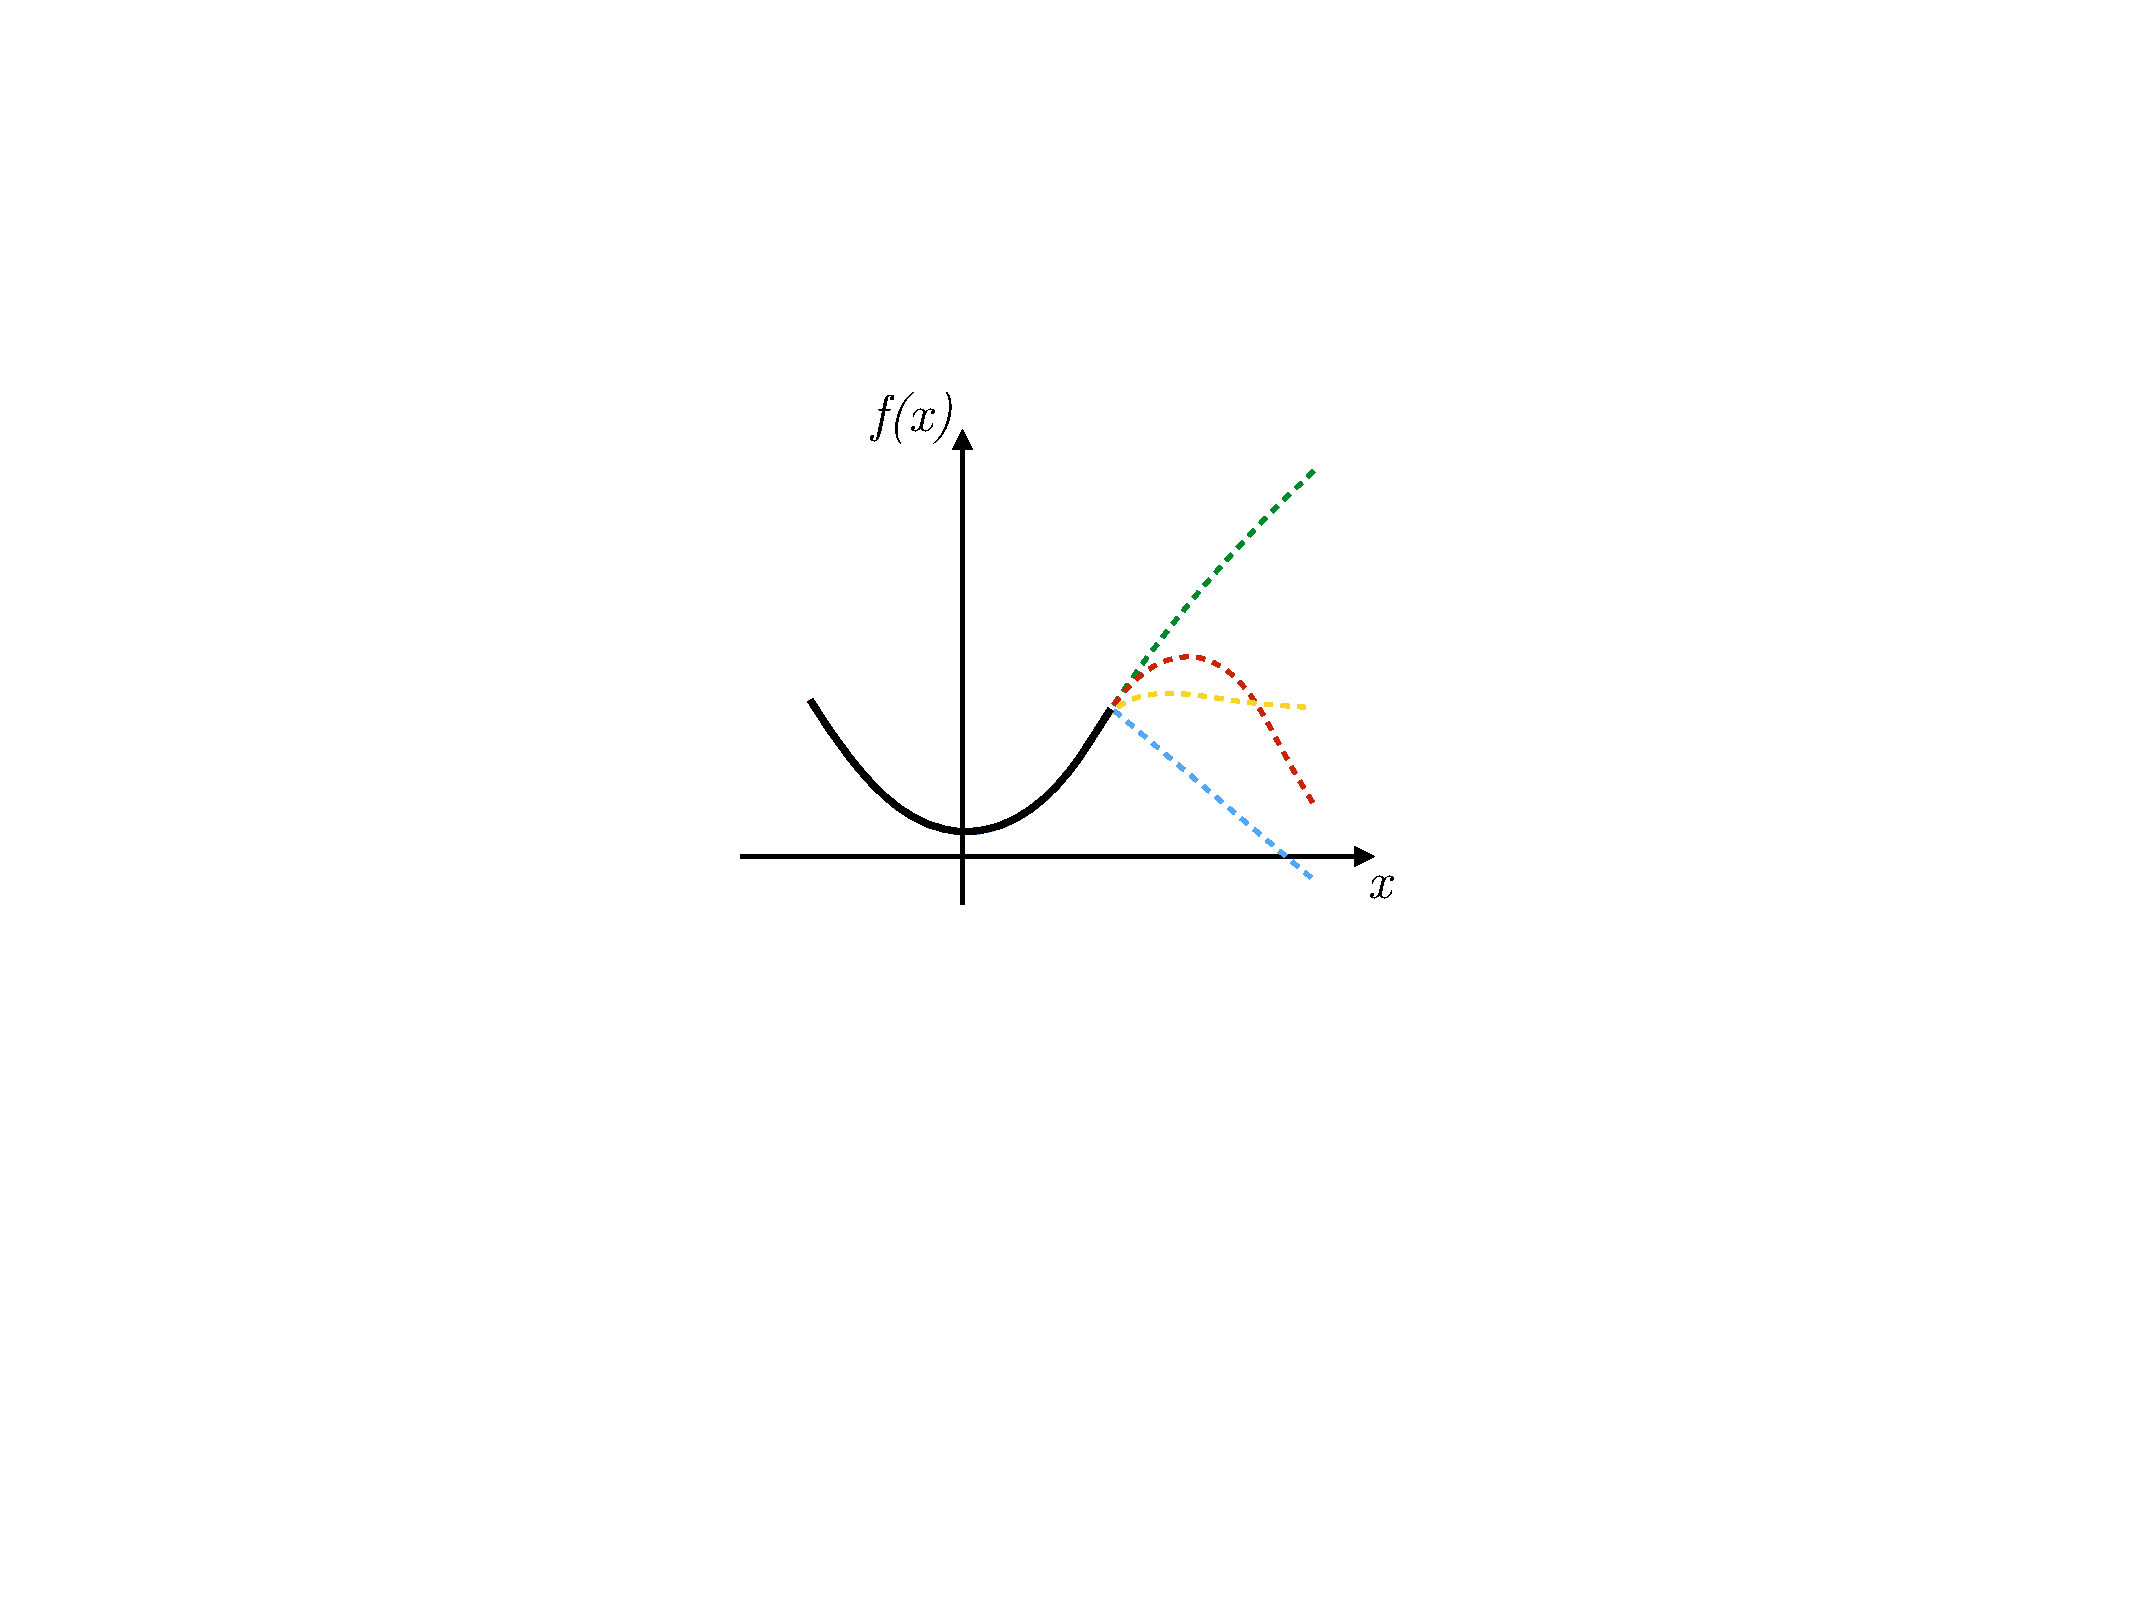
\includegraphics[width=.4\textwidth,center]{extrapolation}
  \caption{Which one do we choose ?\\Four functions that coincide...}
  \label{fig:extrapolation}
\end{figure}

In the case of drug discovery and more specifically molecular scoring, the underlying hypothesis that lets us hope to one day extrapolate beyond the scope of the training data is the \textit{compositionality} assumption. In a compositional problem we can derive some law that governs, at least to some extent, the observed phenomenon. Hooke was able to formulate his law linking the force needed to extend a spring to the elongation of the latter precisely because that problem is indeed compositional.

% \begin{wrapfigure}{l}[2.0cm]{0.45\textwidth}
%   \centering
%   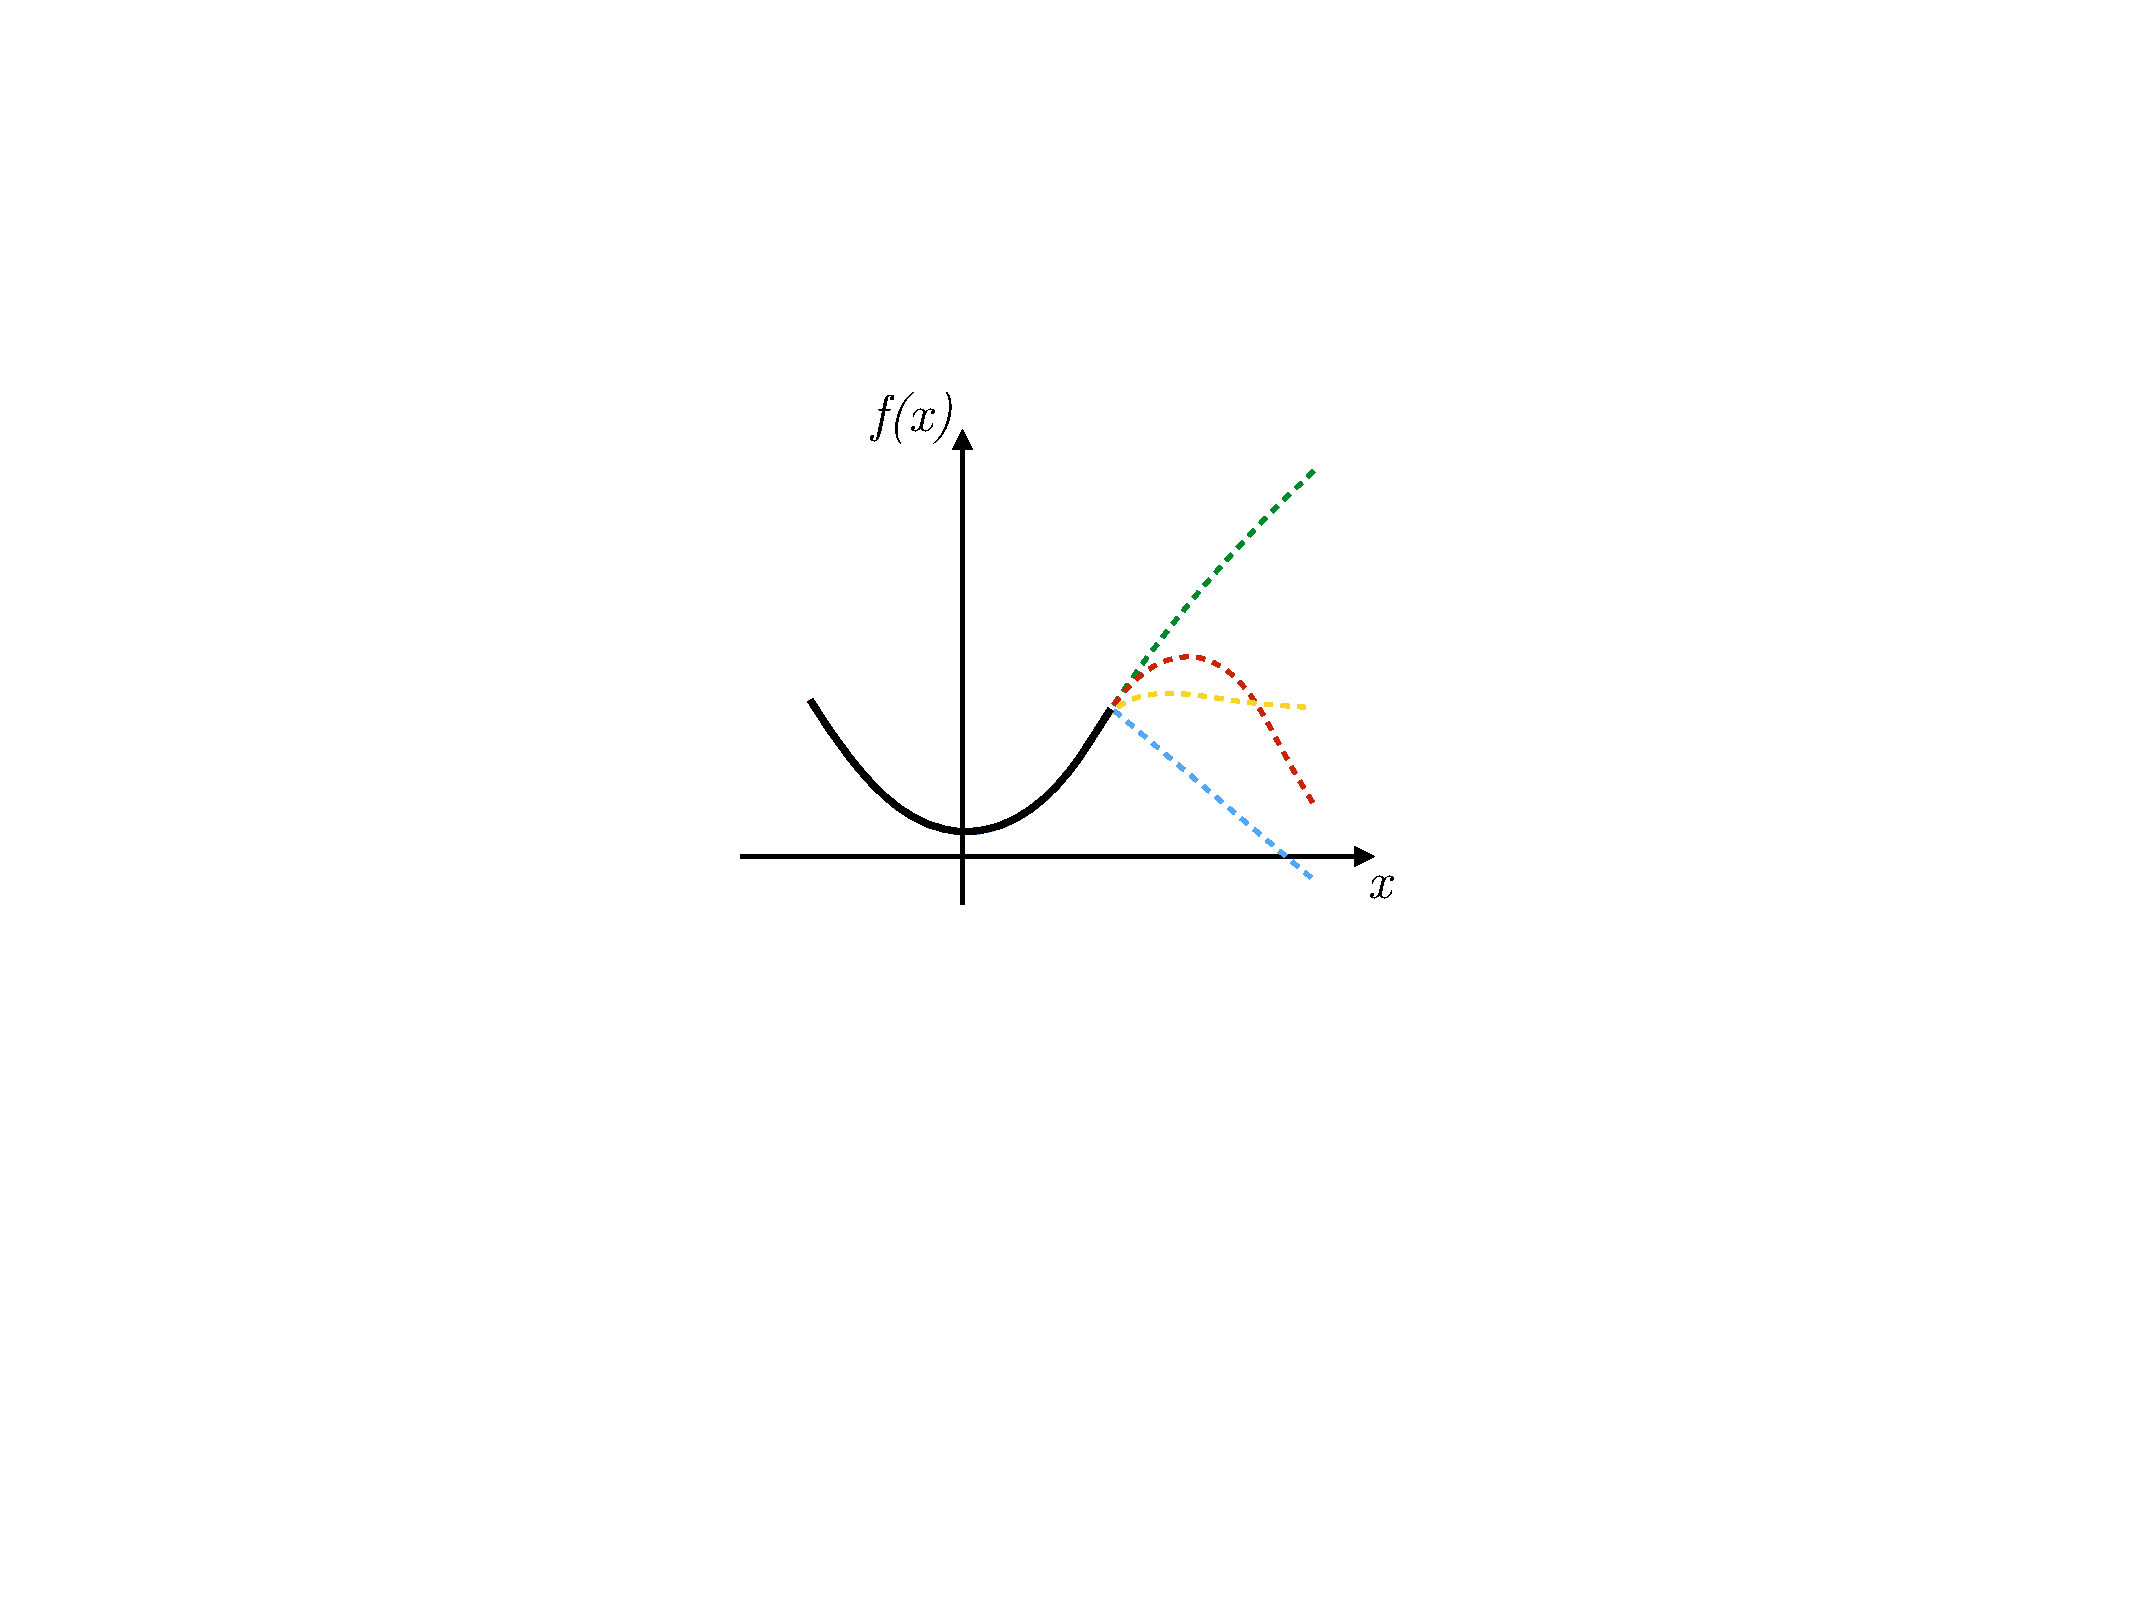
\includegraphics[width=.9\linewidth,center]{extrapolation}
%   \caption{Which one do we choose ?\\Four functions that coincide...}
%   \label{fig:extrapolation}
% \end{wrapfigure}

If you can retrieve the compositional structure of a problem, provided it exists, then you get two precious assets. First, the amount of data needed to train your model is substantially reduced: in the case of Hooke's law, you only need a single measurement to estimate the stiffness of the spring. Second, the compositional nature of the problem means that you may apply it far from the training examples.

Hence, we posit that much of a compound's activity is driven by the interactions between its chemical substructures, along with some fringe region-specific adjustments. That is to say, we do not discart region-specific knowledge as non-informative. Rather, we hypothesise the bulk of a compound's property can be inferred by looking at features that are compositional, and thus apply in a broader region of the molecular space.

At this point, you might get anxious that the assumption may not hold, and computational drug discovery be doomed. Let me share some reassuring thoughts.
\begin{itemize}
  \item First, we know that compositionality exists in the realm of molecular properties. Indeed, it is the only reason chemistry itself, as a discipline, exits.

  \item Second, computational drug discovery itself does not rely on extrapolation. Should the compositionality assumption break, we would be forced to stick to the limited scope of the training data. But keep in mind that it still represents plenty of samples to go through, and traditional drug discovery has thriven without extrapolation since its beginnings.
\end{itemize}



\subsubsection{A fundamentally low-data problem}
\label{sec:low-data}

When computer scientists design a machine-learning algorithm, they merely build an architecture. The whole idea of artificial intelligence is to \textit{train} the machine rather than set its parameters by hand. And in order to train the algorithm, computer scientists need labelled data.

Depending on the complexity of the problem we would like to solve, our algorithm might need formidable amounts of data: in fact, there is a tradeoff between the expressivity of a network and the data efficiency of the training phase.

For instance, a simplest linear regression model will need very few points to be trained, but will not be capable of capturing complex patterns. At the far end of the spectrum, you will find mamoth-sized networks such as BERT \citep{devlin2018bert}, a state-of-the-art language representation model with 304 million parameters and trained on a 3,300 million word corpus\footnote{Unlike molecular scoring, language representation is an inherently self-supervised task: any sentence or paragraph written in the language you are training on is a valid example, which helps gather massive amounts of data.}.

In the case of drug discovery and molecular scoring, we can safely assume that the relationship between the structure of a molecule and its properties requires a high expressivity to model the intricacies of molecular activities. Consequently, computational drug discovery is an inherently data-hungry process.

In the drug discovery context, labelled data come from past trial campaings wherein a myriad of studies are performed on the candidate compounds to have a sense of their activity, solubility, toxicity, and so on. In such studies, called biological assays or bioassays, only a handful of molecules are tested at a time. What is more, each bioassay reports the activity of these compounds relating to a very specific property. For instance, one such study might report the antibacterial effect of a few molecules on a specific strain of bacteria.

In other words, each bioassay pertains to a different machine-learning problem, with very little overlap. Moreover, for each of these problems, saying that data is scarce would be an understatement –and remember that modeling a bioassay is a most complex endeavour.

To give more substance, let us consider two bioassay collections that we at InVivo AI introduced in 2019. Compiling datasets coming from the public domain (\href{www.bindingdb.org}{BindingDB} and \href{https://pubchem.ncbi.nlm.nih.gov/}{PubChem} ), we proposed the community use the \hyperref[app:collections-binding]{\texttt{Binding}} and \hyperref[app:collections-antibacterial]{\texttt{Antibacterial}} collections, that are \href{https://github.com/invivoai/molecular-datasets}{available here}\footnote{The full URL for the paper version: \href{https://github.com/invivoai/molecular-datasets}{\texttt{https://github.com/invivoai/molecular-datasets}}}.
% In the \texttt{Binding} collection, each bioassay reports the binding affinity of a set of molecules to a single protein while in \texttt{Antibacterial} they describe the antibacterial effect of the tested molecules on a particular strain of bacterium.
See \append{collections-real} for a thourough description of the collections.

\begin{figure}[ht]
  \makebox[\linewidth][c]{
    \begin{subfigure}[t]{.38\textwidth}
      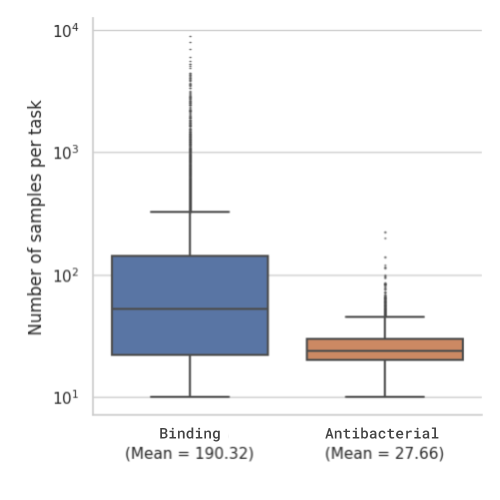
\includegraphics[width=1\textwidth,center]{datasets/samples}
      \caption{Number of samples}
      \label{fig:dataset-description-samples}
    \end{subfigure}
    \hfill
    \begin{subfigure}[t]{.49\textwidth}
      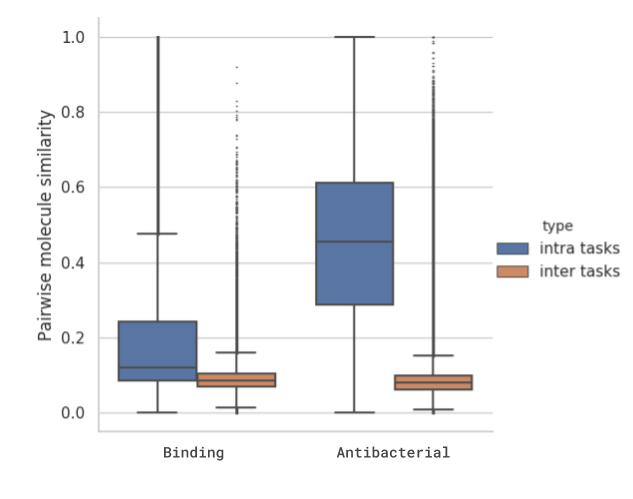
\includegraphics[width=1\textwidth,center]{datasets/similarity}
      \caption{Similarity between molecules}
      \label{fig:dataset-description-similarity}
    \end{subfigure}
    \hfill
    \begin{subfigure}[t]{.38\textwidth}
      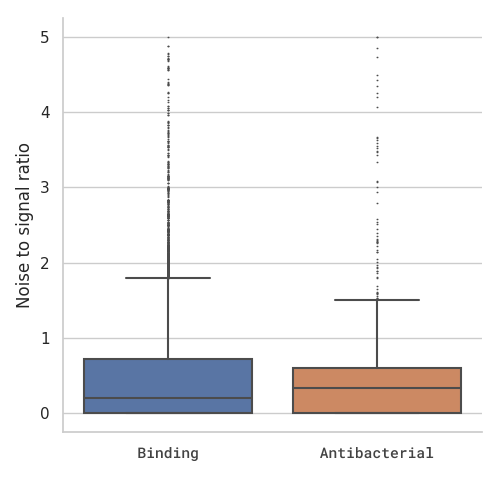
\includegraphics[width=1\textwidth,center]{datasets/snr}
      \caption{Signal to noise ratio}
      \label{fig:dataset-description-snr}
    \end{subfigure}
  }
  \caption{A few statistics for the \texttt{Binding} and \texttt{Antibacterial} collections}
  \label{fig:dataset-description}
\end{figure}

The two collections epitomise the scarcity of data in the discipline. \Fig{dataset-description-samples} illustrates that issue eloquently, by reporting the number of compounds that are tested for  \texttt{Binding} and \texttt{Antibacterial}: the average number of molecules tested in a single bioassay is as low as 190 for the \texttt{Binding} collection and 28 for the \texttt{Antibacterial} collection ! Remember, Inception \citep{inception} was trained on 1.2 million images... Although computational drug discovery necessitates huge numbers of examples, it remains a fundamentally low-data problem. We need to reconcile this apparent contradiction.

But scarcity is not the only issue. Looking at \fig{dataset-description-snr}, we quickly realise that data is not only limited but also incredibly noisy. Indeed, the noise-to-signal ratio (computed on the measurements that were done twice or more) is extremely high, an additional challenge for training machine-learning algorithms.

% Although drug discovery necessitates huge numbers of examples, it remains a fundamentally low-data problem. We need to reconcile this apparent contradiction.

Moreover, a concern raised in the previous section about extrapolation is already dicernable in the two collections. To wit, \fig{dataset-description-similarity} shows that molecules are much more similar\footnote{Here similarity is computed for molecule pairs using Tanimoto's similarity with ECFP4 on 2048 bits (see \sect{fingerprints}).} within a bioassay than accross them, which suggests that the results will be hard to generalise even to known molecules without some kind of extrapolation strategy.

The diagnosis is unequivocal: drug discovery is an inherently low-data problem. Data is not limited \textit{per se}: rather, data related to each individual property is painfully scarce. Now, how do we go about working towards a solution? Two directions are before us:
\begin{enumerate}
  \item We may work towards automating \textit{in vitro} testing, to be able to collect data with a more systematic approach. The amount of data would increase dramatically, along with its quality.

  \item We can also develop novel methods that extract information from seemingly unrelated studies or bioassays. The underlying assumption is that the different molecular properties are dictated by the structure of the compounds, which can be learned across bioassays.
\end{enumerate}

These two approaches are not mutually exclusive. Surely, having better machine-learning methods would help the first approach, much like cleaner and more abundant data will certainly help the second avenue. However, while the former necessitates huge investments to develop and produce automated test machines, the latter can benefit from the data that is already available --be it in the public domain or not. At InVivo AI, we have chosen to focus on the second approach.


\subsubsection{Calibration}

Imagine you are a cartographer, looking to construct a map of an unknown world. You have explorers at you disposal, that you can pay to explore a specific part of the land and thus improve the precision of the map. In order to maximize the information obtained about the world, you should send your explorers to regions for which you have minimal information, rather than places for which you already have a somewhat precise idea.
% This is precisely what active learning is all about.

However, to be able to do that, a cartographer needs to assess its confidence in the precision of the current map. Your explorers are flawed –aren't we all?–, and might give you less than reliable insights on the New World.

In the context of drug discovery, we are building a map of the molecular space. We do not send explorers to the far corners of the world: rather, we ask researchers to perform experiments in the form of bioassays. But those may be noisy, and are certainly costly.

Hence, another desirable property for our algorithms is for them to be aware of their shortcomings. More formally, an algorithm capable of correctly assessing the confidence interval around its predictions (what is called calibration) can come extremely handy in the setting of biochemistry. Indeed, the limited amount of data and the high acquisition cost mean that being able to pinpoint the compounds that will give the most information when tested has enormous advantages.

With a well-calibrated algorithm, you can guide the \textit{in vitro} testing of new compounds in such a way that maximizes the information you get about the world when you generate new labels. This is called \textit{active learning}: you have a set of labelled examples and a collection of samples for which you can get new labels at a cost, and the goal is to select for which of those samples you will pay to get labels.



\clearpage
\section{Traditional machine-learning for drug discovery}

In the previous section, I set out to discuss the challenges that computational drug discovery faces to reach its enormous potential as a revolutionising tool for biochemistry.

The machine-learning community has already made huge progress in tackling these challenges, and this section is dedicated to presenting some of the ideas that have been proposed. It will be the opportunity for me to give a more formal presentation of machine-learning applied to drug discovery, which will surely please the more mathematics-enthused reader.

I will focus on two aspects of drug discovery: representation and scoring. Bear in mind that this section is by no means an comprehensive enumeration of the state-of-the-art methods used today in the field. Rather, it is meant as a collection of examples whose goal is to better illustrate the stakes of using artificial intelligence in drug discovery, and how fundamental research in machine-learning has provided ways to address some of those challenges.


\subsection{Representation}
\label{sec:representation}

Before we can effectively train an algorithm to recognise the extremely compex patterns that govern molecular activity, we need a representation method that satisfies two main \textit{desiderata}:
\begin{enumerate}
  \item The representation method must be adapted to a machine-learning algorithm, that is to say either presented as a tensor or as an object that we know how to transform into a tensor.
  \item The representation method needs to include as much information as possible. Otherwise, the algorithm will not be able to perform the downstream task.
\end{enumerate}

% \Fig{representation} presents eight possible representations for a given molecule. Let us gloss over some of them.

\begin{figure}[ht]
  % \makebox[\textwidth][c]{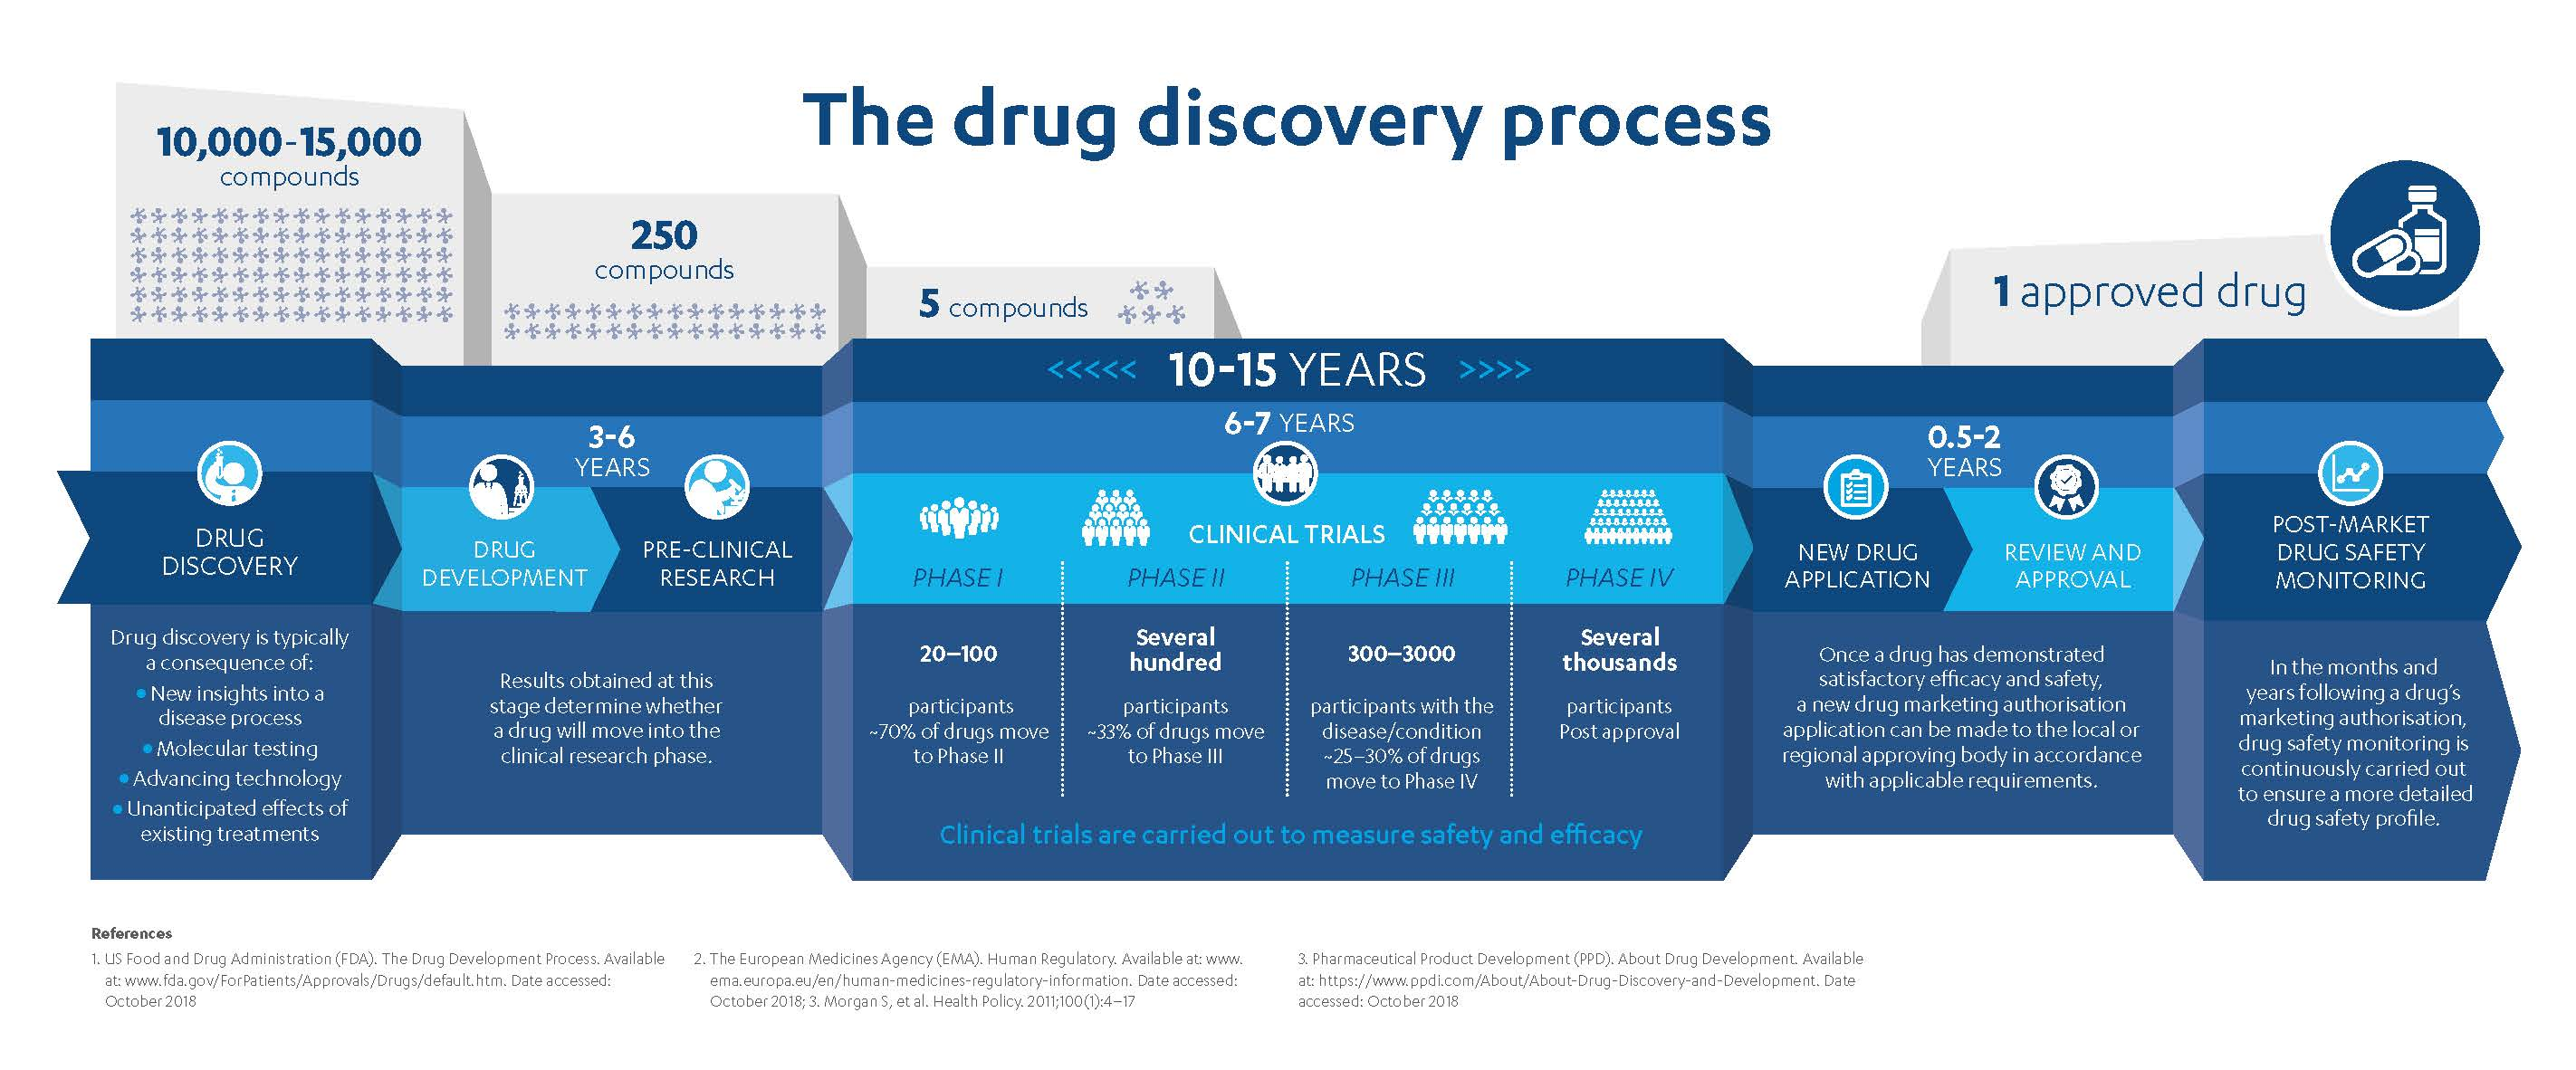
\includegraphics[width=1.3\textwidth]{drug-discovery}}
  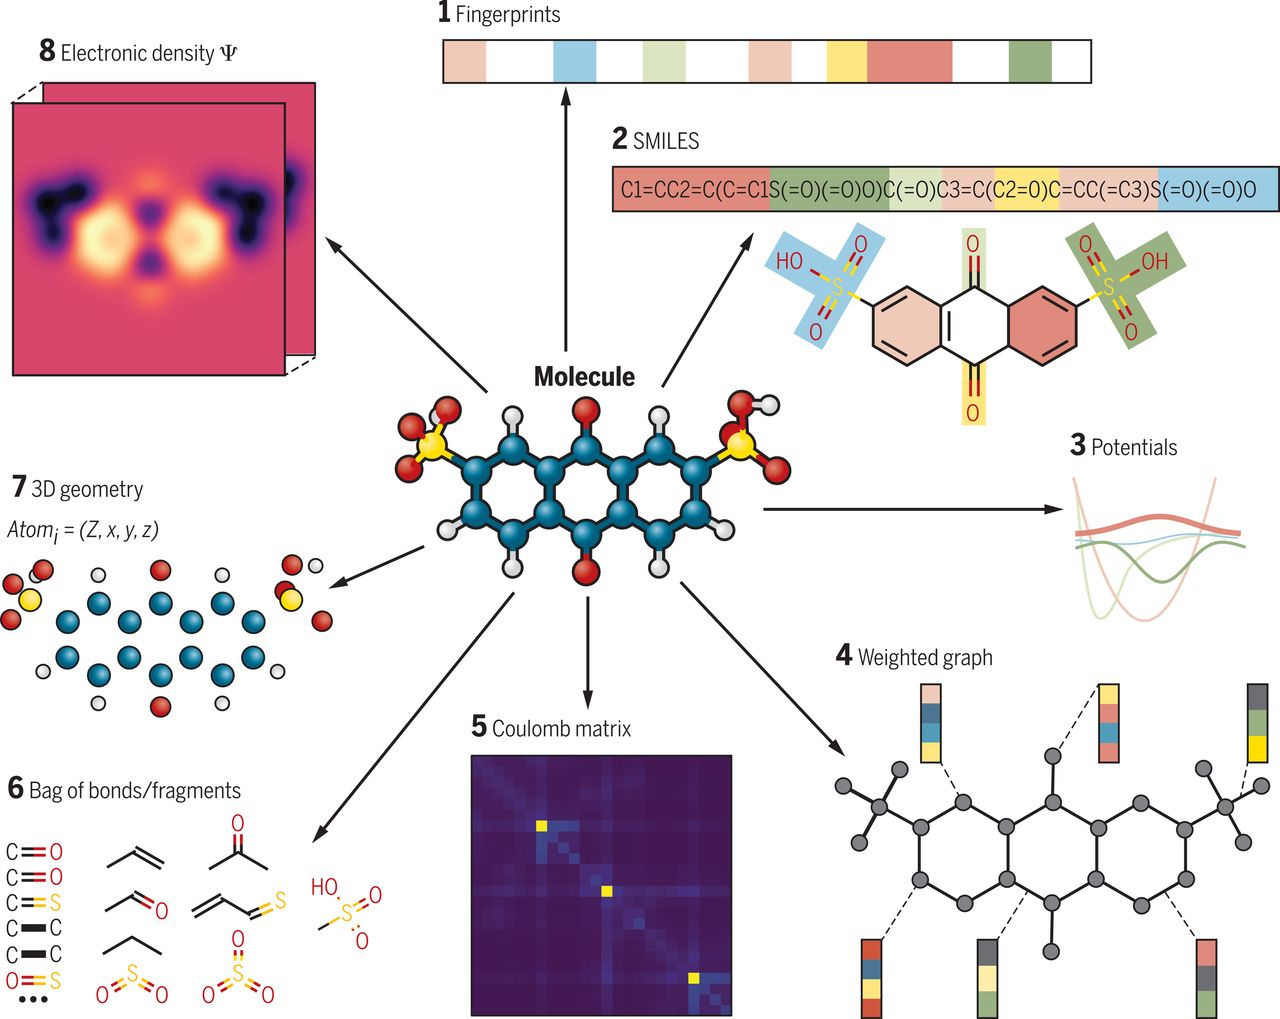
\includegraphics[width=1.05\textwidth,center]{representation}
  \caption{Different ways of representing a molecule \citep{sanchez-moleculardesign2018}}
  \label{fig:representation}
\end{figure}

\Fig{representation} presents eight ways to represent a given molecule that can be used in machine-learning. Let us gloss over some of them:
\begin{itemize}
  \item Fingerprints (1) are the most readily usable representation, since they describe a molecule by a binary vector, that is, a vector of ones and zeros that encode the presence or absence of a set of substructures.
  \item The SMILES description (2) is a textual representation that uniquely characterises a given molecule. The community can use well-established methods borrowed from natural language processing to extract its information.
  \item The 3D geometry (7) is able to account for the full conformation of the molecule, and thus conveys important additional information. However, it remains a poorly structured representation not usable as is by a machine-learning algorithm.
\end{itemize}


% First, the representation method must be adapted to a machine-learning algorithm, that is to say either presented as a tensor or as an object that we know how to transform into a tensor. Second, the representation method needs to include as much information as possible. Otherwise, the algorithm might not be able to perform the downstream task.

At InVivo AI, we primarily use SMILES and fingerprint, since they are easy to produce and achieve good performance. In the following, I will focus on the two and them in more depth.


\subsubsection{The SMILES representation}

The \textit{simplified molecular-input line-entry system}, or SMILES (not a plural), provides a convenient, human-readable and normalised way to represent molecules. It was proposed by \citet{smiles}.

The principle is straightforward: the system provides a way to describe the molecular structure of a compound by defining the rules that govern how the molecular graph should be traversed in order to obtain unambiguous string representations. \Fig{smiles} proposes an example of that procedure: the algorithm breaks the cycles, defines a main chain and describes the branches according to the syntaxic and grammatical rules of the SMILES notation system.

\begin{figure}[ht]
  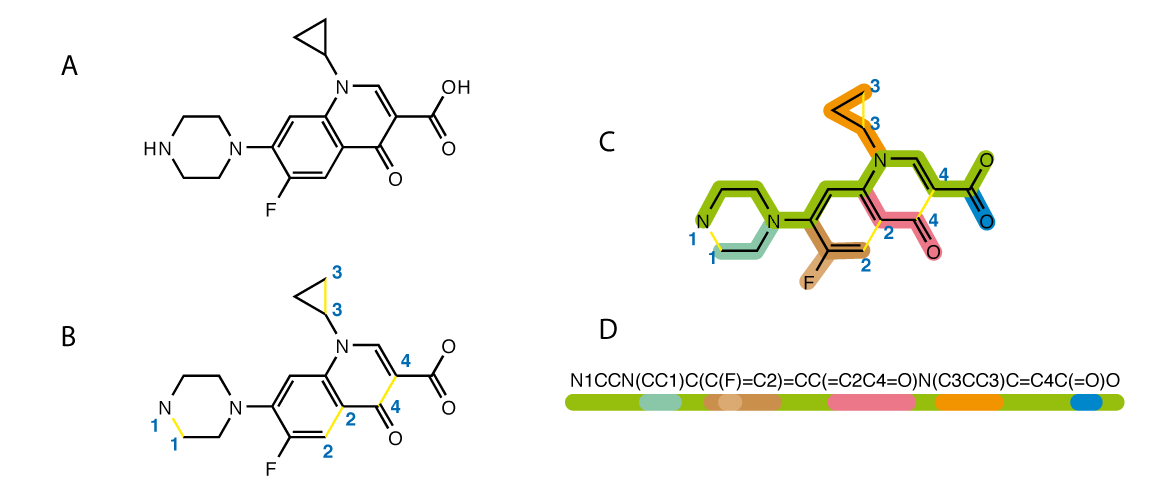
\includegraphics[width=.7\textwidth,center]{representation/SMILES}
  \caption{Construction of the SMILES notation for Ciprofloxacin; the algorithm \\breaks the cycles, defines a main chain and describes the branches \citep{wiki:smiles}}
  \label{fig:smiles}
\end{figure}

Hence, SMILES yields a string notation that fully describes the 2D configuration of the molecule. As such, it is a particularly rich representation, since it can uniquely represent any molecule.

Moreover, although it cannot be used directly in a machine-learning setting, it may as well be: tremendous progress made in the field of natural language processing (NLP) have led to extremely effective algorithms (namely ``recurrent neural networks'', or RNNs) to work with textual data governed by syntaxic and grammatical rules.

Hence SMILES is not a complete representation in a machine-learning sense: it is merely a convenient intermediary notation that relies on an auxiliary network whose role is to provide a meaningful tensor representation. One question remains: how do you train that auxiliary network? You have two main possibilities, which are not exclusive:
\begin{enumerate}
  \item You can train the entire network in an end-to-end fashion, meaning that the representation is learned to minimise the error on the task you are training on.

  \item Alternatively, you might want to pre-train the ``auxiliary network'', using unsupervised learning.
\end{enumerate}

The first solution adds a potentially large number of parameters to the trained model, and thus may necessitate vast amounts of data. As such it might not be the best choice in our context, even though it would learn features more specific to the problem at hand.

The second solution is the workhorse of natural language processing (NLP), whose latest major advances precisely come from pre-trained models such as BERT \citep{devlin2018bert}. The representation network can learn to provide a meaningful representation using an encoder-decoder strategy: we add a decoder network whose role is to retrieve the original SMILES notation from the code provided by the representation network. The two network are trained jointly on a library of molecular compounds, letting the representation network learn to recognise the SMILES grammar implicitly. Once training is complete, the decoder network is discarded.

More formally, this pre-training strategy amounts to the following minimisation problem:
\begin{align}
  \argmin_{\theta, \phi} \quad \sum_{s \in \calS} \loss_{\theta, \phi} (\hat{s}, s) &&
  \text{where} \quad \hat{s} & =\text{decoder}_{\phi} \LP \text{encoder}_\theta(s) \RP
\end{align}
Here $\theta$ and $\phi$ represent the parameters of the encoder and the decoder respectively, while $\loss$ denotes the chosen loss function. Moreover, $\calS$ symbolises the set of available SMILES strings. Note that the PubChem database identifies around 100 million unique compounds: there are plenty of examples to train our representation model.

Although I only mentionned neural networks so far, they are not the panacea and many alternatives do exist. For instance, one could use a bag-of-words approach. However, the expressivity of deep learning makes it the methodology with the highest potential in our quest for computational drug discovery.

To sum up, the SMILES notation is indeed informative. However, it requires an auxiliary model to provide a useful encoding of molecules --and that model is seldom easy to produce.



\subsubsection{Molecular fingerprints}
\label{sec:fingerprints}

Molecular fingerprints are designed to deliver a binary vector representation, giving up some information in return for a method that does not necessitate any pre-training.
The term ``molecular fingerprint'' describes a vast family of representation methods. I will focus solely on the \textit{extended connectivity fingerprint}, or ECFP \citep{ecfp}, since it has emerged as the industry standard ---and the only method we use at InVivo AI.

ECFPs apply an iterative hashing mechanism to represent substructures of different lengths (in terms of number of bonds). Two hyper-parameters need to be set: the maximum substructure diameter to be considered and the size of the resulting binary vector.

During the generation procedure, the method collects the hashes that represent the different substructures. The result of the iterative process is a set of 32-bit integers\footnote{\citeauthor{ecfp} do not recommand a particular hashing function, nor do they limit it to map to a 32-bit integer space. However, the folding operation limits the advantage of a larger code space.}. To represent them in the form of a fixed-size vector, the codes are \textit{folded} to the vector length via a modulo operation. Most researchers use a binary vector as the final representation, but the alternative (counting the number of substructures that are represented by a given bit) is also used.

With this binary representation, we can define a similarity between molecules very easily, for example by counting the number of bits that are simultaneously on, divided by the number of bits that are on in at least one of the two molecules (what is known as the Tanimoto similarily). Note however that being close in fingerprint space bears no guarantee as to the likeness of behaviour.

Remember that the main assumption made by computational biochemists is that the properties of a molecular compound are governed by its substructures how they relate to one another. Fingerprints are an attempt to capture that information, albeit loosely: it is worth noting that off bits are more precise than on bits, since an on bit does not inform on which pattern is actually represented.

% Looking at \fig{smiles} again, it entails that a property such as the solubility of a molecule might be related to the length of the main chain (a relatively sound assumption in pratice), modulated by the different branches.

% Hence, computational biochemists have developed a method to encode the substructures present in a molecule

\citet{web:fingerprints} propose a good overview of the different fingerprinting methods and how they relate to one another. I suggest the interested reader explore their material.



\subsection{Scoring}

The crux of computational drug discovery hinges on our ability to predict the properties of a novel molecule.

Machine-learning, in the form of pattern recognition, can naturally play a major role in this subfield of computational drug discovery. We can assess the potential of a molecule by using its representation, be it learned or static, and plug a machine-learning algorithm to learn a representation-to-property mapping.


\subsubsection{Molecular scoring as a machine-learning problem}

Quantitative structure-activity relationship (QSAR) models aim to unearth the link between the structure of a molecule and its activity. It amounts to learning a function that maps from a molecular representation to a ground truth measurement, making sure that it generalises well to unseen data.

More formally, let $x$ represent a given molecule, or rather, its representation. Let $y$ denote its ground truth activity, and $\hat{y}$ its predicted activity. Molecular scoring aims to learn a function $f_\theta$, parametrised by $\theta$, such that $\hat{y} = f_\theta(x)$ is as close to $y$ as possible, according to a chosen loss function $\loss$.

Hence, molecular scoring amounts to the following optimisation problem:
\begin{equation}
  % \label{eq:scoring}
  \argmin_\theta \quad \E_{x, y \sim p(x, y)} \LB \loss (y, f_\theta(x)) \RB
\end{equation}

Of course, we do not have access to the actual distribution of samples within the task. Thus, algorithms are trained to minimise the ``empirical risk'', that is, the average loss on a set of training examples. The optimisation problem becomes:
\begin{equation}
  \label{eq:scoring}
  \argmin_\theta \quad \underbrace{\E_{x, y \in \Dtrain} \LB \loss (y, f_\theta(x)) \RB}_{\metaloss(\Dtrain \mid \theta)}
\end{equation}

Collected samples are divided into three datasets: 1) the training set $\Dtrain$, used to compute the error and minimise it; 2) the validation set $\Dvalid$, used to tune the hyper-parameters; and 3) the test set $\Dtest$, held out and used only once to estimate the generalisation error.


\subsubsection{Fingerprints and Random Forests}

The random forest algorithm has shown great success in predicting molecular properties in the past \citep{svetnik2003random, kensert2018evaluating}. Being robust to noise and little prone to overfitting, it is able to reach a good accuracy where deep learning methods fail to generalise to unseen data.

Random forest is an ensemble method where a collection of weak learners are each trained on a different subset of examples (drawn with replacement), as well as a different set of features. The most straightforward representation in this context (and the one used in practice) is the fingerprint representation.

\begin{figure}[ht]
  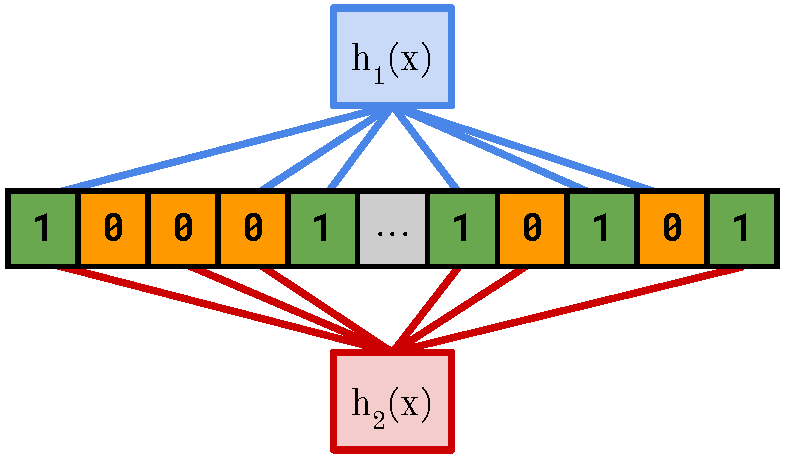
\includegraphics[width=.4\textwidth,center]{scoring/ECFP+RF}
  \caption{Example of a random forest with two learners\\using a fingerprint representation}
  \label{fig:ecfp+rf}
\end{figure}

\Fig{ecfp+rf} gives an example of the algorithm. The two weak learners $h_1$ and $h_2$ (both regression trees) observe different bits in the fingerprint representation of the molecule, and offer their prediction. The (full) learner takes these weak outputs into account to produce a more robust prediction.

Using random forests in conjuction with fingerprints often provides the best predictor in the single task setting, where the scarcity of data forbids the use of more complex methods such as deep learning. However, it cannot learn accross tasks.


\subsubsection{Deep learning and drug discovery}

Following breakthroughs in domains including computer vision, autonomous driving, and natural language processing, deep learning methods have entered the domain of pharmaceutical research and development. Recent successes include the deconvolution of biological targets from omics data \citep{min2017deep}, generation of drug-like compounds via \textit{de novo} molecular design \citep{xu2019deep}, and chemical synthesis planning \citep{segler2017neural, segler2017learning}.

A common characteristic of these applications, however, is the availability of high quality data, and in high quantities.
Unfortunately, many critical prediction tasks in the drug discovery pipeline fail to satisfy these requirements, in part due to resource and cost constraints \citep{cherkasov2014qsar}.

The lack of abundant and clean data certainly explains why deep learning is still relatively stealth in the worl of drug discovery and more particularly scoring. To be able to use more expressive (and thus more data-hungry) models, we need to find a way to provide them with more training data.



% \subsection{Generation}







\clearpage
\section{Learning from multiple tasks}

As we have established in \sect{low-data}, the main issue computational biochemists need to tackle is the limited availability of examples. Yet, although data is indeed scarce for each biochemical property, the number of bioassays is in fact enormous. Moreover, we make the assumption that some amount of structural information can be shared between tasks.

Imagine you’re first learning to recognise cats from dogs, and then birds from zebras. In the traditional machine-learning pipeline, you would simply discard everything you learned from the first task, even though it is quite easy to realize that the problems share a lot of information: for instance, the low-level features such as edge and shape detection learnt in the first task can be used in the second one with minimal adaptation.

Transpose the issue to drug discovery, where training data is painfully scarce, and you’re looking at catastrophic underperformance if you naively apply the traditional machine-learning methodology. Indeed, the vast majority of biochemistry assays only come with a few tens of examples, which makes using the knowledge acquired across a number of distinct tasks all the more important.

Hence, methods have been developed to cope with the lack of data for individual assays by capturing knowledge from multiple tasks directly. I will discuss two solutions:
\begin{enumerate}
  \item \textit{Multi-task learning}, where a model is trained to output a vector that predicts the activity for every tasks at once.
  \item \textit{Meta-learning}, a radically different approach where the model is explicitly trained to learn new problems faster (ie with fewer datapoints).
\end{enumerate}



\subsection{Multi-task learning}
\label{sec:multitask}

Multi-task learning is the first step to benefit from the knowledge shared across tasks. It is very much a traditional machine-learning technique, but uses clever tricks to learn from multiple tasks at once.

The idea is simple: instead of learning to perfom each task individually, we consider only one multi-dimensional regression problem. Once again, let $x$ be the representation of a given molecule. Let $y_t$ denote its activity related to the $t^\text{th}$ task; note that this information may not be available to us since all molecules are not tested in each bioassay. We can define $\vy$ to be the concatenation of those targets, with the convention of setting to zero the missing labels:
\begin{equation}
  \vy = (y_1, y_2, \dots, y_n) \qquad \text{and} \qquad \hat{\vy} = (\hat{y}_1, \hat{y}_2, \dots, \hat{y}_n)
\end{equation}
The machine-learning problem now amounts to predicting the entire vector of activities. By transforming the task that way, we can exploit the hundreds of thousands of examples and training a deep learning algorithm using back-propagation becomes possible.

But there is one piece missing: we do not want to propagate the error on a target that we abitrarily set to zero. The trick is to keep track of the task index and only consider the corresponding component for each training example.

\begin{figure}[ht]
  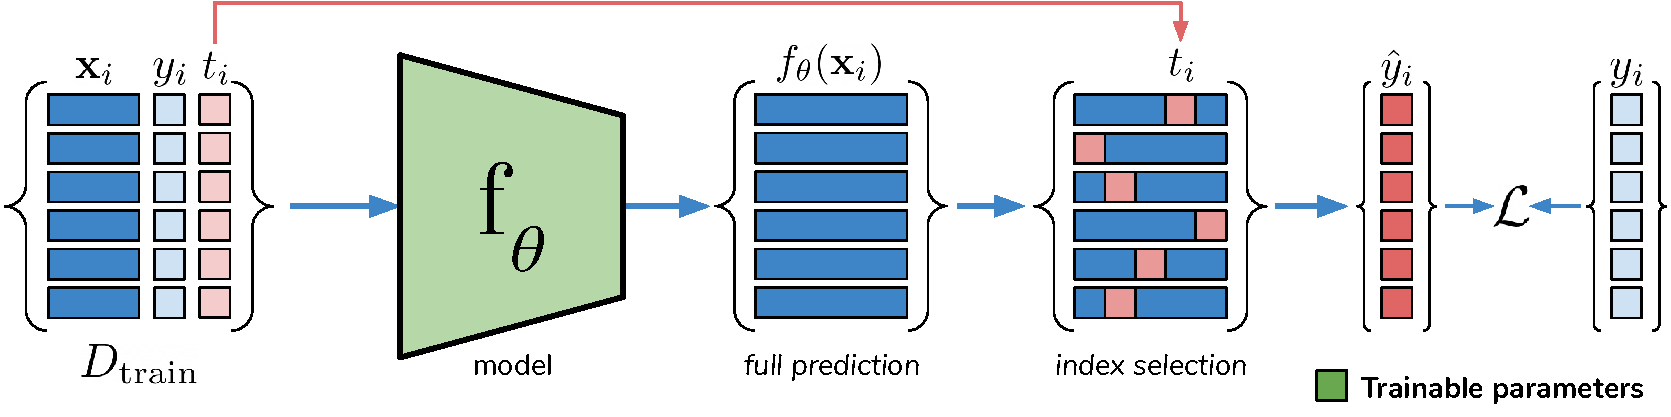
\includegraphics[width=.9\textwidth,center]{scoring/multitask}
  \caption{Diagram of a multi-task model}
  \label{fig:multitask}
\end{figure}

\Fig{multitask} shows how the multi-task model is adapted to work in a setting where some targets are missing. The network is trained to output the full prediction vector, but only the component that corresponds to the considered bioassay is compared to the target. That way, we propagate an error signal using every single training example.

More formally, the optimisation problem associated with this method is:
\begin{equation}
  \label{eq:multitask}
  \argmin_\theta \quad \E_{x, t, y \in \Dtrain} \LB \loss (y, f_\theta(x)_t) \RB
\end{equation}
Where $t$ is the index of the task. Note that a single molecule may appear multiple times in the training dataset should it have been tested in different bioassays.

Multi-task learning is a first step towards learning across task, using a natural idea that adapts traditional methods. However, this family of algorithms is still not particularly well-suited for few-shot learning. That is especially true in a drug discovery setting, where we would perform preliminary \textit{in vitro} testing for a new property and expect the algorithm to generalise well such that it may guide the molecular search efficiently.

In other words, multi-task learning focuses on learning from multiple tasks in parallel. It can still construct a better representation of molecules in the intermediate layers, since that latent encoding is specifically designed to perform well on a variety of tasks. It has however a limited effectiveness when a new task comes along, a common case in the world of drug discovery.


\subsection{Meta-learning}

A new range of algorithms has been developed in recent years in order to tackle the issue of generalising from very few examples (what is known as few-shot learning). The field, called meta-learning, aims at ``learning to learn'' from a collection of machine-learning problems that share a substantial amount of structure.
The crux of meta-learning is to design the objective function in such a way that the algorithm is explicitly trained to learn faster.

In what follows, I will first discuss the vocabulary and notations that surround this relatively new field. Then, I will insist on the objective function and show how it leads the algorithm to \textit{learn how to learn}. Finally, I will present some methods from the discipline and focus on what is arguably the most popular meta-learning algorithm, namely model-agnostic meta-learning or MAML.

MAML serves as a great pedagogical tool when it comes to presenting meta-learning, since it examplifies particularly well what is expected to be learnt in that paradigm.


\subsubsection{Vocabulary and notations}

If you come from a traditional machine-learning background, meta-learning can be mildly confusing at first, and the vocabulary does not help.

Unlike the traditional machine-learning setting where you want to train a model on a distribution of individual examples $p(x)$, in meta-learning we train an algorithm to learn as fast as possible when presented a new task $t \sim \tau(t)$. However, we do not have access to either $p(x)$ or $\tau(t)$: as an alternative, we use a dataset assumed to have been sampled from that distribution.

\begin{table}[ht]
  \centering
  \begin{tabular}{@{}lll@{}}
    \toprule
    & Traditional machine-learning &  Meta-learning \\
    \toprule
    \multirow{2}{*}{Input} & Training set $\Dtrain$: &  Meta-training set $\Dmtrain$: \\
    & $\Dtrain = \LC (\vx_i, y_i) \RC$ & $\Dmtrain = \LC (\Dsupport, \Dquery) \RC_{t \in T}$ \\
    \midrule
    Output & Model parameters &  Meta-model parameters \\
    \midrule
    \multirow{2}{*}{Objective} & Minimise generalisation error &  Minimise generalisation error\\
    & on the test set & on $\Dquery$s from meta-test set\\
    \bottomrule
  \end{tabular}
  \caption{Comparison of traditional machine-learning and meta-learning}
  \label{tab:metaml}
\end{table}

In meta-learning, we work with a \textit{collection of datasets}, each representing one given task –and containing individual examples from it. The collection is divided into a meta-training set $\Dmtrain$ and a meta-test set $\Dmtest$, and its datasets are each separated between training and test sets.

To limit confusion in the meta-learning setting, each task within the meta-collection will be divided between \textit{support} and \textit{query} sets to avoid over-using the \textit{training} and \textit{test} vocabulary, which will be restricted to the separation of the tasks.
Hence:
\begin{equation*}
  \Dmtrain = \LC \LC \Dsupport, \: \Dquery \RC \RC_{t \in T_\text{train}} \quad \text{and} \quad
  \Dmtest = \LC \LC \Dsupport, \: \Dquery \RC \RC_{t \in T_\text{test}}
\end{equation*}



\subsubsection{The meta-objective}

In the meta-learning setting, we train algorithms to \textit{learn how to learn} from a variety of tasks that share some amount of structural information. The purpose of the training procedure is to teach the model to adapt as fast as possible to each task using the support set, in order to optimise the generalisation performance on the query set. More formally, a meta-learning algorithm aims to optimise the following minimisation problem:
\begin{equation}
  \label{eq:maml}
  \argmin_\theta \E_{t \in \Dmtrain} \LB \metaloss (\Dquery \mid \theta, \Dsupport) \RB
\end{equation}
where $\metaloss$ denotes the full loss and $\metaloss (\Dquery \mid \theta, \Dsupport)$ the meta-loss on the support set after adaptation.

More specifically, letting $\theta'$ be the parameter adapted on $\Dsupport$:
\begin{equation}
  \metaloss (\Dquery \mid \theta, \Dsupport) = \sum_{\vx, y \in \Dquery} \loss (f_{\theta'}(\vx), y)
\end{equation}

 % $\metaloss (\Dquery \mid \theta, \Dsupport)$ is the full loss recorded on the query set after adaptation on the support set.

At first glance, a few details may worry the layman in meta-learning. To wit, the approach is all about back-propagating (or more generally, minimising) the error on the \textit{test set}, which raises a major red flag in the traditional machine-learning setting.

But there is no contradiction, nor is there a leak of information. Indeed, the goal of meta-learning is to learn as fast as possible on \textit{new tasks}.
Instead of learning on a distribution of examples, represented by the datasets $\Dtrain$ and $\Dtest$, a meta-learning algorithm learns to adapt quickly within a \textit{distribution of tasks}.
% , represented by $\Dmtrain$ and $\Dmtest$.


\begin{wrapfigure}[16]{l}[1.25cm]{0.45\textwidth}
  % \vspace{-.25cm}
  \centering
  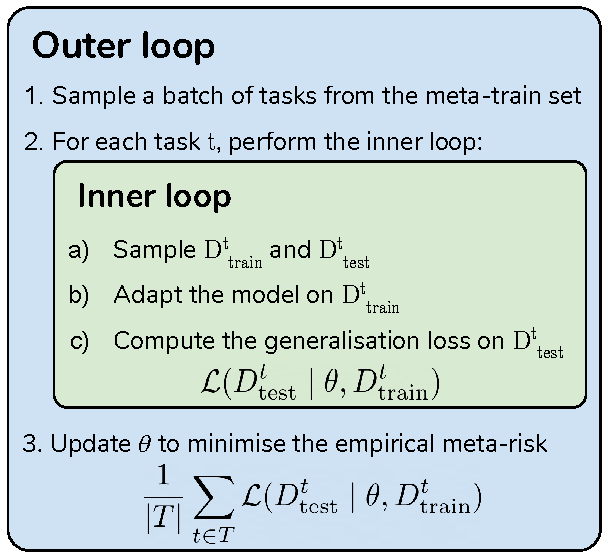
\includegraphics[width=.95\linewidth]{scoring/metaml}
  \caption{The general\\meta-learning algorithm} % \\(here with a gradient-based learning rule)}
  \label{fig:metaml}
\end{wrapfigure}

% \begin{figure}[ht]
%   \centering
%   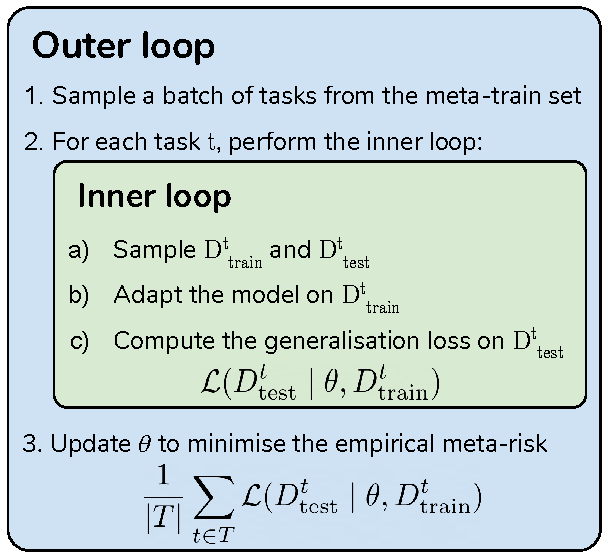
\includegraphics[width=.4\linewidth]{scoring/metaml}
%   \caption{The general\\meta-learning algorithm} % \\(here with a gradient-based learning rule)}
%   \label{fig:metaml}
% \end{figure}

Perhaps a more intuitive way to look at meta-learning is to understand that the training procedure (depicted in \fig{metaml}) is divided between an inner-loop, where the algorithm \textit{adapts} to a new task, and the outer-loop, where the algorithm \textit{learns} how this adaptation could be better-performed. At test time, only the inner loop is performed on a previously unseen task.

In \fig{metaml}, I present the general training procedure behind meta-learning. It is worth noting that most meta-learning algorithms are trained in the so-called ``episodic'' setting, where the support and query sets are subsampled during training to remain in the few-shot learning regime, hence the sampling operation in the inner-loop. That operation is often left out at test time, since limiting the number of support examples would likely hurt the generalisation performance\footnote{Performance decrease is likely but not automatic: the meta-learning algorithm is trained in a few-shot regime and as we deviate from it, performance may decrease before ultimately going up again.}.


% \begin{figure}[ht]
%   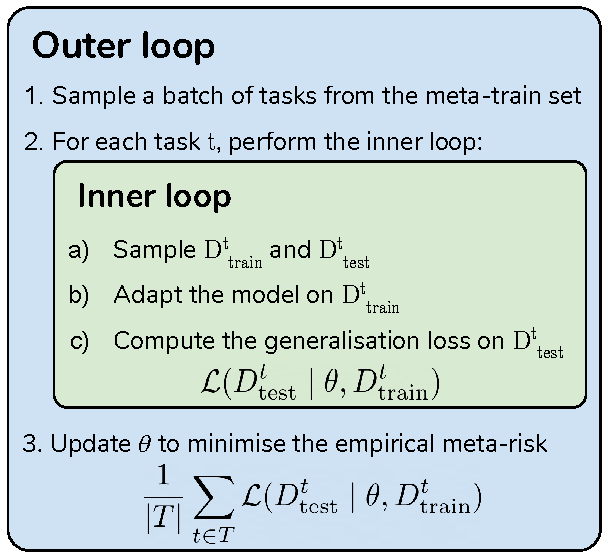
\includegraphics[width=.4\textwidth,center]{scoring/metaml}
%   \caption{The meta-learning algorithm\\(here with a gradient-based learning rule)}
%   \label{fig:metaml}
% \end{figure}

% To limit figure fig:metaml from overstepping on the next page.
% \clearpage

Both the adaptation and the meta-loss minimisation can be performed in a number of ways, and numerous methodology have been proposed. In what follows I will focus on one algorithm in particular, model-agnostic meta-learning (MAML), since it has become a ubiquitous baseline achieving state-of-the-art results in a variety of tasks.


\subsubsection{Meta-learning methods}

Most meta-learning algorithms differ in two aspects:
\begin{itemize}
  \item The nature of the meta-knowledge, or information shared across tasks, captured;
  \item The amount of adaptation performed at test-time for new tasks or datasets.
\end{itemize}
In a drug discovery setting, due in part to the unfathomable size of the chemical space \citep{bohacek1996art}, we need methods that are expressive enough to allow extrapolation and uncertainty estimation in unseen regions of chemical space at test-time. What is more, a single molecule can have results be reported for multiple bioassays, which means test-time adaptation is particularly important.

Authors have proposed to use metric learning methods \citep{koch2015siamese, vinyals2016matching, snell2017prototypical, garcia2017few, bertinetto2018meta} for meta-learning.
Such techniques accumulate meta-knowledge in high capacity distance functions and use simple base-learners such as k-nearest neighbors \citep{snell2017prototypical, vinyals2016matching} or low capacity neural networks \citep{garcia2017few} to produce adequate models for new tasks. The idea is simple: we can afford to share a complex and expressive network, since it will be trained on all task and therefore on numerous examples, but the task-specific part needs to be as light as possible.
However, the covariance functions are not adapted at test-time.

Another avenue explored in recent years relates to initialisation- and optimisation-based methods \citep{finn2017model, kim2018bayesian, ravi2016optimization}.
These algorithms respectively learn the initialisation point and update rule for gradient descent-based algorithms, allowing them to adapt faster on new tasks –at the cost of necessitating slow and memory inefficient training.


\subsubsection{Model-agnostic meta-learning}
\label{sec:maml}

\begin{wrapfigure}[10]{r}[1.6cm]{0.4\textwidth}
  \centering
  \vspace{-.3cm}
  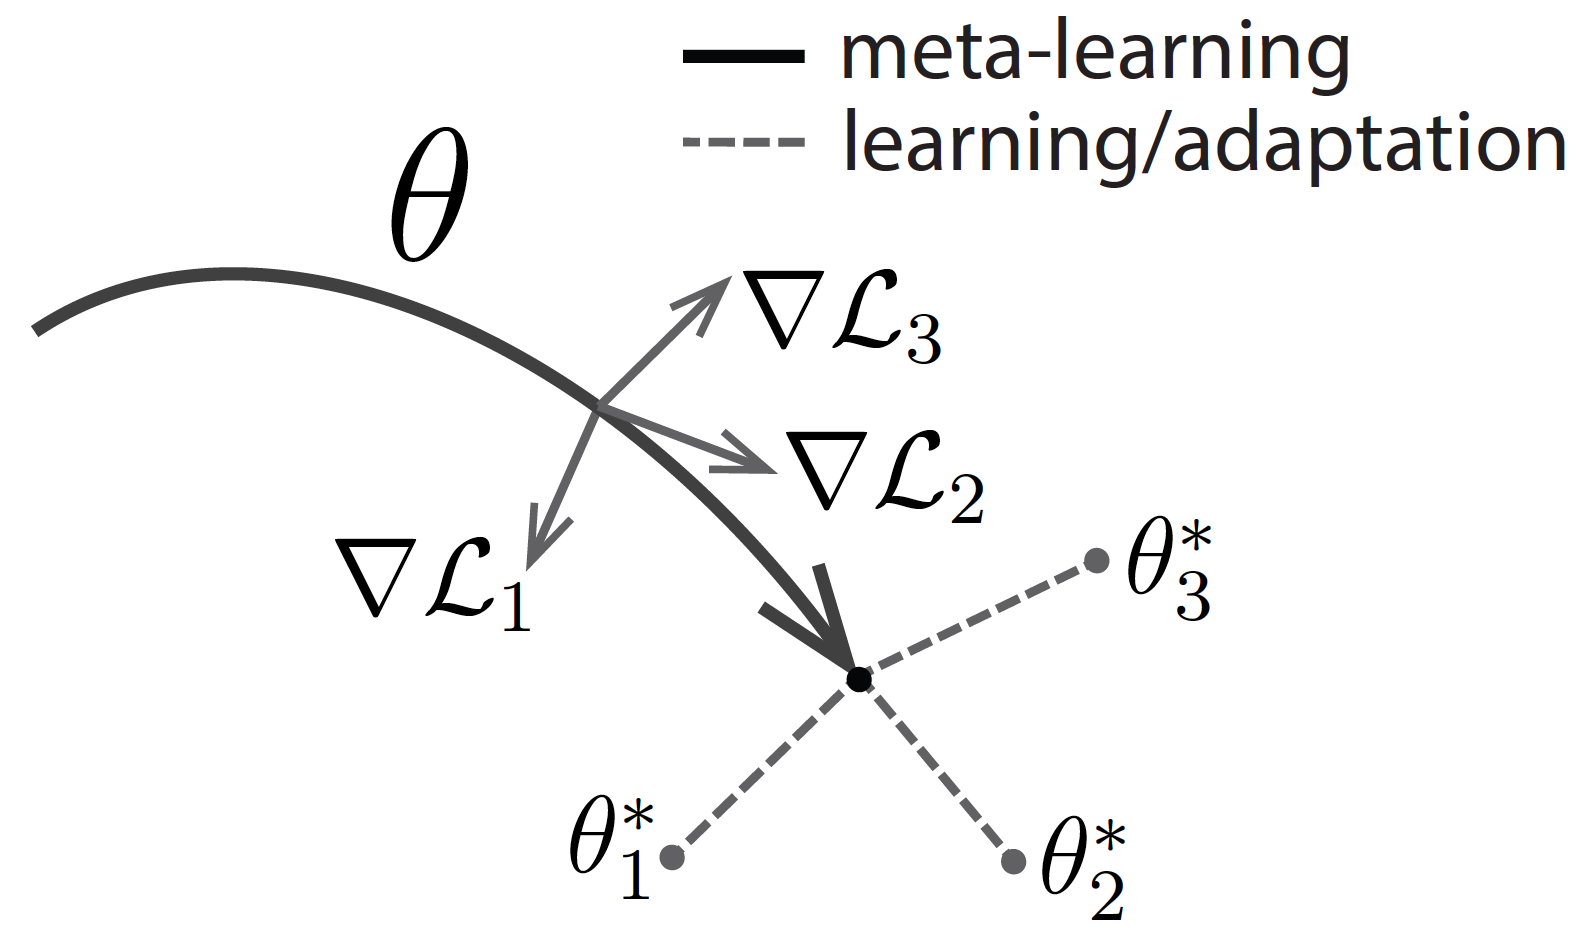
\includegraphics[width=.95\linewidth]{scoring/maml}
  \caption{Diagram of MAML\\\citep{finn2017model}} % \\(here with a gradient-based learning rule)}
  \label{fig:maml}
\end{wrapfigure}

Model-agnostic meta-learning \citep{finn2017model}, or MAML, is one of the most commonly used meta-learning method. Its popularity stems in part from the fact that it can adapt any differentiable machine-learning algorithm to meta-learning.

The approach, presented in \fig{maml}, is extremely straightforward: it looks for a parameter initialisation that enables the model to learn faster on new tasks, using gradient descent. Since gradient descent itself is differentable, MAML simply back-propagates the error on the query set through the gradient descent steps all the way to the ``initial parameters''.

More formally, let $f_\theta$ be a machine-learning model parametrised by $\theta$. MAML minimises the meta-objective described in \eq{maml} by optimising $\theta$ to reach better performance on average after adaptation, using the procedure presented in \algo{maml}.

\begin{algorithm}[ht]
  \caption{Model-Agnostic Meta-Learning \citep{finn2017model}}
  \label{algo:maml}
  \begin{algorithmic}[1]
    \REQUIRE $\tau(t)$: distribution over tasks
    \REQUIRE $\alpha$, $\beta$: step size hyper-parameters
    \STATE Randomly initialize $\theta$
    \WHILE{not done}
      \STATE Sample batch $T$ of tasks $t \sim \tau(t)$
      \FORALL{$t$}
        \STATE Sample support and query sets $\Dsupport$ and $\Dquery$
        \STATE Evaluate $\nabla_\theta \metaloss(\Dsupport \mid \theta)$ with respect to the support set
        \STATE Compute adapted parameters with gradient descent:
        $\theta_t=\theta-\alpha \nabla_\theta \metaloss(\Dsupport \mid \theta)$
      \ENDFOR
      \STATE Update $\theta \leftarrow \theta - \beta \nabla_\theta \sum_{t \in T}  \metaloss(\Dquery \mid \theta_t)$
    \ENDWHILE
  \end{algorithmic}
\end{algorithm}

Note that the procedure described by \algo{maml} requires a distribution over tasks. In practice, we do not have access to such a distribution; we can however make the assumption that the meta-datasets $\Dmtrain$ and $\Dmtest$ are sampled from $\tau(t)$.

As \algo{maml} illustrates, MAML is strikingly simple. It hinges on a simplistic idea: since we want our algorithm to learn more efficiently, let us just adjust the objective function to train for that explicitly. And seeing that gradient descent –the workhorse of vast majority of machine-learning algorithms today– is differentiable, \citeauthor{finn2017model} proposed a method that adapted virtually the entire field to meta-learning.

Being gradient-based, MAML presents the advantage of truly adapting to the new task at test time and in a principled manner, where some other methods merely learn huge representation networks in the hope of mitigating the effects of domain adaptation. Of course, it does have some drawbacks. For one thing, negative adaptation\footnote{Negative adaptation refers to the cases where the generalisation performance is worse off after adaptation. Being gradient-based, MAML should eventually reach a good local minimum after enough adaptation steps and examples.} remains possible and not yet well-understood \citep{deleu2018effects}. It is also painfully slow and resource-intensive to train, owing to the need to compute the Hessian of a gradient.

% So far, a method that is both relatively lightweight in terms of resources and still able to adapt in a meaningful manner at test time is elusive, and still very much an active avenue of research.

% \subsubsection{Task representation}
% \subsection{Generation}


\clearpage
\section{Adaptive deep kernel learning}

In the previous section, we saw two general paradigms to learn from more than one task. First, I presented  \hyperref[sec:multitask]{multi-task learning}, a natural step to adapt traditional machine-learning to a setting where multiple tasks are available for training. Then, I focused on a radically different strategy whose goal is to \textit{learn to learn efficiently}, hence its name: meta-learning.

% Describing one of the most used meta-learning methods, I pointed out the fact that intense research efforts are dedicated to discover a method that can unite proper test-time adaptation with smaller computational costs, a set of desiderata that have so far eluded the proposed methods.

As we have established in \sect{drug-discovery}, building methods apt to learn efficiently from very few datapoints is vital in a drug-discovery context. The field is particularly well-suited for a meta-learning approach: it advertises ample amounts of data, scattered into a myriad of different tasks. Making the reasonable assumption that molecular structure is at the root of the activity, and that we can use common patterns from one task to the other as a low-level representation, meta-learning becomes a natural research avenue to tackle computational drug discovery.

Striving to unleash the potential of artificial intelligence in the field of drug discovery, InVivo AI aims to develop novel methods that can learn from very few datapoints, and we actively explore the route of meta-learning, leading to novel methods being developed in-house as well as submissions to higher-tier publications and conferences.

In this section, I will focus on one such project on which I spent most of my time at InVivo AI, namely a novel framework we called Adaptive Deep Kernel Learning, or ADKL for short.
The ADKL family is a set of algorithms that can efficiently learn from a large collection of problems and generalise the gathered knowledge to new tasks.

That work was led with Prudencio Tossou, co-founder and head of research at InVivo AI (and my supervisor), along with Mario Marchand and François Laviolette from Université Laval as well as Alexandre Lacoste from Element AI, and with the help of Daniel Cohen, CEO and co-founder of InVivo AI.


\subsection{Desiderata and contributions}

Being a drug discovery company, InVivo AI focuses on modelling bioassays, specifically those relevant in the early stages of drug discovery: primarily binding and cellular readouts. Data from these assays, consisting of libraries of molecules and their associated real-valued activity scores, is often extremely small and noisy (see \append{collections-real} for an eloquent demonstration of that issue).

As we have seen in \sect{drug-discovery}, data collected in bioassays are not only scarce but also incredibly specific\footnote{Examples of specific assays include testing the antibacterial effect on a given strain of bacterium, in presence of a particular adjuvant...}, owing to the combinatorial nature of possible test configurations. That specificity makes it impossible to compare data collected across different assays directly.

% To tackle the formidable challenge of drug discovery, it is obvious that robust few shot learning algorithms are needed.

Furthermore, bioassay modelling is intended to be the first step in a full drug discovery pipeline, that will eventually include direct molecular optimisation (e.g. with Bayesian optimization) and efficient exploration of the chemical space (e.g. active learning). Hence, accurate prediction and uncertainty estimation using few datapoints is critical to successful downstream applications in drug discovery.

% Let us recapitulate the desiderata for drug-discovery ready learning algorithm:
% \begin{enumerate}[noitemsep]
%   \item Aptitude to learn across tasks;
%   \item Coping with scarce, heterogeneous and noisy data;
%   \item Well-calibrated uncertainty;
%   \item Ability to incorporate domain-specific expert knowledge.
% \end{enumerate}

% During this project, the research team at InVivo AI and I worked to propose a framework that can learn across task, cope with scarce and heterogeneous data, that has well-calibated uncertainty, and can incorporate expert knowledge.

In \href{https://openreview.net/pdf?id=Syeu8CNYvS}{the paper we submitted}, our contributions were three-fold. First, we framed few-shot regression as a deep kernel learning (DKL) problem and demonstrated its advantages relative to classical metric learning methods.
Then, we derived the ADKL framework by learning a task-dependent kernel, allowing for more test-time adaptation than the DKL framework.
Finally, we introduced two real-world datasets for modelling biological assays.


\subsection{Deep kernel learning}

As the name suggests, ADKL is part of the family of kernel methods. In simple words, that means that in order to make a prediction about a new molecule, the algorithm will compare that compound to the labelled examples seen in the support set. We call it ``deep'' kernel learning because ADKL uses a deep network to create a representation of the compounds which makes this comparison easier.

Recall that meta-learning algorithms can be roughly divided into two families: those that store meta-knowledge in an extremely expressive network that is common to all tasks but limit the amount of task-adaptation at test time, and those that do adapt to the new task at the cost of slower and more resource-intensive training.

Working on ADKL, we were looking to make a step towards combining the strengths of both types of methods, a crucial feature to be able to score molecular compounds efficiently. For that reason, we chose to frame the bioassay modelling task as a deep kernel learning problem.


\subsubsection{Overview of the method}

Before I present the adaptive deep kernel learning method itself, let us first dive into the deep kernel learning (DKL) framework.

\begin{figure}[ht]
  % \vspace{1cm}
  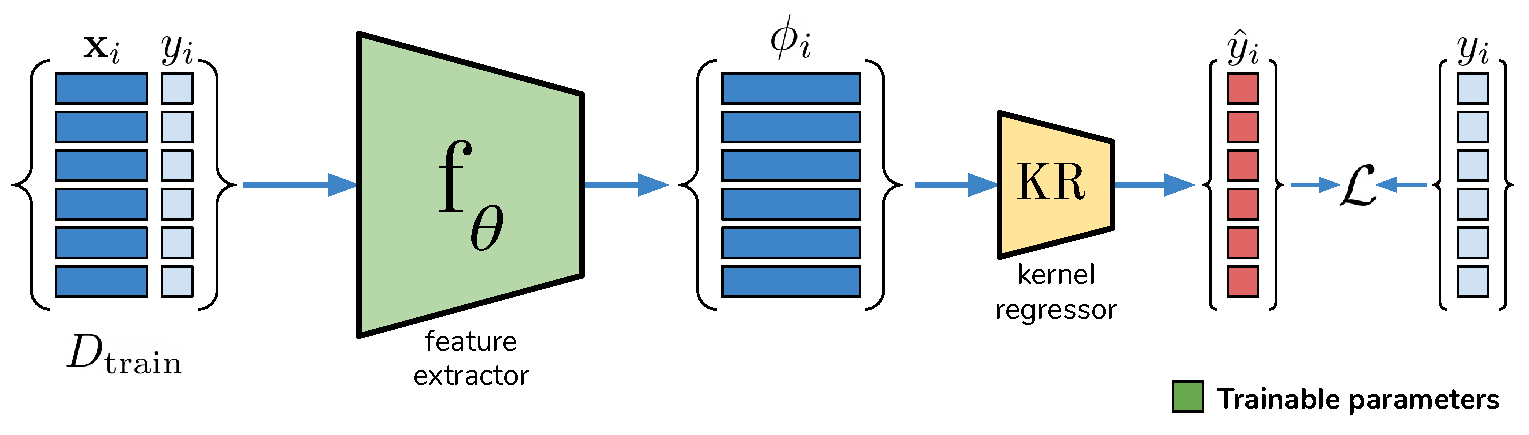
\includegraphics[width=.9\textwidth,center]{adkl/dkl}
  \caption{Diagram of the deep kernel learning framework}
  \label{fig:dkl}
\end{figure}

\Fig{dkl} shows a diagram of the deep kernel learning method. DKL is not specifically designed for meta-learning, and was developed long before few-shot learning became an issue. Once again, the intuition behind the framework is simple: the goal is to train a large feature extractor network, whose role is to transform inputs into a meaningful representation that can then be used by a kernel method such as kernel Ridge regression (KRR).

\clearpage
The deep kernel learning algorithm consists of two parts:
\begin{enumerate}
  \item The feature extractor $f_\theta$, the only trainable section of the algorithm. It performs a non-linear mapping of the inputs into an embedding where the representation is trained to be more meaningful for the machine-learning problem;
  \item The kernel regressor $\kr$. Not trainable (it merely records the training examples), it outputs a prediction based on the distance between each examples.
\end{enumerate}
As long as the kernel method itself is differentiable, we can back-propagate the empirical risk on the training set through the kernel to the parameters of the feature extractor.

Candidate kernels include the radial basis, polynomial, and linear kernels. Kernel Ridge regression (KRR) and gaussian processes (GP) are two popular and differentiable kernel methods that can be plugged onto the deep kernel learning framework.

Let $\km$ represent the kernel map: $\km_{\vu, \vv} = \kernel(f_\theta(\vu), f_\theta(\vv))$. Let $\vy$ represent the stacked labels for the training set.
% For brevity, I will use $\km_{\mathrm{train} \times \mathrm{train}}$ and $\km_{\mathrm{train} \times \mathrm{train}}$ as the kernel map between the training and test set and the training set.

\paragraph{Kernel Ridge regression} KRR minimises the mean squared error of the training prediction, penalising the $L^2$ norm of the regressor: $\argmin_{\va} \lambda \norm{\va}^2 + \norm{\km_{\mathrm{train} \times \mathrm{train}} \cdot \va - \vy}^2$. Its prediction is in the form:
\begin{equation*}
  \kr^*(\vx') = \km_{\vx' \times \mathrm{train}} \cdot \va^* \quad \text{where} \quad \va^* = (\km_{\mathrm{train} \times \mathrm{train}} + \lambda \Id)^{-1} \vy
\end{equation*}

\paragraph{Gaussian process} When using the negative log likelihood loss function, the GP algorithm gives a probabilistic regressor in the form $\mathrm{GP}(\vx') = \calN(\mu, \Cov)$. Assuming a normal observation noise of standard deviation $\sigma$, the predictive mean $\mu$ and the covariance $\Cov$ are given by:
\begin{align*}
  \mu &= \km_{\mathrm{test} \times \mathrm{train}} \cdot (\km_{\mathrm{train} \times \mathrm{train}} + \sigma^2 \Id)^{-1} \vy \\
  \Cov &= \km_{\mathrm{test} \times \mathrm{test}} - \km_{\mathrm{test} \times \mathrm{train}} (\km_{\mathrm{train} \times \mathrm{train}} + \sigma^2 \Id)^{-1} \km_{\mathrm{train} \times \mathrm{test}}
\end{align*}

Note that in both cases, the predictor is obtained through a differentiable procedure, which means the feature extractor can indeed be optimised during training. However, it does necessitate the full kernel map $\km$, which can become cumbersome to compute should we have a large training dataset.

% Moreover, although I have omitted the hyper-parameters of the kernel, they might exist: in the case of the radial basis function for instance, it would be the bandwidth.

All in all, the deep kernel learning framework offers a way to drastically increase the expressivity of principled methods that otherwise present nice generalisation properties.

\subsubsection{Deep kernel learning for meta-learning}
\label{sec:dkl-meta}

It turns out that deep kernel learning can be adapted to meta-learning very easily. In the few-shot learning setting, we can share the feature extractor across task, while differentiating the last layer. Since DKL uses a regressor that is already task-specific, there is not much work to do!

\Fig{dkl-meta} illustrates the minor changes done to the algorithm to be ``meta-learning-ready''. Notice that we went from a single to a double track: one for training, and the other to test the generalisation performance on examples from the same task. Remember, in meta-learning we are interested in the minimisation of the generalisation error.
There is still a meta-test set, there to make sure that the algorithm performs well on completely new tasks.

\begin{figure}[ht]
  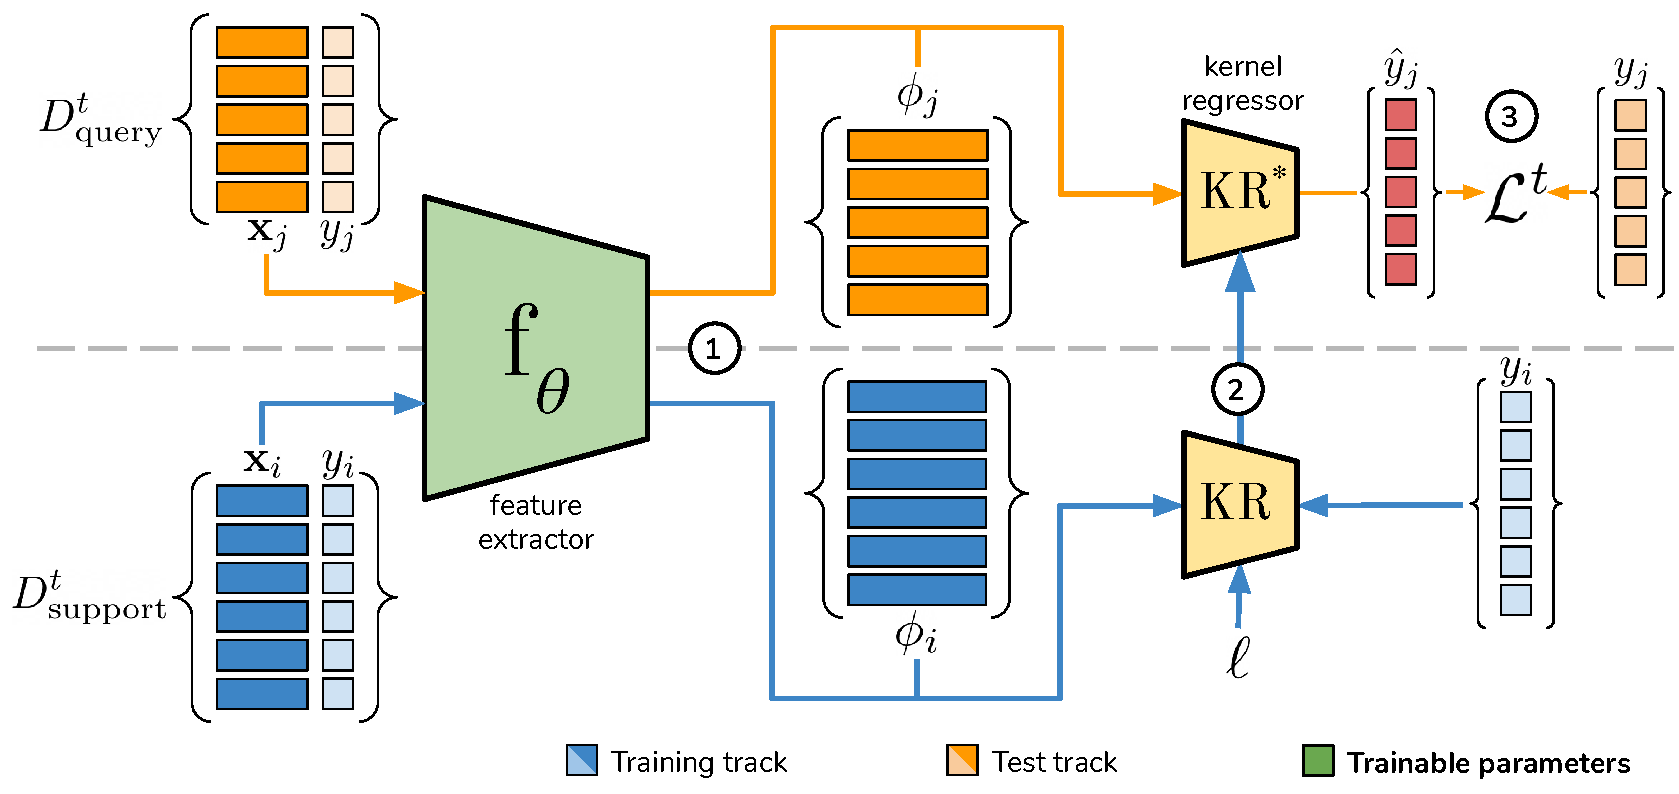
\includegraphics[width=.9\textwidth,center]{adkl/dkl-meta}
  \caption{Diagram of the adaptive deep kernel learning framework}
  \label{fig:dkl-meta}
\end{figure}

The procedure depicted in \fig{dkl-meta} is also described more formally in \algo{dkl}.

\begin{algorithm}[ht]
  \caption{Deep kernel learning for meta-learning}
  \label{algo:dkl}
  \begin{algorithmic}[1]
    \REQUIRE $\tau(t)$: distribution over tasks
    \REQUIRE Model hyper-parameters
    \STATE Randomly initialize $\theta$
    \WHILE{not done}
      \STATE Sample batch $T$ of tasks $t \sim \tau(t)$
      \FORALL{$t$}
        \STATE Sample support and query sets $\Dsupport$ and $\Dquery$
        \STATE 
\includegraphics[height=.35cm]{adkl/numbers/1} Map support and query sets to the latent space $f_\theta(\Dsupport)$ and $f_\theta(\Dquery)$
        \STATE 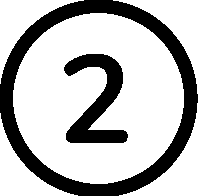
\includegraphics[height=.35cm]{adkl/numbers/2} Get the kernel regressor $\kr^*$ from $f_\theta(\Dsupport)$
        \STATE 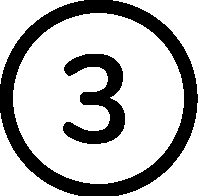
\includegraphics[height=.35cm]{adkl/numbers/3} Compute the generalisation error $\metaloss(\Dquery \mid \kr^* \circ f_\theta)$
      \ENDFOR
      \STATE Update $\theta$ to minimise the objective $\frac{1}{|T|} \sum_{t \in T}  \metaloss(\Dquery \mid \kr^* \circ f_\theta)$
    \ENDWHILE
  \end{algorithmic}
\end{algorithm}

% Recall the optimisation problem solved by regular DKL:
% \begin{equation}
%   \argmin_\theta \E_{\vx, y \in \Dtrain} \LB \loss(\kr^*(f_\theta(\vx)), y) \RB
% \end{equation}
%
% Since DKL uses task-specific kernel regressor, that procedure is straightforward to adapt to the few-shot learning setting.

To summarise, few-shot DKL aims to find a representation common to all tasks such that the kernel method (in our case, GP and KRR) will generalise well from a small amount of samples. It is worth noting that in doing so, the method alleviates two of the main limitations of single task DKL:
\begin{enumerate}
  \item The scalability of the kernel method is no longer an issue since we are in the few-shot learning regime. Even with several hundred samples, the computational cost of embedding each example is usually higher than inverting the Gram matrix.
  \item The parameters are learnt across a potentially large amount of tasks and samples, providing the opportunity to learn a rich representation without overfitting.
\end{enumerate}

Despite shared characteristics with the metric learning framework, the few-shot deep kernel learning framework is more powerful and flexible.
It provides better task-specific adaptation due to the inference of the appropriate model using the kernel methods compared to shared model parameters in metric learning.

After meta-training, any task-specific model also inherits the generalisation guarantees of kernel-based models, and consequently increasing the number of shots for new tasks can only improve generalisation performance. Moreover, using kernel-based methods enables the incorporation of expert knowledge within the network by choosing user-specific kernel functions, which is also a major advantage of DKL over metric learning. For example, one could use periodic kernels in a regression task that relates to recurrent functions.

In the framework, the feature extractor does not get adapted at test time. Rather, DKL finds a mapping that work as well as possible for every task in the meta-training set, relying on the kernel regressor to obtain good downstream performance.


\subsection{Adaptive deep kernel learning}

The lack of adaptation at test time is a huge drawback for the deep kernel learning framework. Indeed, relying solely on an adequate feature mapping puts a huge burden on the embedding network, as it is tasked with finding a representation that works well in every case.

Consider the following example. Suppose that you are training a deep kernel learning algorithm to recognise (and complete) sine functions\footnote{It turns out that very task has become one of the most commonplace testbeds for few-shot regression (see \append{collections-synthetic}).}, when provided only a handful of examples. This task would be relatively simple for a human to perform: knowing that you are looking at a sine wave, a handful of datapoints is enough to have a good idea of the phase and pulsation of the function.
On the other hand, a meta-learning algorithm might struggle:
\begin{itemize}
  \item For a plain DKL algorithm with no adaptation capabilities, the task will be hard. It needs to figure out a way to spread inputs in a way that lets the kernel regressor make the correct prediction at test time, and thus on an unknown function.
  \item If your algorithm can adapt to the task, however, it is bound to perform better, having the tools to possibly recognise the characteristics of the sine wave, much like a human would do.
\end{itemize}

This is the intuition behind adaptive kernel learning framework: we aim to extend the desirable properties, the simplicity and the potential of deep kernel learning, by adding an adaptation component, such that our algorithm can explicitly adapt at test time.

% Fundamentally, ADKL differs from few-shot DKL by
% 1) having more flexibility in its kernel definition and
% 2) learning to produce task-specific kernel functions during the meta-training instead of using one defined by the user.

The crux of the task adaptation component resides in an additional network that learns a representation of the task itself, using the entire support set as input rather than individual examples. ADKL consists of three independent neural networks that I will indicate with $f_\theta$, $g_\theta$ and $h_\theta$ in what follows. The networks are different but I decided to use only $\theta$ to denote the parameters to limit overloading notations.

% We describe in more detail both the task encoding network $\psib_{\etab}$ and the network $c_{\rhob}$ responsible for computing the task-specific kernel below.

%It does so by learning how to represent tasks with the task encoding network $\psib_{\etab}$ and then how to leverage task embeddings to build task-specific kernels using a  multi-modal neural network $c_{\rhob}$.

% It does so by learning a task representation using a task encoding network $\psib_{\etab}$ and leveraging it to build task-specific kernels using a multi-modal neural network $c_{\rhob}$.
% More explicitly, given a task $t$, ADKL first computes a task embedding $\zb_t = \psib_{\etab}( D^t_{trn}) $ using its support set $D^t_{trn}$ and then it infers the adapted kernel with $c_{\rhob}$.
% We describe in more detail both the task encoding network $\psib_{\etab}$ and the network $c_{\rhob}$ responsible for computing the task-specific kernel below.

\begin{figure}[ht]
  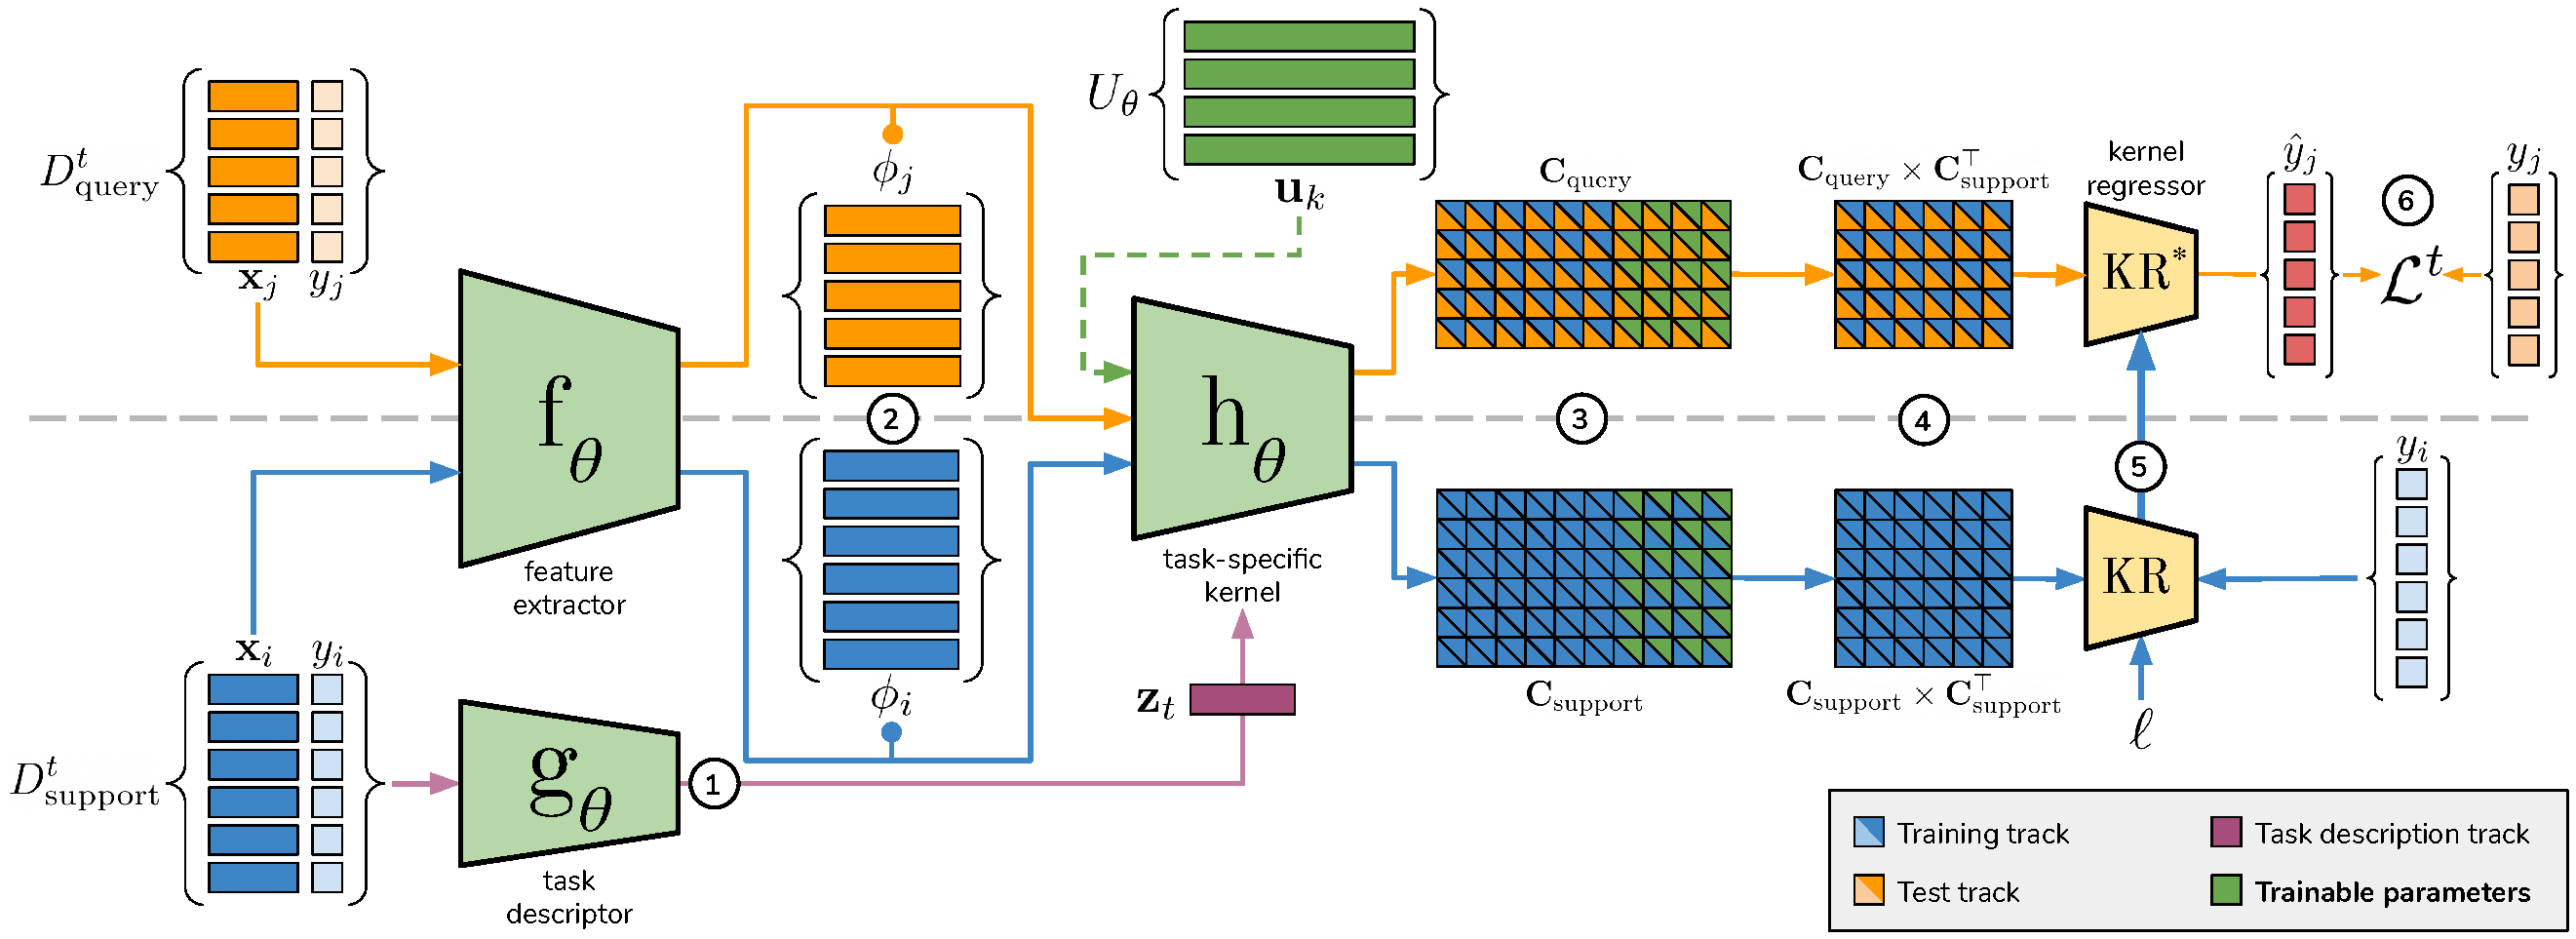
\includegraphics[width=1.35\textwidth,center]{adkl/adkl}
  \caption{Diagram of the adaptive deep kernel learning framework}
  \label{fig:adkl}
\end{figure}

\Fig{adkl} presents the architecture of the adaptive deep kernel learning framework. Let us go through the steps it depicts:
\begin{enumerate}[noitemsep]
  \item Given a task $t$, ADKL first computes a task embedding $\vz_t = g_\theta(\Dsupport)$.
  \item The method computes the feature embedding for both $\Dsupport$ and $\Dquery$, using the feature extractor $f_\theta$.
  \item The algorithm produces a task-specific kernel map of the datasets using $h_\theta$.
  % $h_\theta : \vx, \vx', \vz_t \mapsto \mathrm{MLP}(|\vx - \vx'|, \vz_t)$
  \item We use empirical kernel mapping to obtain positive semi-definite kernel, useable by the downstream kernel regressor.
  \item Using the support set and the choses kernel method, ADKL computes a regressor.
  \item The regressor is applied to the query set to get a prediction.
\end{enumerate}

In what follows, I will give more detail on the key steps of the adaptive deep kernel learning procedure.


\subsubsection{The task descriptor}

The challenge of the task descriptor network $g_\theta$ is to capture complex dependencies in the training set to provide a useful task encoding $\vz_t$.
That network should be invariant to permutations of the training set and be able to encode a variable amount of samples.
After exploring a variety of architectures, we found that more complex solutions, such as Transformers \citep{vaswani2017attention}, tend to underperform –possibly due to overfitting or the sensitivity of training such architectures.

\begin{figure}[ht]
  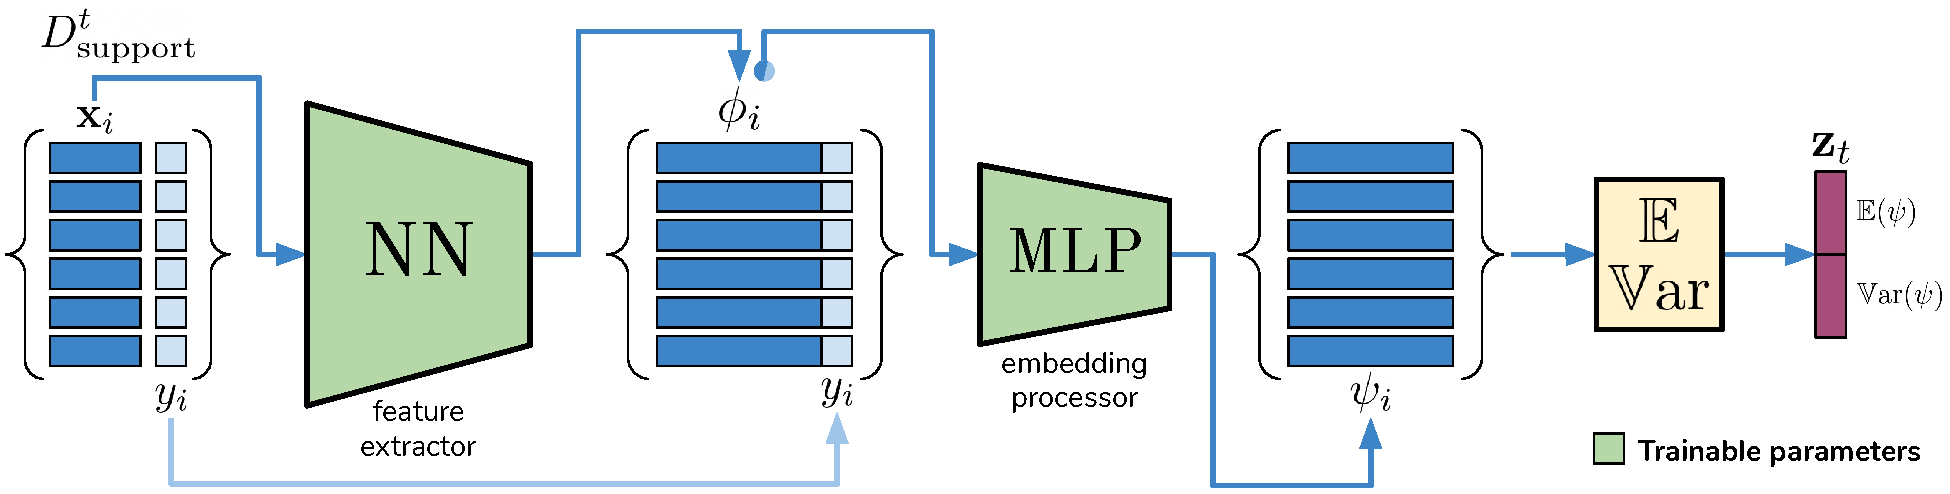
\includegraphics[width=.95\textwidth,center]{adkl/task-descriptor}
  \caption{Diagram of proposed task descriptor}
  \label{fig:task-descriptor}
\end{figure}

Consequently, inspired by the work on ``DeepSets'' by \citet{zaheer2017deep}, we propose a simple order invariant network that captures the first and second order statistics of regression datasets.
The procedure of the proposed method, presented in \fig{task-descriptor}, is as follows. Given a dataset $\Dsupport$, the network:
\begin{enumerate}[noitemsep, label=\alph*)]
  \item processes the samples individually via a neural network module (NN);
  \item concatenates input features with the target and embed the obtained vector using a simple multi-layer perceptron (MLP) model;
  \item computes the element-wise first and the second order statistics of the results, and concatenates them to produce the representation.
\end{enumerate}

More formally,
\begin{align}
  \vz_t &= \mathrm{Concat} \LB \mu_t, \sigma_t^2 \RB & &\text{with} & \mu_t &= \E_\Dsupport \LB \psi \RB & \sigma_t^2 &= \Var_\Dsupport \LB \psi \RB \\
  & & & \text{where} & \psi_i &= \mathrm{MLP}_\theta(\mathrm{Concat}\LB \phi_i, y_i \RB) & \phi_i &= \mathrm{NN}(\vx_i)
\end{align}
% \begin{align*}
%   && \vz_t &= \mathrm{Concat} \LB \mu_t, \sigma_t^2 \RB &&& \numberthis\\
%   &\text{with} & \mu_t &= \E_\Dsupport \LB \psi \RB & \sigma_t^2 &= \Var_\Dsupport \LB \psi \RB \\
%   &\text{where} & \psi_i &= \mathrm{MLP}(\mathrm{Concat}\LB \phi_i, y_i \RB) & \phi_i &= \mathrm{NN}(\vx_i)
% \end{align*}
using the same notation as \fig{task-descriptor}. The variance operator is applied element-wise.

During training, the task descriptor sees only one example per task, compared to the other parts of ADKL which are trained on batches of samples for each task. Hence, training is significantly slower and less stable.
To help train the task descriptor, we add a regularisation term that maximises the mutual information between $g_\theta(\Dsupport)$ and $g_\theta(\Dquery)$.
This penalisation encourages the network to produce similar task encodings when presented different data partitions for a given task.
In practice, we maximize a lower bound on the mutual information between the task representations given by the support and the query sets \citep{belghazi2018mine}.

Using a batch $T$ of tasks and the cosine similarity $c$ as the similarity measure the between two task encodings, the lower bound $\widehat{\mathrm{MI}}$ is defined as:
% by \cref{eq:reg_task} and is the regularizer that we used to a have better task encoder.
\begin{equation}
  \widehat{\mathrm{MI}} \define \frac{1}{|T|} \sum_{t \in T} c(\vz_\mathrm{s}^t, \vz_\mathrm{q}^t)
  - \log \LB \frac{1}{|T|(|T| - 1)} \sum_{t \in T} \sum_{\substack{t' \in T\\t' \neq t}} \exp \LB c(\vz_\mathrm{s}^t, \vz_\mathrm{q}^{t'}) \RB \RB,
\end{equation}
where $\vz_\mathrm{s}^t$ and $\vz_\mathrm{q}^t$ are the task description for task $t$ computed on the support and query set respectively.
% \begin{align}\label{eq:reg_task}
%     \tilde{I}_{\etab} \eqdef \tfrac{1}{b} \sum_{j=1}^b c(\enc(D^{t_j}_{trn}),\enc(D^{t_j}_{val})) - \ln \tfrac{1}{b(b-1)} \sum_{j=1}^b \sum_{i\neq j} e^{c(\enc(D^{t_j}_{trn}),\enc(D^{t_i}_{val}))}
% \end{align}


\subsubsection{Task-specific kernel}

I just presented how the task descriptor that we propose is able to provide an encoding of the current task, as well as the solution we advocate to train it better, namely a regularisation that maximises the mutual information between the description in different partitions of the same dataset. One question remains: how does ADKL make use of that task description to adapt itself? The answer resides in the task-specific kernel.

In deep kernel learning, the kernel is chosen in advance, and the only way to help the network adapt to novel tasks is to increase the capacity of the feature extractor. With ADKL, to the contrary, the kernel is computed using a trainable network that takes the task descrition as input to explicitly adapt to the current task.

The approach we propose uses a multi-modal neural network $h_\theta$. Given a pair of input representations $\phi \define f_\theta(\vx)$ and $\phi' \define f_\theta(\vx')$ and a task encoding $\vz_t$, $h_\theta$ computes the input pair similarity parametrised by the task encoding as follows:
\begin{equation}
    h_\theta(\phi, \phi' \mid \vz_t) = \mathrm{MLP}_\theta \LP \mathrm{Concat} \LB \norm{\phi - \phi'}^2_\mathrm{element}, \vz_t \RB \RP,
\end{equation}
where $\norm{\cdot}^2_\mathrm{element}$ is the element-wise $L^2$ distance and $\mathrm{MLP}_\theta$ is a multilayer perceptron whose last layer is a single neuron, such that it returns a scalar value.

Notice that with this definition, $h_\theta$ is symmetric and stationary, meaning that the output only depends on the element-wise distance between $\phi$ and $\phi'$ (and the task description). However, the upstream processing makes the full ADKL pipeline non-stationary with respect to the actual inputs.
The task-specific flavour of the module comes in the most simplistic way, by concatenating the task representation to the input of the multi-layer perceptron network, insuring that the kernel will indeed adapt to the current task.

However, the output $\mathbf{C}$ of the network is not positive semi-definite (PSD) and cannot be directly used for downstream kernel regressors such as KRR and GP.
Therefore, we use empirical kernel mapping \citep{scholkopf1999input} to compute the task-specific PSD kernel $\km$ associated with a given task representation $\vz_t$ obtained from $\Dsupport$.

Moreover, using the empirical kernel map of $\mathbf{C}$ to compute $\km$ offers the opportunity to introduce \textit{pseudo-representations} that can improve the kernel evaluations, especially in low data settings.
To wit, instead of computing the empirical kernel map with regard to $f_\theta(\Dsupport)$ alone, we use $S \define f_\theta(\Dsupport) \cup U_\theta$ where $U_\theta$ is a trainable set of pseudo-representations.

The final kernel map becomes:
\begin{align}
  \km_{\mathrm{q} \times \mathrm{s}} &= \mathbf{C}_\mathrm{q} \times \mathbf{C}_\mathrm{s}^\top & \text{and} && \km_{\mathrm{s} \times \mathrm{s}} &= \mathbf{C}_\mathrm{s} \times \mathbf{C}_\mathrm{s}^\top
\end{align}
where
\begin{align*}
  \mathbf{C}_\mathrm{s} &= \LC h_\theta(\phi, \phi' \mid \vz_t) \RC_{\phi, \phi' \in f_\theta(\Dsupport) \times S} & \text{and} && \mathbf{C}_\mathrm{q} &= \LC h_\theta(\phi, \phi' \mid \vz_t) \RC_{\phi, \phi' \in f_\theta(\Dquery) \times S}
\end{align*}
The subscripts $\mathrm{s}$ and $\mathrm{q}$ stand for ``support'' and ``query'' respectively.

The number of pseudo-representations is  a hyper-parameter of ADKL (in our experiments we chose $|U_\theta| \in \LB 0, 50 \RB $) and the set of pseudo-representations $U_\theta$ is a learnable parameters that is shared across tasks and learned during meta-training.
To prevent them from collapsing into a single point during training and to ensure that they are well distributed in the feature space, we add a regularisation term ($D_U$) to the training loss function.

To introduce this regularisation term, let us consider $p$ and $q$ to be the distributions that generate the true input representations and the pseudo-representations, respectively.
We make the assumption that $p$ and $q$ are both multivariate Gaussian distributions with diagonal covariance matrices and have respective parameters ($\mu_{\phi}$, $\sigma_{\phi}^2$) and ($\mu_{U}$, $\sigma_{U}^2$).

The parameters of $p$ can be estimated using the running mean and variance of all input representations computed over batches of tasks.
Those of $q$ are estimated using $U$ directly.
Hence, we regularise $U$ to constrain $q$ to be as close to $p$ as possible, such that the pseudo-representation effectively map the representation space. To that end, we add a regularisation term that minimises the Kullback-Leibler (KL) divergence between $p$ and $q$:
\begin{equation}
    D_U = \mathrm{KL}(\calN(\mu_U, \sigma_U^2) \parallel \calN(\mu_{\phi}, \sigma_{\phi}^2))
\end{equation}
which has a closed-form solution since both distributions are Gaussian.

Hence, the full training objective for ADKL is:
\begin{equation}
  \argmin_\theta \E_{t \in \Dmtrain} \LB \metaloss^t - \gamma_\mathrm{task} \widehat{\mathrm{MI}} + \gamma_\mathrm{pseudo} D_U \RB
\end{equation}

The complete ADKL algorithm is described in \algo{adkl}, referencing the steps featuring in \fig{adkl}.

\begin{algorithm}[ht]
  \caption{Adaptive deep kernel learning}
  \label{algo:adkl}
  \begin{algorithmic}[1]
    \REQUIRE $\tau(t)$: distribution over tasks
    \REQUIRE $\gamma_\mathrm{task}$, $\gamma_\mathrm{pseudo}$, $|U|$: model hyper-parameters
    \STATE Randomly initialize $\theta$
    \WHILE{not done}
      \STATE Sample batch $T$ of tasks $t \sim \tau(t)$
      \FORALL{$t$}
        \STATE Sample support and query sets $\Dsupport$ and $\Dquery$
        \STATE 
\includegraphics[height=.35cm]{adkl/numbers/1} Compute the task representation $\vz_t \define g_\theta(\Dsupport)$
        \STATE 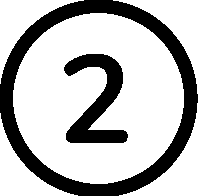
\includegraphics[height=.35cm]{adkl/numbers/2} Map support and query sets to the latent space $f_\theta(\Dsupport)$ and $f_\theta(\Dquery)$
        \STATE 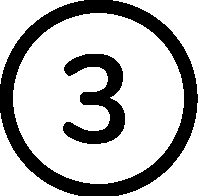
\includegraphics[height=.35cm]{adkl/numbers/3} Compute the task-specific kernel using $h_\theta$
        \STATE 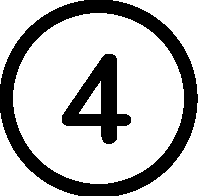
\includegraphics[height=.35cm]{adkl/numbers/4} Compute the empirical kernel maps
        \STATE 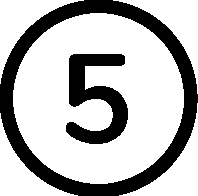
\includegraphics[height=.35cm]{adkl/numbers/5} Get the kernel regressor $\kr^*$ from $\km_{\mathrm{s} \times \mathrm{s}}$
        \STATE 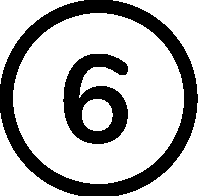
\includegraphics[height=.35cm]{adkl/numbers/6} Compute the generalisation error $\metaloss(\Dquery \mid \theta, \Dsupport)$
      \ENDFOR
      \STATE Update $\theta$ to minimise the objective $\frac{1}{|T|} \sum_{t \in T}  \metaloss^t  - \gamma_\mathrm{task} \widehat{\mathrm{MI}} + \gamma_\mathrm{pseudo} D_U$
    \ENDWHILE
  \end{algorithmic}
\end{algorithm}


\subsection{Experiments}

Now that we have looked at the theory behind ADKL, it is time to focuse on the actual performance of the framework.

To do that, we worked with three dataset collections. The first, \texttt{Sinusoids}, is synthetic. Initially proposed by \citet{kim2018bayesian}, it consists of a set of sine wave regression tasks: the model is provided five, ten or twenty samples from the $[-5, 5]$ interval, and is tasked with interpolating the function. The two other collections, \texttt{Binding} and \texttt{Antibacterial}, report real-world bioassay data coming from the public domain, and pre-processed by InVivo AI.

All three collections are presented in much more detail in \append{collections}, along with additional resource to access the datasets.

In the following paragraphs, I will first present the results of an ablation study that helped us understand the influence of the different hyper-parameters. Then, we will look at a benchmarking analysis to show how our framework compares to other meta-learning methods that I will introduce. Finally, we will focus on the active-learning capabilities of ADKL.

I will differentiate the kernel regressor used by the framework, using the denominations ``ADKL-KRR'' and ``ADKL-GP''. The former uses a kernel Ridge regressor while the latter implements a gaussian process estimator.

\subsubsection{Ablation study}

The role of the ablation study is paramount whenever a team proposes a new framework. Indeed, it is of the utmost importance that the community can assess the effect of the different hyper-parameters, particularly when the method introduces new ideas such as a task descriptor trained with mutual information.

Hence, we set out to closely evaluate the impact of the task encoder and the pseudo-inputs on the meta-generalisation error. We focused on the \texttt{Sinusoids} collection, since unlike the other two meta-datasets at our disposal, it provides a synthetic environment where the assumptions of meta-learning are entirely satisfied: we want to evaluate the impact of the parameters, not the flawed environment.

Thus, we trained and evaluated ADKL on \texttt{Sinusoids} with different hyper-parameter combinations.
\Fig{ablation} shows the relative improvements in the meta-test MSE compared to different baselines. The specific configurations can be found in \append{ablation}.

\begin{figure}[ht]
    \centering
    \begin{subfigure}[t]{0.72\textwidth}
        \centering
        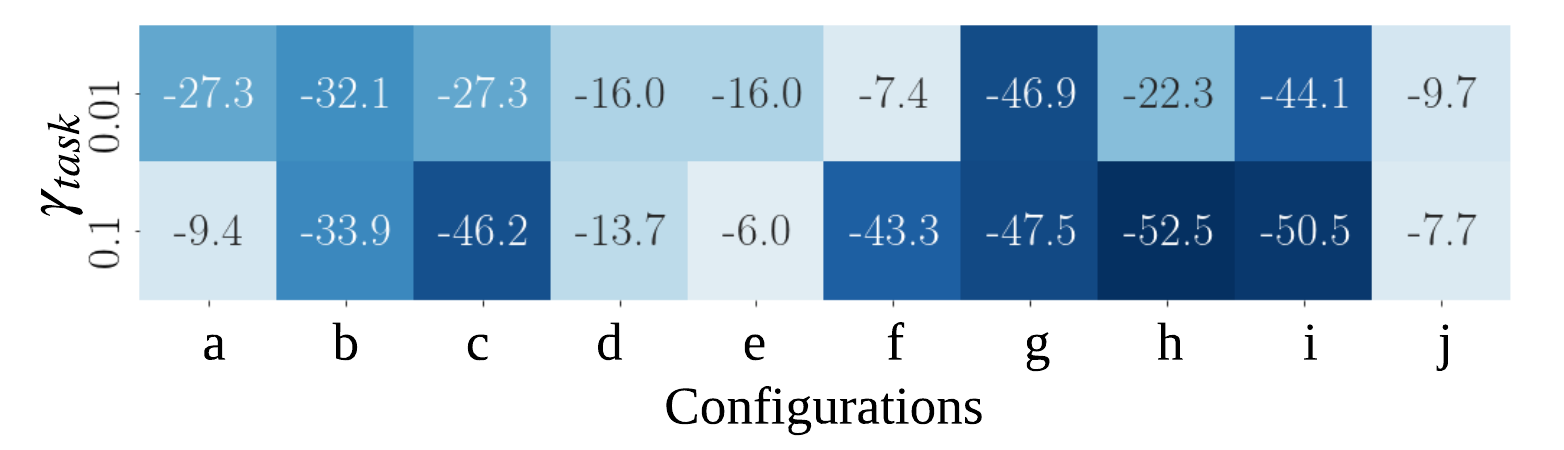
\includegraphics[width=\linewidth]{adkl/ablation/gamma-task}
        \caption{Impact of the task encoder trade-off parameter}
        \label{fig:gamma-task}
    \end{subfigure}
    \hfill
    \begin{subfigure}[t]{0.26\textwidth}
        \centering
        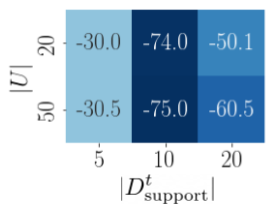
\includegraphics[width=\linewidth]{adkl/ablation/pseudo-krr}
        \caption{$|U|$ in ADKL-KRR}
        \label{fig:pseudo-krr}
    \end{subfigure}
    \vspace{0.2cm}
    \begin{subfigure}[t]{0.72\textwidth}
        \centering
        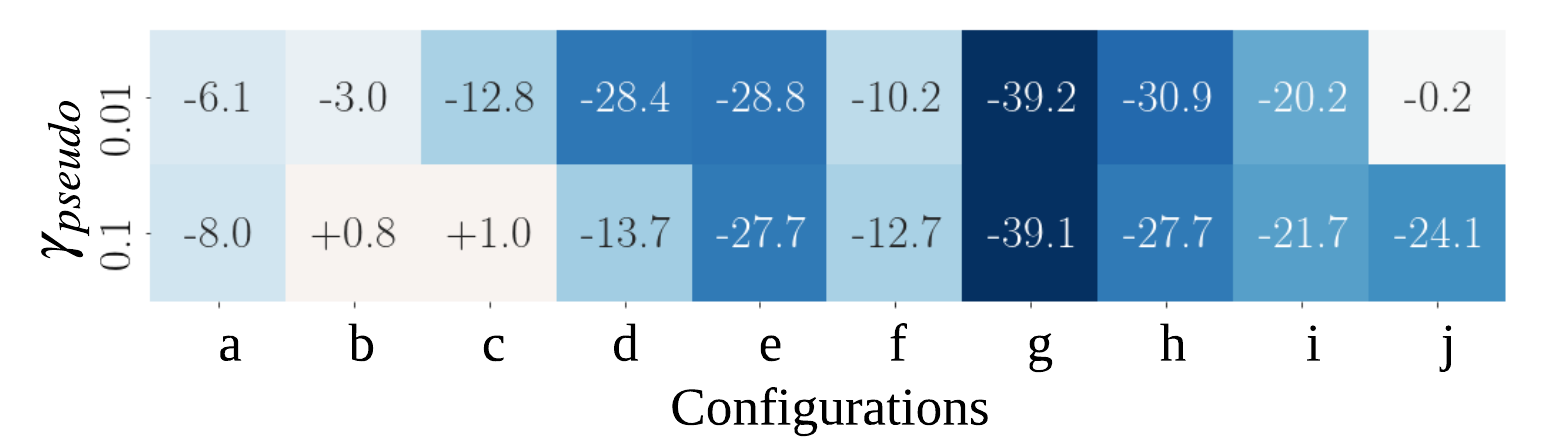
\includegraphics[width=\linewidth]{adkl/ablation/gamma-pseudo}
        \caption{\small Impact of the pseudo inputs trade-off parameter}
        \label{fig:gamma-pseudo}
    \end{subfigure}
    \hfill
    \begin{subfigure}[t]{0.26\textwidth}
        \centering
        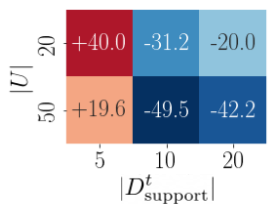
\includegraphics[width=\linewidth]{adkl/ablation/pseudo-gp}
        \caption{ $|U|$ in ADKL-GP}
        \label{fig:pseudo-gp}
    \end{subfigure}
    \caption{Relative decrease/increase in the meta-test MSE\\compared to no regularisation (lower is better)}
    \label{fig:ablation}
\end{figure}

First, \fig{gamma-task}, by comparing $\gamma_\mathrm{task} \in \LC 0.01, 0.1\RC $ relative to $\gamma_\mathrm{task} = 0$, \fig{gamma-task} demonstrates that regularizing the task encoder significantly improves the generalisation performance.
Other results presented in \append{ablation-taskreg} show that the conclusion holds for all support set sizes tested. It confirms the importance of using a task representation for generalisation in few-shot learning and the relevance of the regularisation term we introduced.

Then, \fig{gamma-pseudo} shows that improving the kernel map evaluations using \textit{pseudo-input representations} can significantly help the meta-generalisation performance of ADKL. The observation holds no matter the number of support examples (see \append{ablation-pseudo}), although the improvements were more consistent for smaller support sets: improving the kernel map estimations in these cases is more critical.

Finally, figures \ref{fig:pseudo-krr} and \ref{fig:pseudo-gp} illustrate how the number of pseudo-representations affects performance of ADKL-KRR and ADKL-GP differently.
In general, we can confirm that adding more pseudo-representations improves generalisation.
However, the improvements are more prominent with KRR in comparison to GP. It may be due to the fact that GP attributes a part of the modelling noise to the kernel evaluations, leading to more constraints on the optimisation of the pseudo-representation parameters.

We just went through the individual effect of the two hyper-parameters we introduced as part of the framework, see \append{ablation} for an analysis of their joint impact.


\subsubsection{Benchmarking analysis}

We compared ADKL to a number of other methods that are related to our work. We first compared the performance on the synthetic collection \texttt{Sinusoids}, and susbsequently on two real-world molecular collections, \texttt{Binding} and \texttt{Antibacterial}

\textbf{Conditional Neural Processes} (CNPs), proposed by \citet{garnelo2018conditional}, learn conditional stochastic processes parameterised by task-specific conditions derived from the support sets. By comparison, ADKL-GP also learns conditional stochastic processes but has mathematical guarantees thanks to gaussian processes and PSD kernels.

\textbf{Few-shot deep kernel learning} (R2D2) Proposed by \citet{bertinetto2018meta}, R2D2 is the meta-learning version of deep kernel learning seen in \sect{dkl-meta}. They tackle the lack of adaptation for new tasks by using Ridge regression, but do not adapt the kernel itself at test time.

\textbf{Learned Basis Function}, developed by \citet{Loo2019regression}, is linked to deep kernel learning since its output is a linear combination of the processed support examples. However, the architecture is trained to produce a task descriptor that is used to generate the weights for the final regressor directly. Hence, it adapts to the task, but does not explicitly train the task descriptor as ADKL does, and loses the principled approach of kernel regression by outputing weights directly.

% \textbf{Prototypical MAML} \citep{triantafillou2019meta} is a bridge between Prototypical Networks \citep{snell2017prototypical} and MAML that allows within-task adaptation by using MAML on top of a shared feature extractor.

\textbf{MAML} (see \sect{maml})

\textbf{Bayesian MAML} (BMAML): \citet{kim2018bayesian} proposed a Bayesian variant of MAML where a feature extractor is shared across tasks, while multiple MAML particles are used for the task-level adaptation.

These algorithms have all proven to have efficient and effective test-time adaptation routines and therefore constitute strong baselines for benchmarking.

For bioassay modelling benchmarks, we looked at the performance using solely ECFP4 (Extended Connectivity FingerPrints of diameter 4) as input representation. We made that decision to put every method on an equal footing and avoid letting the representation impact the performance. Moreover, we also compared ADKL to two single-task methods considered to be state-of-the-art in chemoinformatics \citep{olier2018meta}:
\begin{enumerate}[noitemsep, label=\alph*)]
  \item ECFP4 with random forest (ECFP4+RF)
  \item ECFP4 with kernel Ridge regression using tanimoto similarity as a kernel function (ECFP4+KRR)
\end{enumerate}

At test time, we computed the mean squared error (MSE) of every method on each task thirty times, using different support/query partitions (the partitions were the same for every method). This scheme mitigates the pobability that the result of a particular method on a task is obtained through blind luck, since the returned performance is averaged over thirty independent runs. In the following, I report the MSE averaged over every tasks.

\paragraph{Synthetic data}

\Tab{sinusoids} shows that ADKL achieves the best performance in every few-shot learning regime. I also provide a visualisation of the predictions from each model in \append{predictions}.

\begin{table}[ht]
  \centering
  \begin{tabular}{@{}lrrr@{}}
    \toprule
    $|\Dsupport|$ &     5  &     10 &     20 \\
    % model         &        &        &        \\
    \midrule
    BMAML         &  2.042 &  1.371 &  0.844 \\
    CNP           &  1.616 &  0.392 &  0.117 \\
    Learned Basis &  3.587 &  0.800 &  0.127 \\
    MAML          &  2.896 &  1.634 &  0.901 \\
    ADKL-GP    &  1.178 &  0.084 &  0.007 \\
    ADKL-KRR   &  \textbf{0.867} &  \textbf{0.061} &  \textbf{0.005} \\
    % ProtoMAML     &  2.044 &  1.369 &  0.846 \\
    R2D2          &  1.002 &  0.073 &  0.009 \\
    \bottomrule
  \end{tabular}
  \caption{Average MSE on \texttt{Sinusoids}}
  \label{tab:sinusoids}
\end{table}

We note that the kernel methods perform much better in this scenario. One interpretation is that using kernels, ADKL and R2D2 are able to construct an embedding where sine functions are favoured. By contrast, initialisation-based methods such as MAML need an extremely expressive model to produce an initialisation that can properly adapt to sine waves of different characteristics.


\paragraph{Real-world bioassays}

Tables \ref{tab:results-antibacterial} and \ref{tab:results-binding} present the results on the  \texttt{Antibacterial} and \texttt{Binding} collections, respectively.

\begin{table}[ht]
  \centering
  \begin{tabular}{@{}lrrr@{}}
    \toprule
    $|\Dsupport|$ &               5  &               10 &               20 \\
    % model        &                  &                  &                  \\
    \midrule
    ADKL-KRR     &  0.0380 $\pm$ 0.0020 &  0.0348 $\pm$ 0.0009 &  0.0322 $\pm$ 0.0020 \\
    BMAML        &  0.0813 $\pm$ 0.0571 &  0.0486 $\pm$ 0.0071 &  0.0487 $\pm$ 0.0012 \\
    CNP          &  0.0416 $\pm$ 0.0019 &  0.0393 $\pm$ 0.0030 &  0.0397 $\pm$ 0.0027 \\
    ECFP4+KRR    &  0.0376 $\pm$ 0.0012 &  0.0352 $\pm$ 0.0014 &  0.0317 $\pm$ 0.0016 \\
    ECFP4+RF     &  \textbf{0.0373 $\pm$ 0.0012} &  \textbf{0.0339 $\pm$ 0.0013} &  \textbf{0.0311 $\pm$ 0.0012} \\
    % ECFP4+RF     &  \textbf{0.0373 $\pm$ 0.001} &  \textbf{0.0339 $\pm$ 0.001} &  \textbf{0.0311 $\pm$ 0.001} \\
    LearnedBasis &  0.0761 $\pm$ 0.0040 &  0.0754 $\pm$ 0.0042 &  0.0616 $\pm$ 0.0215 \\
    R2D2         &  0.0492 $\pm$ 0.0015 &  0.0460 $\pm$ 0.0110 &  0.0342 $\pm$ 0.0012 \\
    \bottomrule
  \end{tabular}
  \caption{Average MSE on \texttt{Binding}}
  \label{tab:results-binding}
\end{table}

\Tab{results-binding} shows a sad truth about computational drug discovery: datasets are so noisy and and ill-prepared that in some cases, learning across task can have no effect on the results. In this case, the best estimator of molecular binding is the single-task algorithm random forest using ECFP4 fingerprints. However, we do note that ADKL is a close second, performing significantly better than other methods.

\begin{table}[ht]
  \centering
  \begin{tabular}{@{}lrrr@{}}
    \toprule
    $|\Dsupport|$ &               5  &               10 &               20 \\
    % model        &                  &                  &                  \\
    \midrule
    ADKL-GP      &  0.1017 $\pm$ 0.0013 &  0.0895 $\pm$ 0.0015 &  \textbf{0.0860 $\pm$ 0.0016} \\
    ADKL-KRR     &  \textbf{0.1000 $\pm$ 0.0012} &  \textbf{0.0893 $\pm$ 0.0015} &  0.0862 $\pm$ 0.0009 \\
    BMAML        &  0.1059 $\pm$ 0.0021 &  0.1020 $\pm$ 0.0029 &  0.4616 $\pm$ 0.4210 \\
    CNP          &  0.1063 $\pm$ 0.0023 &  0.1239 $\pm$ 0.0219 &  0.1382 $\pm$ 0.0049 \\
    ECFP4+KRR    &  0.1166 $\pm$ 0.0020 &  0.1003 $\pm$ 0.0009 &  0.0956 $\pm$ 0.0009 \\
    ECFP4+RF     &  0.1129 $\pm$ 0.0002 &  0.1016 $\pm$ 0.0008 &  0.0970 $\pm$ 0.0003 \\
    LearnedBasis &  0.1274 $\pm$ 0.0037 &  0.1308 $\pm$ 0.0032 &  0.1329 $\pm$ 0.0043 \\
    R2D2         &  0.1104 $\pm$ 0.0023 &  0.0962 $\pm$ 0.0021 &  0.0921 $\pm$ 0.0010 \\
    \bottomrule
  \end{tabular}
  \caption{Average MSE on \texttt{Antibacterial}}
  \label{tab:results-antibacterial}
\end{table}

On the other hand, \tab{results-antibacterial} confirms that in some cases, using meta-learning can indeed help. When and why meta-learning can perform better is an open question and very much an active field of research. In the meantime, computer biochemists need to test both approach before they can settle for one, provided they have enough data to spare on a validation study...



\subsubsection{Active learning}

Active learning is a paradigm where the trained algorithm is provided both labelled and unlabelled examples. It can interact with the teacher to query new labels as learning progresses, such that queried samples can maximise the information gathered about the task.
This setting is particularly relevant in a biochemistry context, where labelling is slow and costly: using active learning, experimenters can choose to prioritise molecules that will incur more information for the trained algorithm. With a well-tuned active-learning algorithm, biochemists could make \textit{in vitro} testing on a handful of molecules, and then explore the rest of the molecular space using the queries from the model.

For an algorithm to be useable in an active learning setting, it needs to be well-calibrated. To wit, it should be able to assess its level of confidence on the predictions is produces. ADKL, when used with a gaussian process estimator, provides a predictive variance and can therefore be used for active learning. Hence, we tested ADKL-GP in this setting on our three collections. We compared the results with those of CNP, since it also output a predictive distribution.

During the experiment, training was performed using support sets of five examples. At test-time, we randomly partition each task from the meta-test set into three subsets:
\begin{enumerate}[itemsep=1pt,label=\alph*)]
  \item A support set $\Dsupport$, containing only five examples;
  \item A query set $\Dquery$, to compute the generalisation error;
  \item A pool of unlabelled data $D_\mathrm{u}$.
\end{enumerate}

First, the algorithm adapts to the task using $\Dsupport$ to constitute the initial hypothesis. Then, it updates iteratively by querying the most informative sample from $D_\mathrm{u}$, in our case using a maximum entropy criterion. The iterative adaptation continues until the allocated budget runs out or the unlabelled pool is entirely consumed. These steps are presented more formally in \algo{active}.

\begin{algorithm}[ht]
  \caption{Active learning on a new task $t$}
  \label{algo:active}
  \begin{algorithmic}[1]
    \REQUIRE learning algorithm with a probabilistic output
    \REQUIRE $l$: labelling function
    \REQUIRE $\Dsupport$, $\Dquery$ and $D_\mathrm{u}$: support, query and unlabelled sets
    \REQUIRE $b$: the query budget
    \STATE Adapt algorithm to the task using $\Dsupport$
    \WHILE{$b > 0$ or $D_\mathrm{u}$ not consumed}
      \STATE Select maximum entropy sample $\vx^* = \argmax_{\vx \in U}{\E \LB \log p(y \mid \vx, \Dsupport) \RB}$
      \STATE Update $\Dsupport \gets \Dsupport \cup \{\vx^*, l(\vx^*)\}$
      \STATE Update $D_\mathrm{u} \gets D_\mathrm{u} \{\vx^*\}$ and $b \gets b-1$
      \STATE Re-adapt algorithm using the updated support set.
    \ENDWHILE
  \end{algorithmic}
\end{algorithm}

In the following, we report the results obtained for query budgets up to $b = 20$. In the case of the \texttt{Sinusoidal} collection, we could spare repeating the experiments a number of times in order to obtain a standard deviation. However, it was too time-consuming and costly to do so on \texttt{Binding} or \texttt{Antibacterial}, given the complexity of the networks for this task.

\begin{figure}[ht]
  \makebox[\linewidth][c]{
    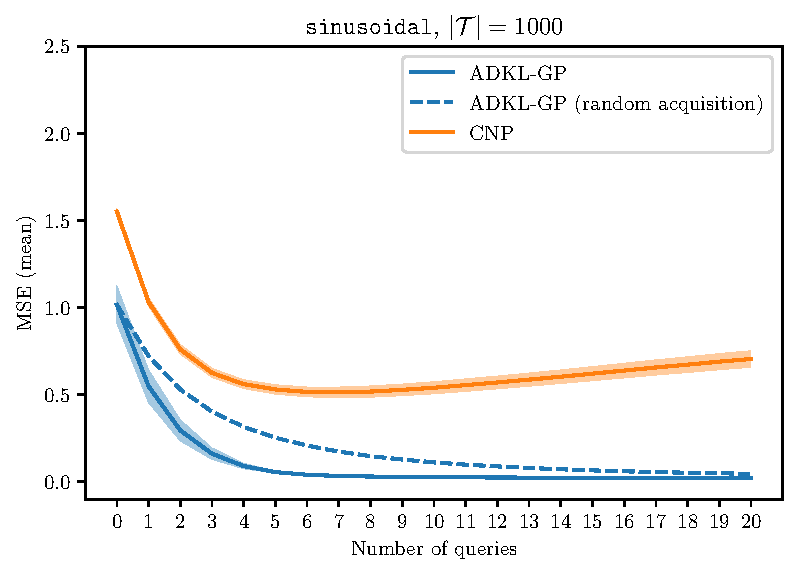
\includegraphics[height=6cm]{adkl/active/T1000-K5-msemean}
    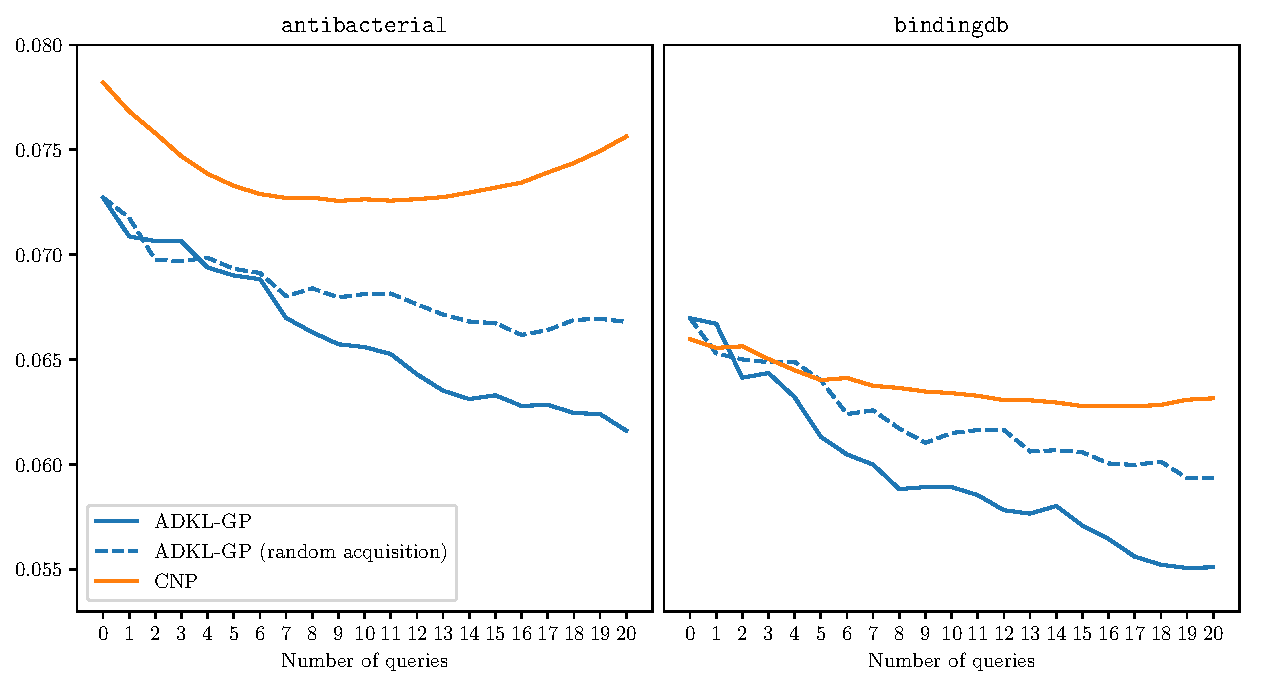
\includegraphics[height=6cm]{adkl/active/real-world}
  }
  \caption{Average MSE performance with active learning\\for query budgets up to $b = 20$}
  \label{fig:active}
\end{figure}

\Fig{active} illustrates that under the active learning strategy, ADKL-GP consistently outperforms CNP.
In particular, we observe that very few samples are queried by ADKL-GP to capture the data distribution whereas CNP performance quickly plateaus.

Moreover, since using the maximum predictive entropy strategy is better than querying samples at random (solid vs. dashed line), these results suggest that the predictive uncertainty provided by ADKL-GP is informative and the algorithm is relatively well calibrated.

When the number of queries is greater than $10$, we observe a performance degradation for CNP while ADKL-GP remains consistent.
This observation highlights the generalisation capacity of deep kernel learning methods, even outside the few-shot regime where they have been trained ---a property that does not hold true for CNP.


% \subsection{Conclusion}

In conclusion, the adaptive deep kernel learning framework is a simple yet powerful novel method that is able to accumulate knowledge across a number of related tasks, and leverage this knowledge at test-time to outperform other methods on synthetic testbeds but also –and more importantly for InVivo AI– when it comes to evaluating biochemical properties in a few-shot learning setting. What is more, ADKL is well-calibrated, making it a well-suited framework for computational biochemistry since it cannot only predict the correct output from a very narrow set of examples but also guide the costly exploration of the chemical space to optimize the information obtained from \textit{in vitro} testing.



% \clearpage
% \section{Other endeavours}
%
% Although working on ADKL was by far my main centre of attention during the internship, it was not the sole focus. Indeed, we raised fascinating research questions over the last eight months, and I would like to introduce some of them to you.
%
% % Note however that these subjects are largely on-going research at InVivo AI, so I do not have results to advertise.
%
% \subsection{Synthetic molecular data}
%
% The major obstacle that hinders computational drug discovery resides in the dire lack of clean and abundant data to train on. Without
%
%
% \subsection{Understanding meta-learning}
%
% Most of my work at InVivo AI revolved around meta-learning. Applying the field to a domain as difficult as drug discovery, it quickly became apparent that much remains to be explored within the discipline. For one thing, it is unclear how the distribution of tasks influences learning.
% Defining a task distribution is in itself perplexing. In some simple cases, like the synthetic \texttt{Sinusoids} collection, we can naturally work on the distribution parameters. But transpose the issue to any real-world problem and it becomes problematic.
%
% Towards the end of the internship, we started a project with Tristan Deleu from Mila to assess the impact of the task distribution on the performance. We wanted to see if modifying the sampling method would help curb issues such as negative adaptation \citep{deleu2018effects}.
%
% Moreover, one of our goal was to see how different algorithms would cope with a multi-modal task distribution. We expected uni-modal methods such as MAML to perform poorly on such task distribution whereas methods such as BMAML or ADKL, equipped to deal with more diverse tasks, would be better of.
%
% Unfortunately, the internship ended before I could see the end of the project.
%
%
% \subsection{A better representation}
%
% The crux of machine-learning for drug discovery resides in obtaining a meaningful representation of molecules. In our work on ADKL, we ignored the issue for the duration of the paper to focus on the method itself, using ECFP4 representation directly. However, it is clear that we lack a representation informative enough to use the full potential of learning algorithms on drug discovery.
%
% The last project I participated to, although briefly, dealt with this very issue. We began with a simple observation: there are a myriad of ways to represent a molecule. I have discussed a few machine-learning-ready methods in \sect{representation}, but there many more. For example, you can represent a molecule using its standardised \href{https://en.wikipedia.org/wiki/IUPAC_nomenclature_of_organic_chemistry}{IUPAC name}, its graph representation or even an image of its 2D configuration.
%
% To produce a better molecular representation, we wanted to leverage this plurality of representations using a contrastive coding method, such as the contrastive multiview coding developed by \citet{tian2019contrastive}. The idea behind contrastive multiview coding is to use all representations available, and train an unsupervised model to learn a coherent latent space model wherein different views of the same object will be close to each other.
%
% Using this method, which to the best of our knowledge has not been tried before in a drug discovery context, we can even exploit scientific publications and lab reports discussing the compound, widening tremendously the horizon of what can be included to train the representation.
%
% I left InVivo AI at an early stage of the project, but it is continued by the rest of the team, helped with collaborators from Mila and McGill University.
%
%
% % \subsection{Training to extrapolate}
% %
% % As I have mentionned, computational biochemists work under the implicit assumption of compositionality, which lets us hope to be able to extrapolate extracted knowledge from one part of the molecular space to another. I do not expect extrapolation alone to give us the full story. However, it might be good enough to scout the vast molecular space in a much more efficient way than what is currently considered the state-of-the-art (namely blind luck, a harsh observer would say).
% %
% % The question remains: how can we teach our algorithms to extrapolate?



\clearpage
\section*{Conclusion}
\addcontentsline{toc}{section}{Conclusion}

% InVivo AI strives to push the boudaries of computational drug discovery ever further, through intense efforts in both applied and fundamental research. In this report, I aimed to present the projects on which I worked as a research intern there during the last eight months of last year.

Computational drug discovey is challenging. The subject matter itself is extremely complex: molecules form elaborate structures whose basic properties, let alone their effect on human health, are inherently tricky to predict and would necessitate extremely expressive machine-learning algorithms, complex enough to extract deeply nested information. Such algorithm would need clean and abundant data so they can be trained, but the sad truth about drug discovery is that in this field, data is neither plentiful nor orderly.

However, datasets do come in numbers: we may not have large sets of examples related to one given task, but we do have a few datapoints for a huge number of bioassays. Hence, we can hope to tackle computational drug discovery through two ways: we can either start producing clean and abundant data, requiring massive investments, or we may work to capture information from every source at our disposal.

At InVivo AI, we have chosen the second route and strive to push the boudaries of computational drug discovery ever further, through intense efforts in both applied and fundamental research. As an intern there, I worked on the bleeding edge of research in meta-learning, a paradigm that seeks to learn how to learn from multiple tasks at once. I took part in developing ADKL (adaptive deep kernel learning), a novel framework that explicitly adapts to new tasks at test time. The method is a step in the right direction and a good candidate to lead the advent of computational drug discovery, but it is certainly not the final answer.

There is still much to understand about meta-learning. From the influence of the task distribution to the causes of negative adaptation, the inner workings of learning to learn remain largely a mystery. During my internship, I tried to bring some answers to these fundamental questions.

Through this report, I wanted to introduce the reader to the world of computational biochemistry, since I expect they will mostly be coming from the same background as I did, namely mathematics and computer science. I pointed at on-going research in the field of meta-learning that tackle the same kind of issues that drug discovery faces, and I presented the research I did working on ADKL.



% Meta-learning is not the panacea. First, there is still much to understand about the field, and we launched research projects in that direction
% Computational drug discovery also needs an array of techniques ranging from generation and exploration algorithms to better molecular representation before we can hope to perform direct compound optimisation to produce new treatments. Moreover,

% In this report, I aimed to present the projects on which I worked as a research intern there during the last eight months of last .
%
%
% Hence, we need p
%
% Because InVivo AI works in the field of drug discovery, I wanted to start this report with a gentle introduction on computational biochemistry. Far from being a pundit myself, I am optimistic to have gathered enough information on the field to be able to do so, and I hope it can work as a review of the bare essentials for future recruits at InVivo AI who, like I did, come from a computer science rather the chemistry background.
%
% Over the course of the internship, my main focus was on fundamental research in meta-learning, the avenue we have chosen to explore at InVivo AI to tackle the challenges posed by computational drug discovery. Hence, I presented the articles I
%
%
%
% My internship at InVivo AI has allowed me a glimpse at fundamental research in the field of computational biochemistry.



\clearpage
\section*{Acknowledgement}
\addcontentsline{toc}{section}{Acknowledgement}

I would like to express my deepest gratitude to my supervisor, Prudencio Tossou, for his patient guidance, enthusiastic encouragements and useful critiques. He provided me with precious advice, corrected my code and nudged me in the right direction every time I needed it.

In fact, I wish to thank the entire team at InVivo AI, who made this internship a formidable experience personally as much as professionally. Their continued technical and emotional support got me through the hard times rushing for a deadline or waiting for a review. I am particularly thankful for the many ping-pong and coffee breaks that kept my sanity in checks in these times of turmoil.
My experience of this internship would have been very different had it not been for them.

My internship was also made a wonderful experience by my friends and collegues, from Mila and elsewhere. Julien, Paul, Mandana, Clément and Tristan, in particular, helped me a great deal over the last eight months, giving me perspective, letting me think out loud and providing me with numerous insights that unlocked me more than once.

I would also like to address special thanks to Cem Subakan and Aurélie Hélouis from Mila. Cem gave me guidance during the internship, offering his research acumen and standing for the numerous changes in the project we were working on together. Aurélie helped me a great deal throughout my Master's at Mila, and especially over the course of my internship.

Last but not least, I want extend my thanks to the people of the Mitacs Acceleration Program who deserve praise for making the internship a possibility. They have worked hard to provide diligent assistance and funding, and I am extremely grateful to them.

% \nocite{*}
\bibliography{bibliography,references}
\bibliographystyle{abbrvnat}

\appendix

\section{Few-shot regression collections}
\label{app:collections}

There is a dire need in the meta-learning community for standardised benchmarks, especially in the case of few-shot regression. To wit, meta-learning research is dominated by image classification, owing in part to the fact that such problems validate the assumptions of the field quite well -- learning to recognise shapes can indeed be learned accross a variety of classification tasks.

Thus, in the case of image classification, benchmarks exist. For instance, \citeauthor{triantafillou2019metadataset} from Google Research have proposed in \citeyear{triantafillou2019metadataset} ``Meta-Dataset'', a collection of image classification datasets to be used as a testbed by the community.

On the contrary, the few-shot regression community mostly relies on \textit{ad hoc} meta-datasets, with little systematic benchmarking other than on synthetic data. I for one believe that synthetic testing is most important in fundamental research, since it helps pinpoint the capabilities of an algorithm by controlling explicitly the assumptions one can make on the data. However, we do need to challenge ourselves to real-world applications, lest meta-learning remain a niche and unapplicable discipline.

In what follows, I describe four meta-datasets we work with at InVivo AI.

\subsection{A synthetic meta-dataset : the \texttt{Sinusoids} collection}
\label{app:collections-synthetic}

This synthetic few-shot regression benchmark, introduced by \citet{kim2018bayesian}, consists of 5,000 tasks defined by functions of the form :
\begin{align}
  y &= A \sin(\omega x + b) + \varepsilon &
  &\text{with}&
  &
  \begin{matrix}
    A \in \LB 0.1, 5.0 \RB \\
    b \in \LB 0.0, 2\pi \RB \\
    w \in \LB 0.5, 2.0 \RB \\
    \varepsilon \sim \normal \LP 0,(0.01 A)^2 \RP
  \end{matrix}&
\end{align}

The examples are generated by sampling inputs $x$ from the $[-5.0, 5.0]$ interval, as well as the observation noise $\varepsilon$. The tasks themselves are divided into a meta-train, a meta-validation and a meta-test sets, which contain respectively 56.25\%, 18.75\% and 25\% of the functions.

By design, this synthetic collection validates the assumptions of meta-learning : the functions are indeed sampled from a task distribution, and the goal of the algorithm is to learn to recognise the parameters of the sine function from very few points.

The \texttt{Sinusoids} collection, although it may be given other names, has become a standard benchmarking tool in the community.



\subsection{\texttt{Binding} and \texttt{Antibacterial}, two real-world collections}
\label{app:collections-real}

One important flaw in the \texttt{Sinusoids} collection is its lack of realism. Moreover as a drug discrovery company, InVivo AI strive to develop algorithms that work on real-world, bio-chemical data.

To that end we propose two collections, whose content is \href{https://github.com/invivoai/molecular-datasets}{available here}, compiled from data in the public domain. Both contain data from bioassays that are representative of real-world few-shot regression tasks that arise in drug discovery.

\begin{figure}[ht]
  \makebox[\linewidth][c]{
    \begin{subfigure}[t]{.5\textwidth}
      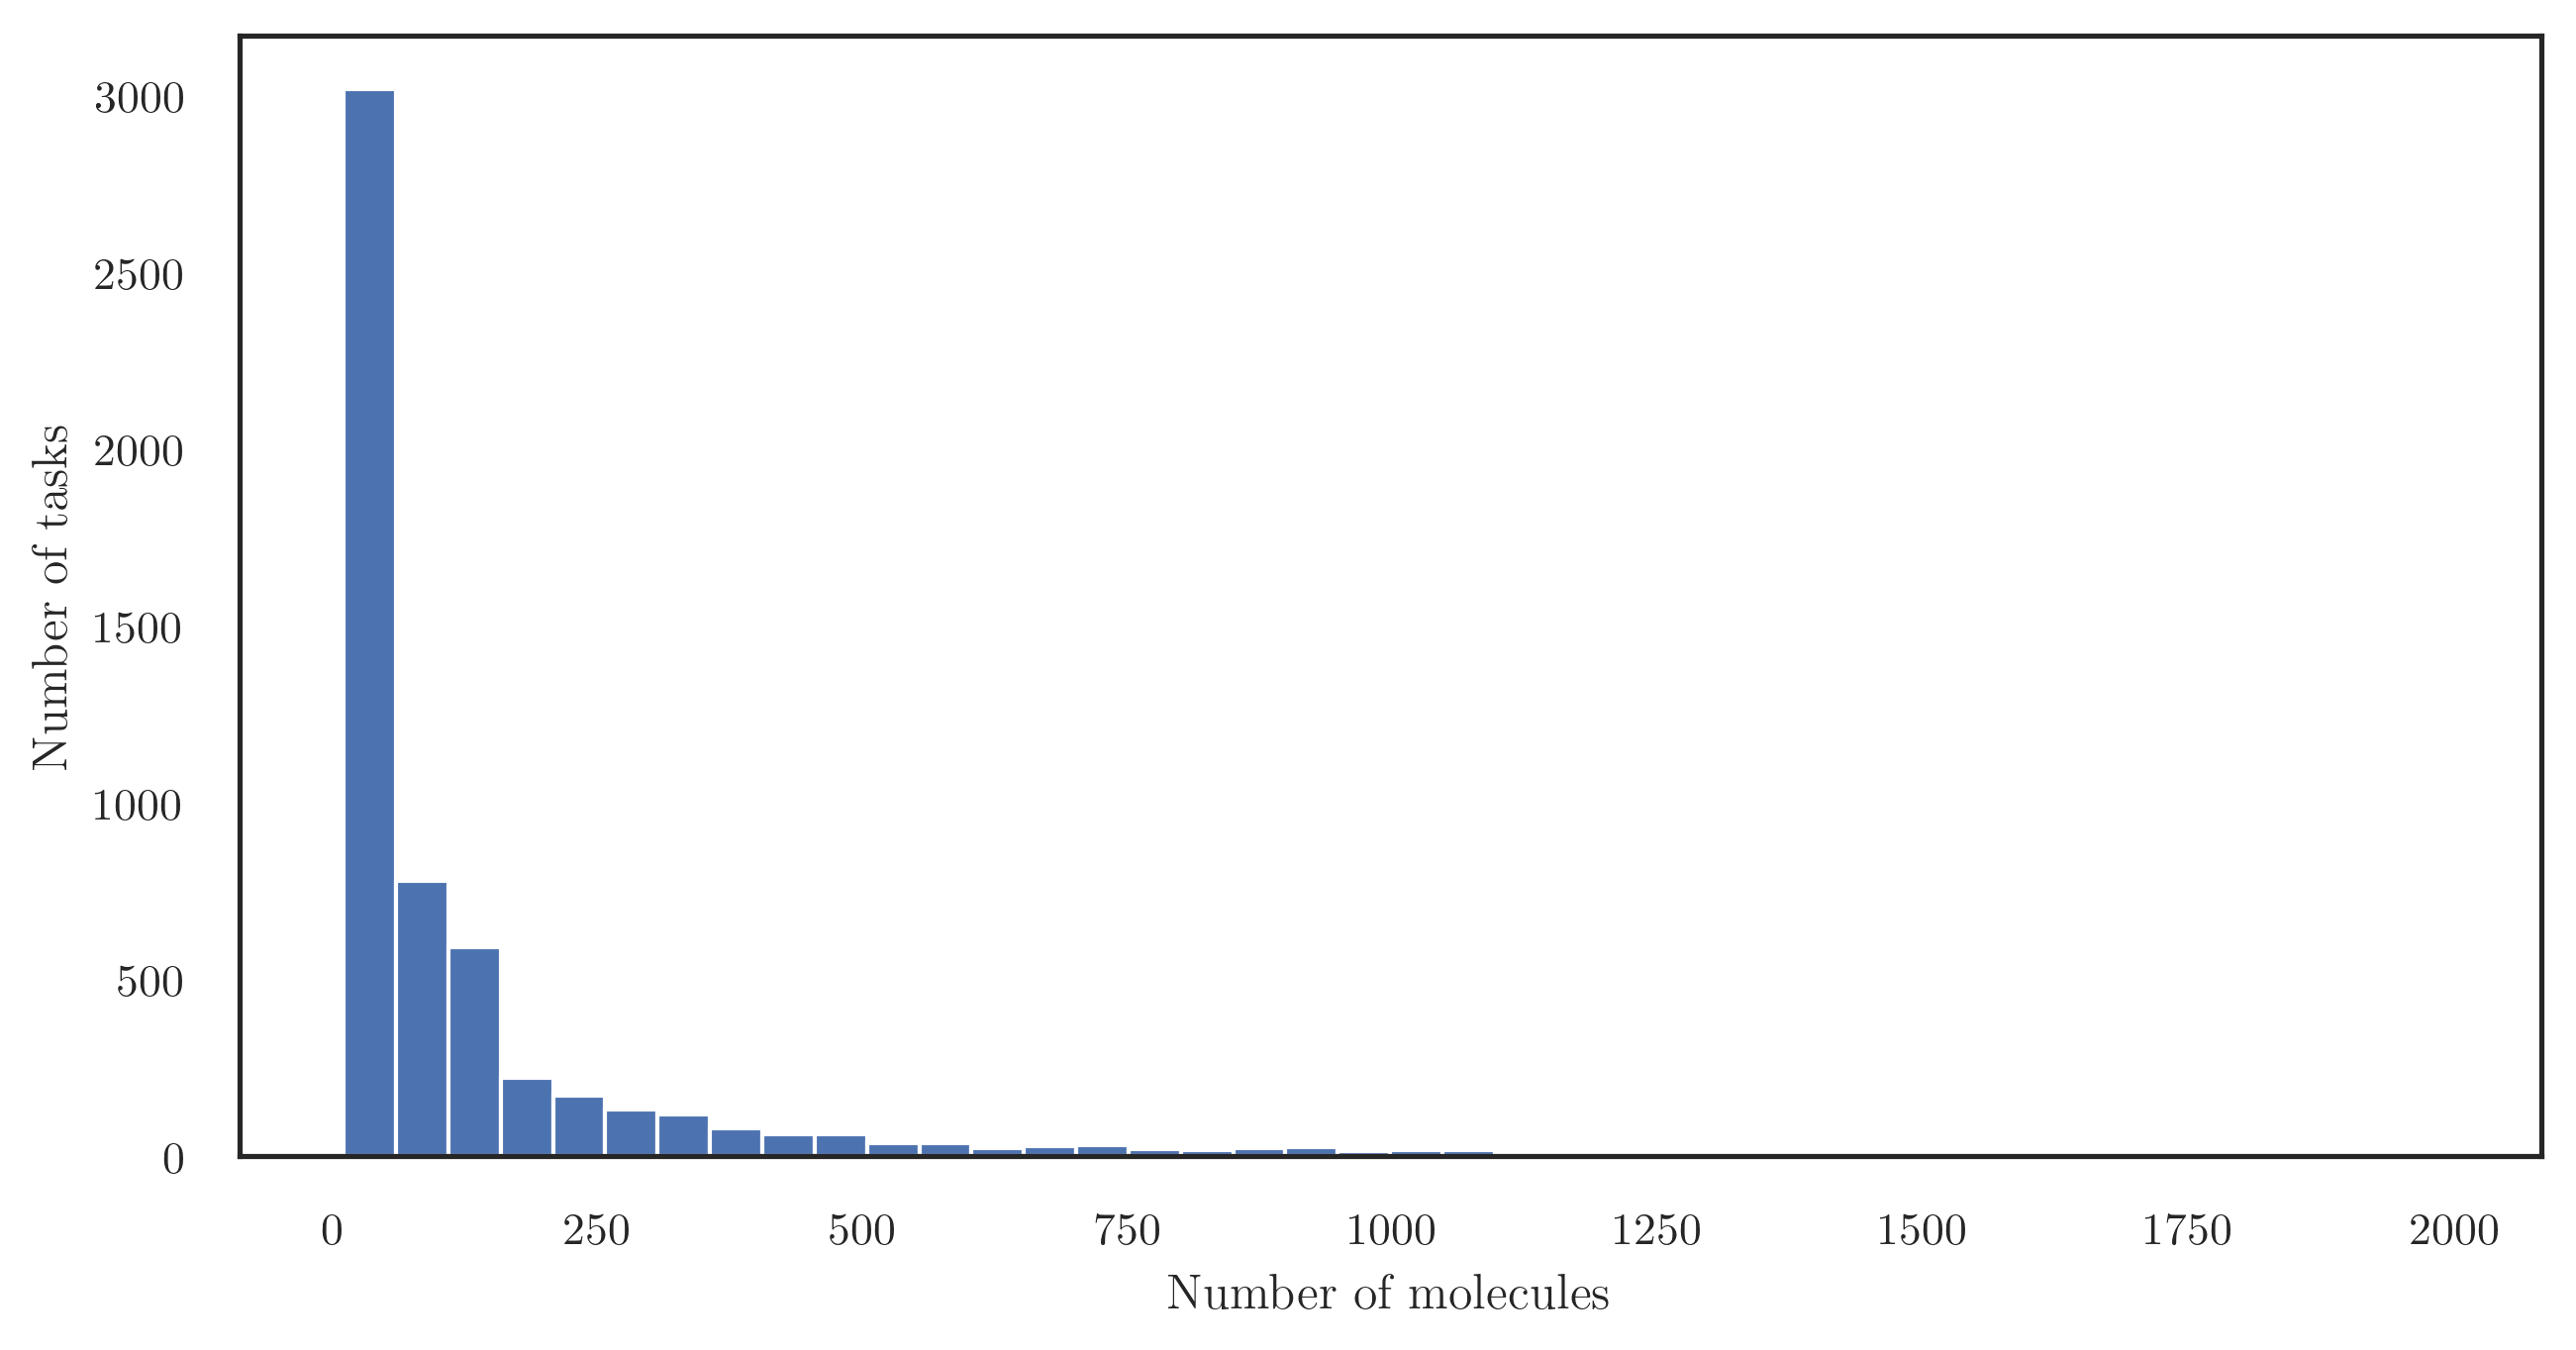
\includegraphics[width=1\textwidth,center]{datasets/hist-binding}
      \caption{\texttt{Binding}}
      \label{fig:hist-binding}
    \end{subfigure}
    \hspace{1cm}
    \begin{subfigure}[t]{.5\textwidth}
      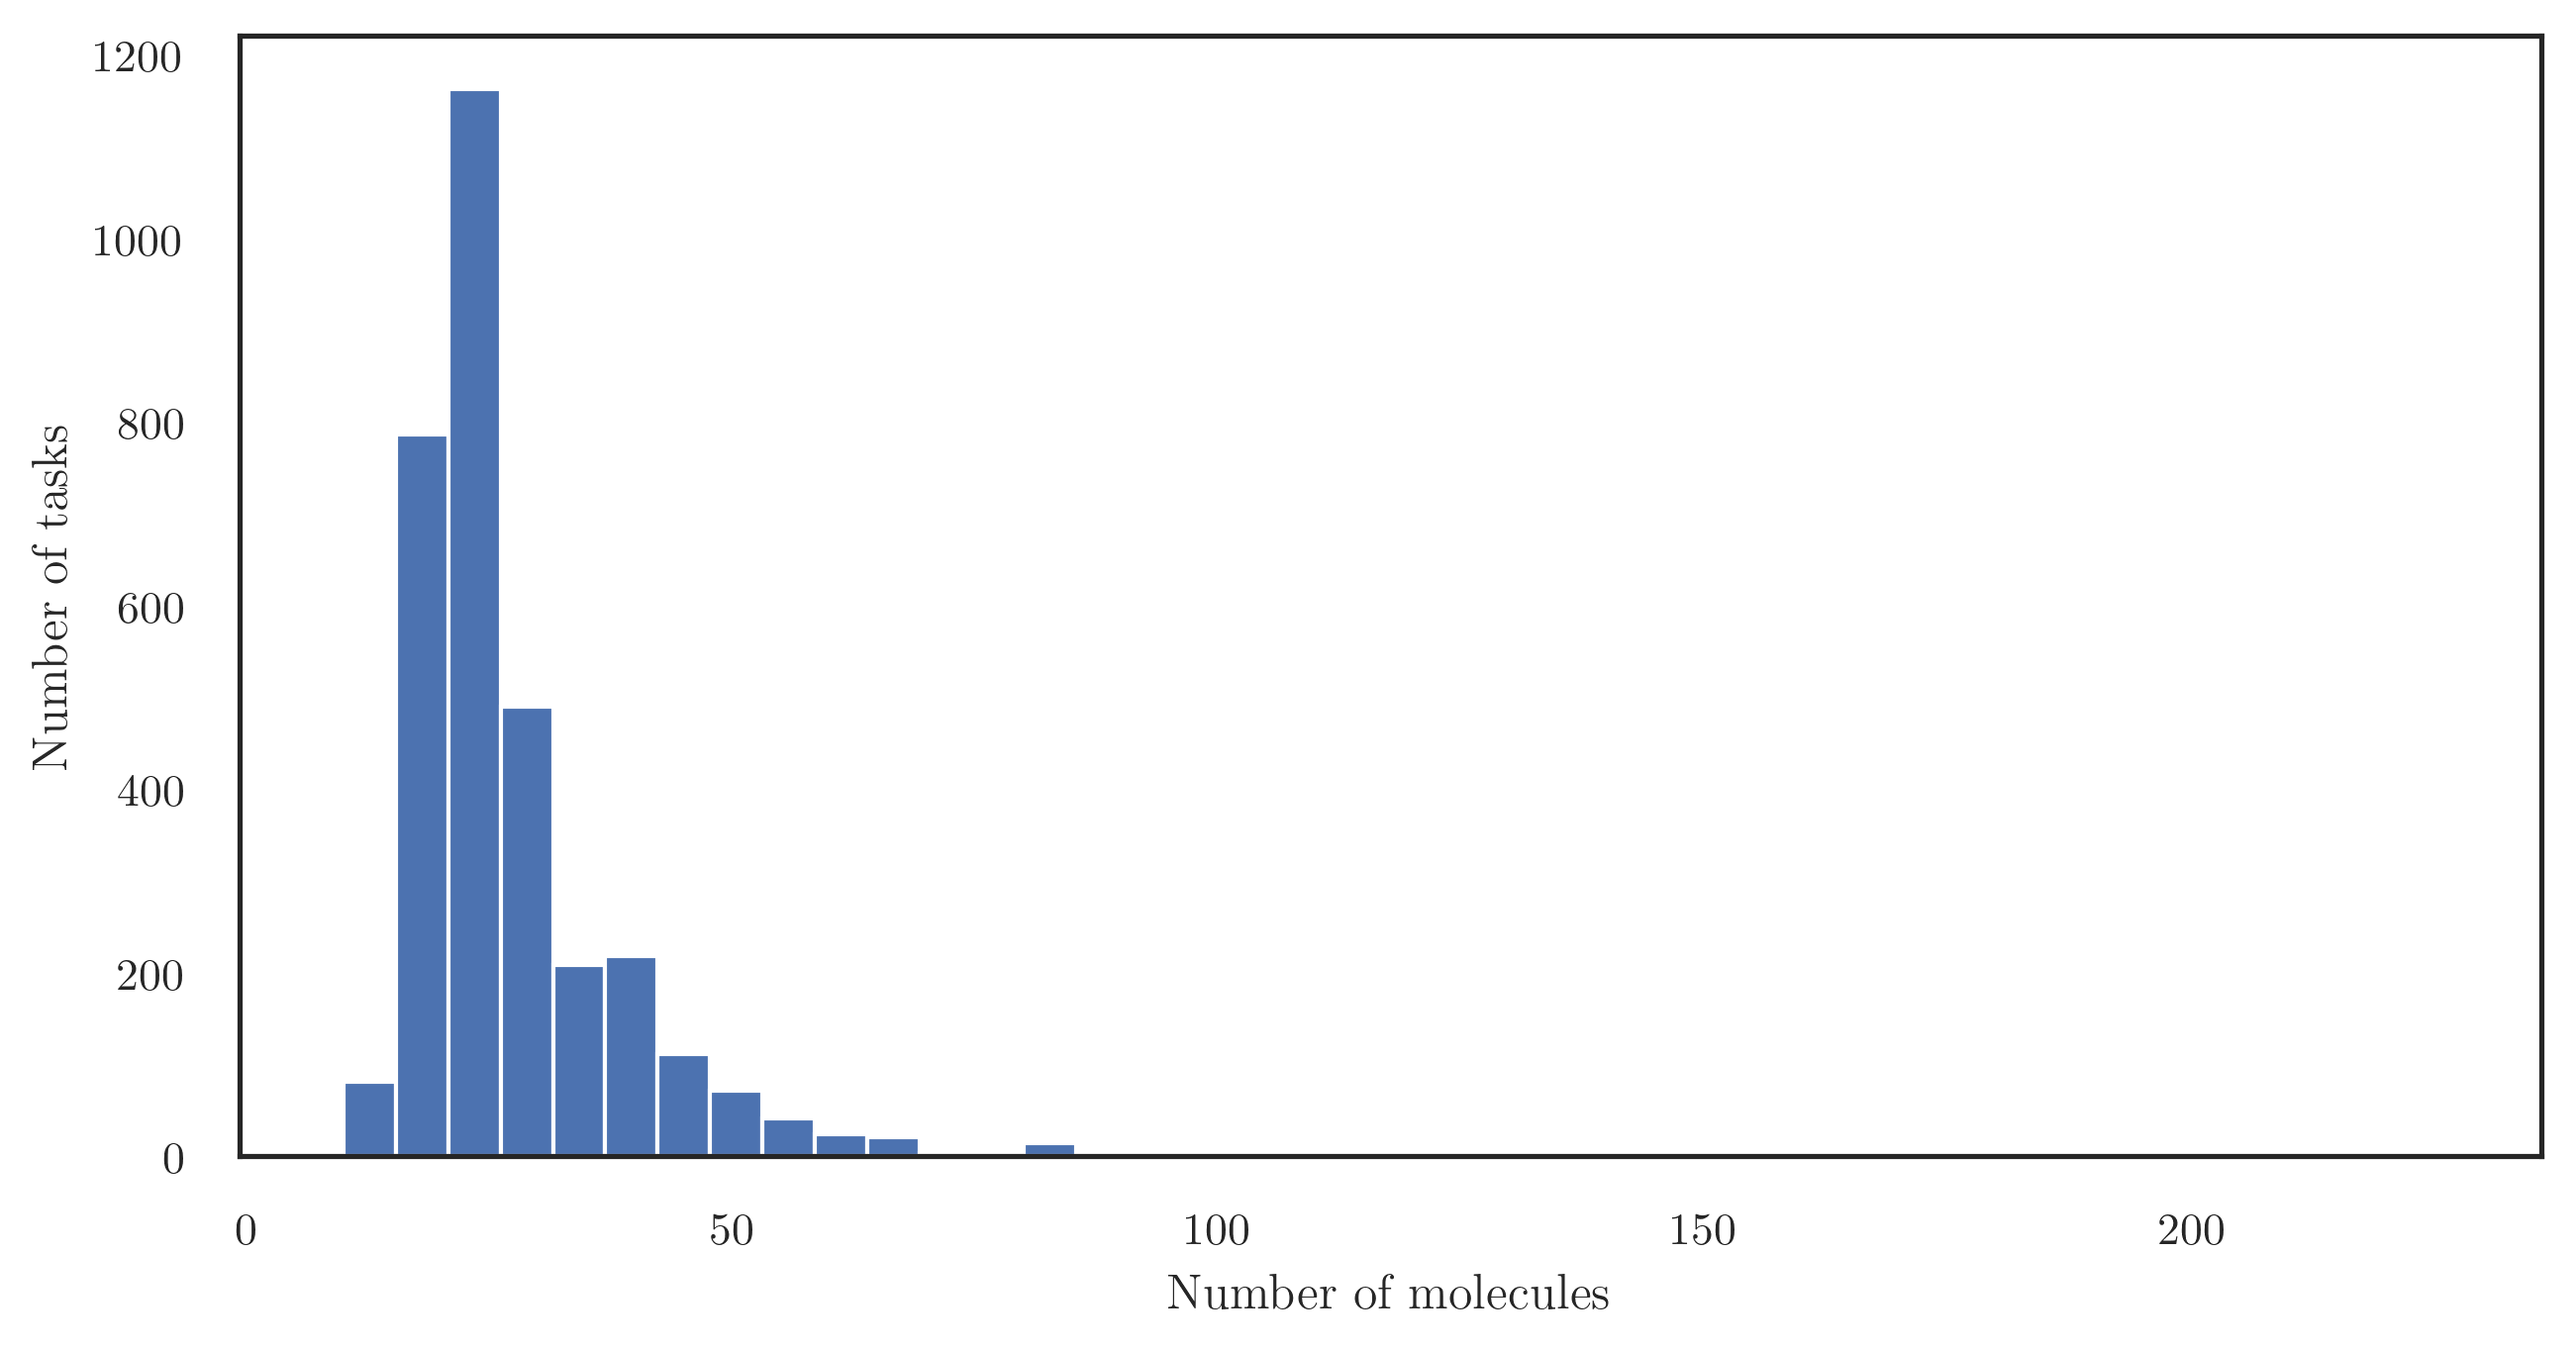
\includegraphics[width=1\textwidth,center]{datasets/hist-antibacterial}
      \caption{\texttt{Antibacterial}}
      \label{fig:hist-antibacterial}
    \end{subfigure}
  }
  \caption{Distribution of the number of examples in each task\\for the \texttt{Binding} and \texttt{Antibacterial} collections}
  \label{fig:histograms}
\end{figure}

\Fig{hist-binding} shows just how scarce data is for both collections, reflecting the time and money needed to perform an exhaustive mapping of the molecular space using \textit{in vitro} and \textit{in vivo} testing.

\subsubsection{\texttt{Binding}}
\label{app:collections-binding}

This collection is extracted from the public database \href{www.bindingdb.org}{BindingDB} \citep{liu2007bindingdb}. We altered it by removing bio-assays with targets correlated above $0.8$ or those with less than 10 experimental measurements, leaving 5,717 tasks.

Each task from the collection reports the binding affinity of small molecules to a target protein. Hence, the task distribution is defined by the characteristics of the proteins.

\subsubsection{\texttt{Antibacterial}}
\label{app:collections-antibacterial}

This task collection is extracted from \href{https://pubchem.ncbi.nlm.nih.gov/}{PubChem} \citep{kim2019pubchem}, a public registery of molecules and bioassays. After also removing bio-assays with correlations above $0.8$ and those with less than 10 samples, we obtain $3,255$ tasks.

Each task in \texttt{Antibacterial} reports the antibacterial effect of a set of small molecules on a given strain of bacterium. More specifically, it describes the minimum concentration needed to wipe out at least half the population of bacteria.

Note that this collection is particularly noisy. Indeed, the results are obtained by testing different concentrations of the same molecules, leading to discrete approximation riddled with thresholding effects.


\subsection{A synthetic collection of molecular data : \texttt{Properties}}
\label{app:collections-properties}

The noise issue in the two bioassay collections led us at InVivo AI to create another meta-dataset, which we called \texttt{Properties}.

Although \texttt{Properties} is a collection of synthetic tasks, it still relates to drug discovery. Hence, is reports a set of 767 computable physico-chemical properties for more than 600,000 molecules, thus completely removing the noise issue while providing a rich benchmarking tool to computational bio-chemists.

With properties, the community can test out algorithms specifically designed for molecular scoring with the challenges it entails (such as the representation issue), while still benefiting from a very large dataset.



\clearpage
\section{Ablation study}
\label{app:ablation}

This section presents more results from the ablation study. See the \href{https://openreview.net/pdf?id=Syeu8CNYvS}{ICLR submission} for a more comprehensive presentation.

\subsection{Task regularisation}
\label{app:ablation-taskreg}

\Tab{app-ablation-tasks} presents the hyper-parameter combinations used in the experiments to assess the impact of the trade-off parameter $\gamma_\mathrm{task}$.
We report the MSE performance obtained on the meta-test for each configuration.

\begin{table}[ht]
  \centering
  \makebox[\linewidth][c]{
  \begin{tabular}{@{}lllllrrr@{}}
    \toprule
                &    &                  &      & $\gamma_\mathrm{task}$ &    0.00 &    0.01 &    0.10 \\
    Conf. & algorithm & K & architecture & $\gamma_\mathrm{pseudo}$ &         &         &         \\
    \midrule
    a & ADKL-KRR & 20 & attention & 0.01 &  0.0585 &  0.0327 &  \textbf{0.0289} \\
    b &             & 10 & deepset & 0.00 &  0.4051 &  \textbf{0.2944} &  0.3671 \\
    c &             &    &                  & 0.10 &  0.4363 &  0.2964 &  \textbf{0.2882} \\
    d & ADKL-GP & 5  & attention & 0.10 &  2.4920 &  \textbf{2.2511} &  2.2994 \\
    e & ADKL-KRR & 20 & attention & 0.00 &  0.0574 &  0.0305 &  \textbf{0.0302} \\
    f & ADKL-GP & 5  & attention & 0.01 &  2.5611 &  \textbf{2.1511} &  2.2112 \\
    g &             &    & deepset & 0.01 &  3.2933 &  \textbf{2.7663} &  3.0971 \\
    h &             & 10 & deepset & 0.01 &  0.7675 &  0.7105 &  \textbf{0.4352} \\
    i &             & 20 & deepset & 0.00 &  0.1201 &  0.0873 &  \textbf{0.0646} \\
    j & ADKL-KRR & 20 & attention & 0.10  & 0.0575 &  0.0447 &  \textbf{0.0273} \\
    \bottomrule
  \end{tabular}}
  \caption{Effect of using task regularisation (parameter $\gamma_\mathrm{task}$) on the MSE performance}
  \label{tab:app-ablation-tasks}
\end{table}

To make reading this table easier, we also repeat \fig{gamma-task} showing the improvement of the MSE relative to $\gamma_\mathrm{task} = 0$ (no regularisation).

\begin{figure}[ht]
  \centering
  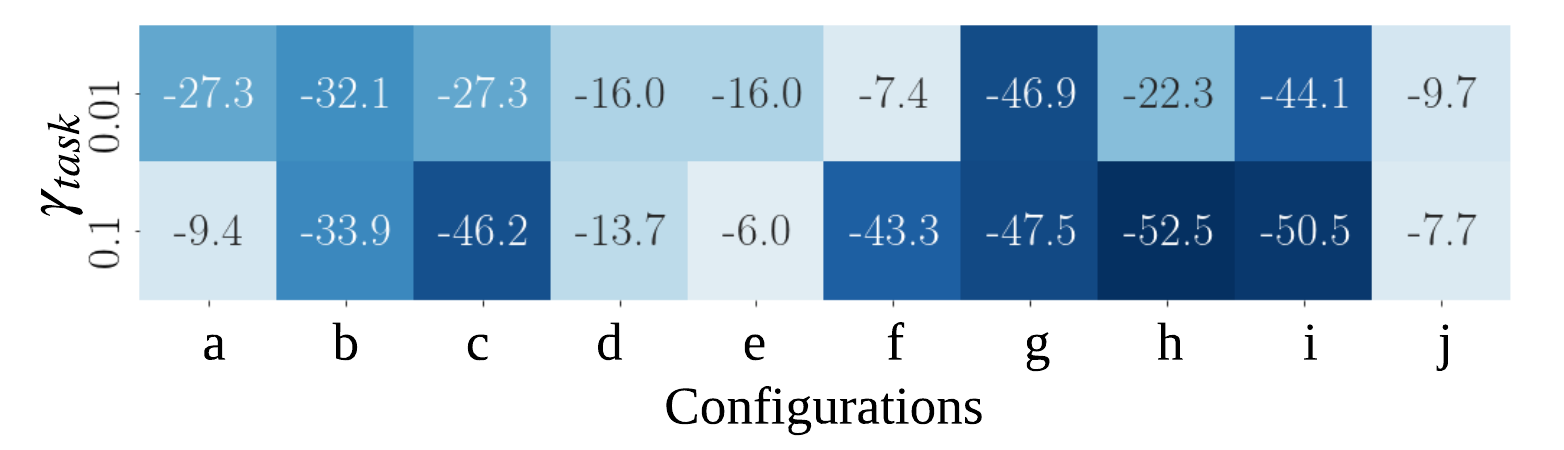
\includegraphics[width=.6\textwidth]{adkl/ablation/gamma-task}
  \caption{Relative improvement of the MSE depending on the $\gamma_\mathrm{task}$ parameter}
  \label{fig:app-mine}
\end{figure}


\subsection{Pseudo representation}
\label{app:ablation-pseudo}

\Tab{app-ablation-pseudo} presents the hyper-parameter combinations used in the experiments to assess the impact of the trade-off parameter $\gamma_\mathrm{pseudo}$, which governs the penalty applied to the divergence between the distribution of learned pseudo-representations and the distribution of actual representations. We also repeat \fig{gamma-pseudo} for better readability.

\begin{table}[ht]
    \caption{Effect of the pseudo-examples regularisation (parameter $\gamma_\mathrm{pseudo}$)\\on the MSE performance}
    \centering
    \begin{tabular}{@{}lllllrrr@{}}
        \toprule
                   &    &                  &      & $\gamma_\mathrm{pseudo}$ &    0.00 &    0.01 &    0.10 \\
        algorithm & K & architecture & $\gamma_\mathrm{task}$ & Conf. &         &         &         \\
        \midrule
        ADKL-GP & 10 & deepset & 0.10 & a  &  0.6079 &  \textbf{0.4352} &  0.5244 \\
                   & 20 & deepset & 0.01 & b  &  0.0873 &  \textbf{0.0761} &  0.0882 \\
        ADKL-KRR & 20 & deepset & 0.00 & c  &  0.0526 &  \textbf{0.0375} &  0.0380 \\
        ADKL-GP & 5  & attention & 0.10 & d  &  2.2801 &  \textbf{2.2112} &  2.2994 \\
        ADKL-KRR & 20 & deepset & 0.01 & e  &  0.0535 &  \textbf{0.0325} &  \textbf{0.0325} \\
        ADKL-GP & 5  & deepset & 0.01 & f  &  2.9466 &  2.7663 &  \textbf{2.7121} \\
                   & 20 & attention & 0.10 & g  &  0.1147 &  0.1144 &  \textbf{0.0870} \\
                   &    & deepset & 0.00 & h  &  0.1201 &  0.0958 &  \textbf{0.0940} \\
                   & 5  & attention & 0.01 & i  &  3.1136 &  \textbf{2.1511} &  2.2511 \\
                   &    &                  & 0.00 & j &  2.8528 &  2.5611 &  \textbf{2.4920} \\
        \bottomrule
    \end{tabular}
    \label{tab:app-ablation-pseudo}
\end{table}

\begin{figure}[ht]
    \centering
    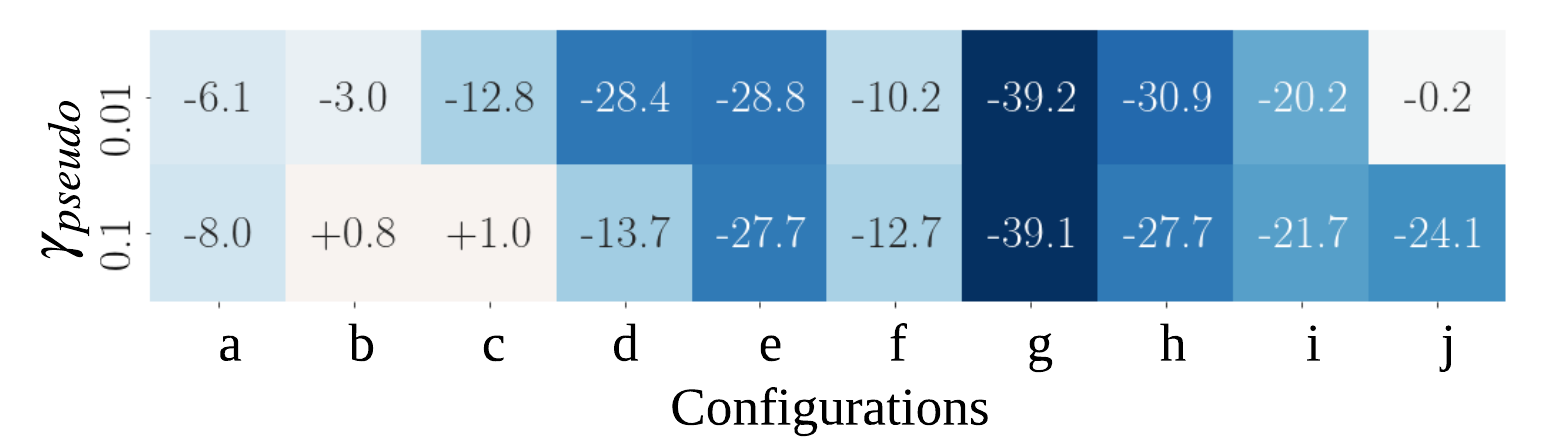
\includegraphics[width=.6\textwidth]{adkl/ablation/heatmap_pseudo}
    \caption{Relative improvement of the MSE depending on the $\gamma_\mathrm{task}$ parameter}
    \label{fig:app-pseudo}
\end{figure}

% Overall, the effect of the regularisation is beneficial, even though we witness a few pathological cases.

\subsection{Joint impact of the task and pseudo-representation regularisations}
\label{app:ablation-task-pseudo}

Since both $\gamma_\mathrm{task}$ and $\gamma_\mathrm{pseudo}$ have a high impact on the training and the generalization performance, we need to assess the relationship between the two.
\Fig{app-pseudo-task} shows for different values of $|\Dsupport|$ the relative improvement of the test MSE compared to the case where no regularisation is done.
Overall, higher is better in both dimensions, although there seems to be a sweet spot on the grid for each value of $|\Dsupport|$ and therefore we can only advise the user to cross-validate on those hyper-parameters.


\begin{figure}[ht]
    \centering
    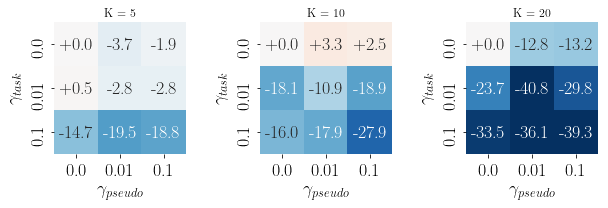
\includegraphics[width=.7\textwidth]{adkl/ablation/heatmap_task_pseudo_metakrr_mk2.png}
    \caption{Average relative improvement of the MSE\\and joint impact of $\gamma_\mathrm{task}$ and $\gamma_\mathrm{pseudo}$.}
    \label{fig:app-pseudo-task}
\end{figure}


\clearpage
\section{Prediction curves on the Sinusoids collection}
\label{app:predictions}

\Fig{app-predictions} presents a visualization of the results obtained by each model on three tasks taken randomly from the meta-test set in the \texttt{Sinusoids} collection.

\begin{figure}[ht]
    \centering
    \begin{subfigure}{.3\textwidth}
        \centering
        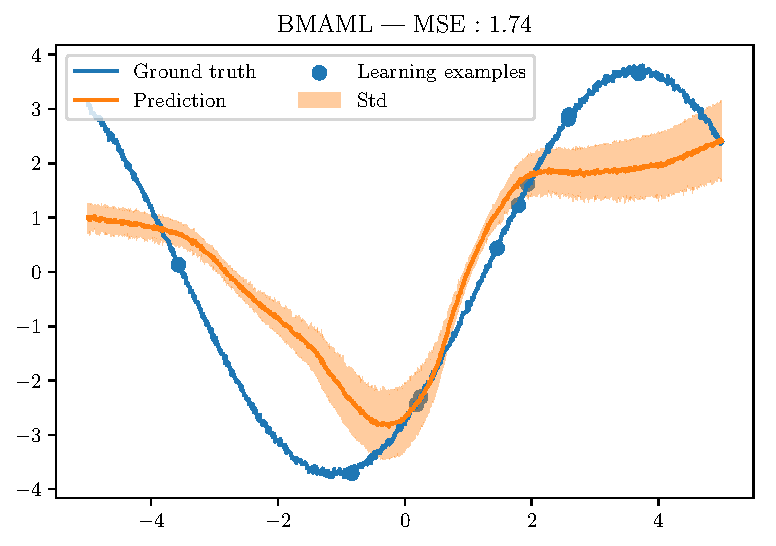
\includegraphics[width=\textwidth]{adkl/predictions/BMAML-18}
    \end{subfigure}
    \hfill
    \begin{subfigure}{.3\textwidth}
        \centering
        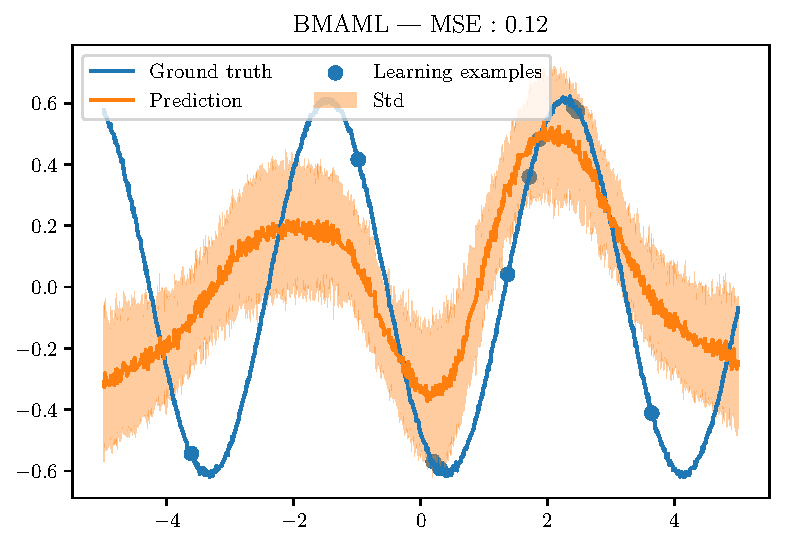
\includegraphics[width=\textwidth]{adkl/predictions/BMAML-15}
    \end{subfigure}
    \hfill
    \begin{subfigure}{.3\textwidth}
        \centering
        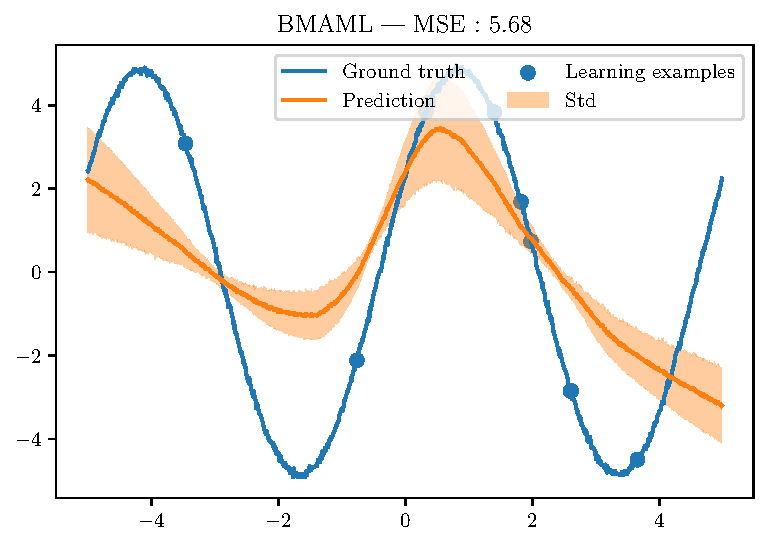
\includegraphics[width=\textwidth]{adkl/predictions/BMAML-4}
    \end{subfigure}
    \\
    \begin{subfigure}{.3\textwidth}
        \centering
        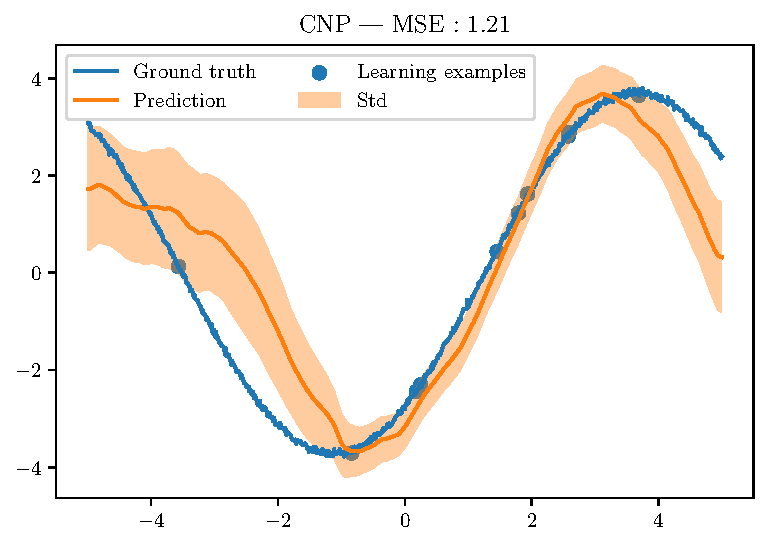
\includegraphics[width=\textwidth]{adkl/predictions/CNP-18}
    \end{subfigure}
    \hfill
    \begin{subfigure}{.3\textwidth}
        \centering
        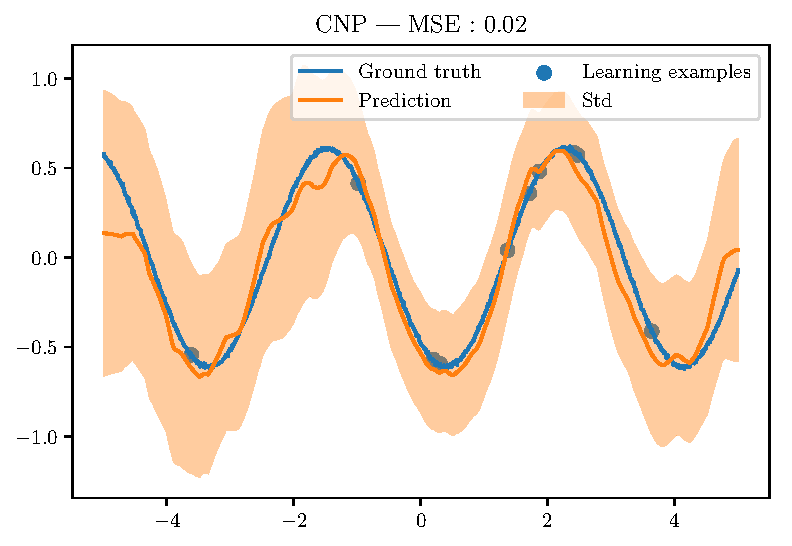
\includegraphics[width=\textwidth]{adkl/predictions/CNP-15}
    \end{subfigure}
    \hfill
    \begin{subfigure}{.3\textwidth}
        \centering
        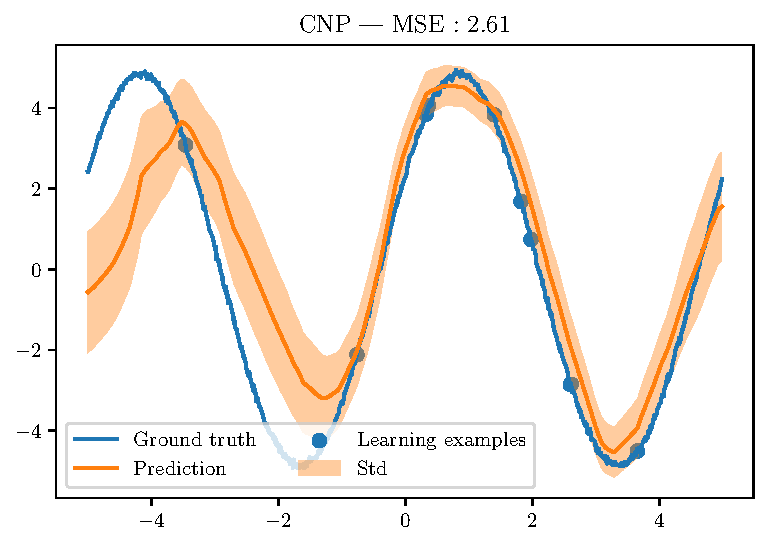
\includegraphics[width=\textwidth]{adkl/predictions/CNP-4}
    \end{subfigure}
    \\
    \begin{subfigure}{.3\textwidth}
        \centering
        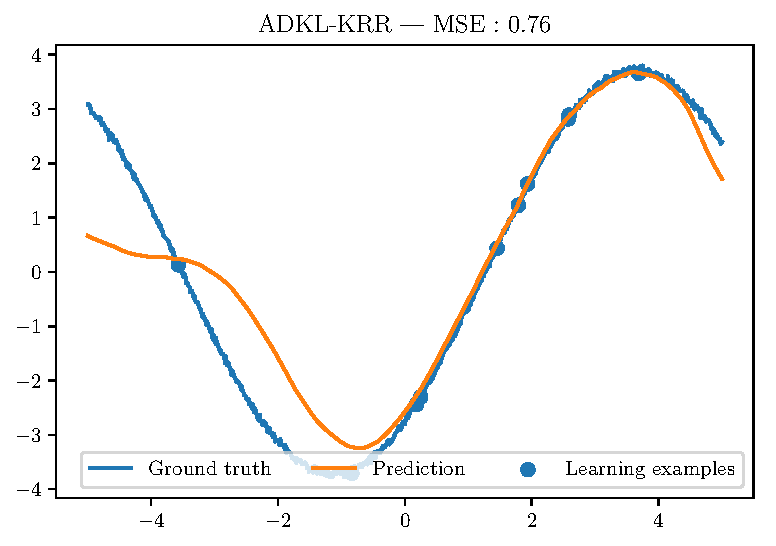
\includegraphics[width=\textwidth]{adkl/predictions/ADKL-KRR-18}
    \end{subfigure}
    \hfill
    \begin{subfigure}{.3\textwidth}
        \centering
        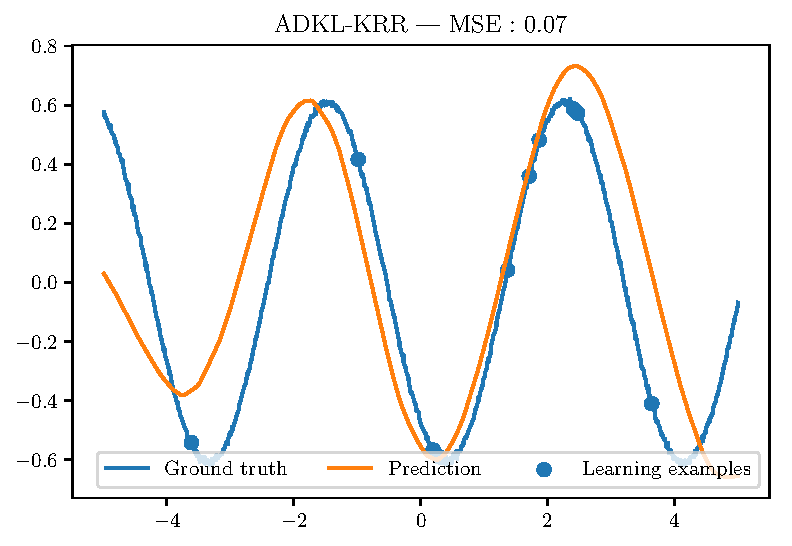
\includegraphics[width=\textwidth]{adkl/predictions/ADKL-KRR-15}
    \end{subfigure}
    \hfill
    \begin{subfigure}{.3\textwidth}
        \centering
        \includegraphics[width=\textwidth]{adkl/predictions/ADKL-KRR-4}
    \end{subfigure}
    \\
    \begin{subfigure}{.3\textwidth}
        \centering
        \includegraphics[width=\textwidth]{adkl/predictions/MAML-18}
    \end{subfigure}
    \hfill
    \begin{subfigure}{.3\textwidth}
        \centering
        \includegraphics[width=\textwidth]{adkl/predictions/MAML-15}
    \end{subfigure}
    \hfill
    \begin{subfigure}{.3\textwidth}
        \centering
        \includegraphics[width=\textwidth]{adkl/predictions/MAML-4}
    \end{subfigure}
    \\
    \begin{subfigure}{.3\textwidth}
        \centering
        \includegraphics[width=\textwidth]{adkl/predictions/ADKL-GP-18}
    \end{subfigure}
    \hfill
    \begin{subfigure}{.3\textwidth}
        \centering
        \includegraphics[width=\textwidth]{adkl/predictions/ADKL-GP-15}
    \end{subfigure}
    \hfill
    \begin{subfigure}{.3\textwidth}
        \centering
        \includegraphics[width=\textwidth]{adkl/predictions/ADKL-GP-4}
    \end{subfigure}
    % \\
    % \begin{subfigure}{.3\textwidth}
    %     \centering
    %     \includegraphics[width=\textwidth]{adkl/predictions/R2-D2-18}
    % \end{subfigure}
    % \hfill
    % \begin{subfigure}{.3\textwidth}
    %     \centering
    %     \includegraphics[width=\textwidth]{adkl/predictions/R2-D2-15}
    % \end{subfigure}
    % \hfill
    % \begin{subfigure}{.3\textwidth}
    %     \centering
    %     \includegraphics[width=\textwidth]{adkl/predictions/R2-D2-4}
    % \end{subfigure}
    \caption{Meta-test time predictions on the \texttt{Sinusoids} collection}
    \label{fig:app-predictions}
\end{figure}


\end{document}
